%%%%%%%%%%%%%%%%%%%%%%% file template.tex %%%%%%%%%%%%%%%%%%%%%%%%%
%
% This is a template file for the global option of the SVJour class
%
% Copy it to a new file with a new name and use it as the basis
% for your article
%
%%%%%%%%%%%%%%%%%%%%%%%% Springer-Verlag %%%%%%%%%%%%%%%%%%%%%%%%%%
%
%% First comes an example EPS file -- just ignore it and
%% proceed on the \documentclass line
%\begin{filecontents*}{example.eps}
%%!PS-Adobe-3.0 EPSF-3.0
%%%BoundingBox: 19 19 221 221
%%%CreationDate: Mon Sep 29 1997
%%%Creator: programmed by hand (JK)
%%%EndComments
%gsave
%newpath
%  20 20 moveto
%  20 220 lineto
%  220 220 lineto
%  220 20 lineto
%closepath
%2 setlinewidth
%gsave
%  .4 setgray fill
%grestore
%stroke
%grestore
%\end{filecontents*}
%
% Choose either the first of the next two \documentclass lines for one
% column journals or the second for two column journals.
%\documentclass[global,referee]{svjour}
\documentclass[global,twocolumn]{svjour}
%\documentclass[global,twocolumn,referee]{svjour}
% Remove option referee for final version
%
% Remove any % below to load the required packages
%\usepackage{latexsym}

\usepackage[table,xcdraw]{xcolor}
\usepackage{amsmath}
\usepackage[utf8]{inputenc}
\usepackage[T1]{fontenc}
\usepackage{lmodern}
\usepackage[english]{babel}
\usepackage{microtype} % optional, for aesthetics
\usepackage{tabularx} % nice to have
\usepackage{booktabs} % necessary for style
\usepackage{graphicx}
\graphicspath{{./figures/}}
\usepackage{listings}
\usepackage{cite}
\usepackage{multirow}
\usepackage{hhline}
\usepackage{caption}
\usepackage{makecell}
\usepackage{ragged2e}
\usepackage{parskip}
\usepackage{wrapfig}
\usepackage{array}
\usepackage{float}
\usepackage{lipsum}
\usepackage{subcaption}
\usepackage[linesnumbered,ruled]{algorithm2e}
\usepackage{courier}
\usepackage{hyperref}
\hypersetup{colorlinks=true,allcolors=blue}
\usepackage{listings}
\usepackage{float}
\lstset{
    basicstyle=\ttfamily,
    frame=none, 
    breaklines=true,
    numbers=left,
    xleftmargin=2.5em,
    framexleftmargin=0em,
    emphstyle=\textbf,
    float=t
}
\lstdefinestyle{ocl}{
    emph={
        context, inv
    }
}
\lstdefinestyle{cbp}{
    basicstyle=\ttfamily\scriptsize,
    emph={
        session, create, type,
        set, to, add, hire
    }
}
\lstdefinestyle{xmi}{
    basicstyle=\ttfamily\scriptsize,
    emph={
        Node, children
    }
}
\lstdefinestyle{xml}{
    basicstyle=\ttfamily\scriptsize,
    emph={
        register, create, add, to, resource, at,
        from, eattribute, remove, ereference,
        set, unset, session, Roy, Jen,
        Moss, Richmond
    }
}
\lstdefinestyle{java}{
    basicstyle=\ttfamily\scriptsize,
    emph={
        case, $unset$,
        instanceof, else, if, void,
        new, UnsetEAttributeEvent,
        UnsetEReferenceEvent,
        @override, public, class, extends
    }
}
\lstdefinestyle{eol}{
    basicstyle=\ttfamily\scriptsize,
    emph={
        var, new, for, in, create, set, with, type, at,
        unset, to, add, remove, delete, register, move,
        from, position, from, move-within, session, comp, composite, \.
    }
}

% etc
%
% Insert the name of "your" journal with the command below:
\journalname{myjournal}
%
\begin{document}
    
\renewcommand{\thelstlisting}{\arabic{lstlisting}}
\renewcommand{\labelitemi}{$\bullet$}
\newcommand{\AndA}{\textnormal{\textbf{and }}}
\newcommand{\Is}{\textnormal{\textbf{is }}}
\newcommand{\Not}{\textnormal{\textbf{not }}}
\newcommand{\In}{\textnormal{\textbf{in }}}
\newcommand{\Or}{\textnormal{\textbf{or }}}
\newcommand{\eqnum}{\refstepcounter{equation}\textup{\tagform@{\theequation}}}

%
\title{Conflict Detection using Change-based Persistence}
%\subtitle{Do you have a subtitle?\\ If so, write it here}
\author{Alfa Yohannis\inst{1,3} \and Horacio Hoyos Rodriguez\inst{1} \and Fiona Polack\inst{2} \and Dimitris Kolovos\inst{1}% etc
% \thanks is optional - remove next line if not needed
%\thanks{\emph{Present address:} Insert the address here if needed}%
}                     % Do not remove
%
\offprints{}          % Insert a name or remove this line
%
\institute{Department of Computer Science, University of York, United Kingdom  
    \and School of Computing and Maths, Keele University, United Kingdom
    \and Department of Computer Science, Kalbis Institute, Indonesia}
%
\date{Received: 1 July 2019 / Revised version: 1 August 2019}
% The correct dates will be entered by the editor
%
\maketitle
%
\begin{abstract}
Comparison -- difference identification and conflict detection -- of large models can be time-consuming since every element has to be visited, matched, and compared with its respective element in other models. This can result in bottlenecks in collaborative modelling environments, where identifying differences between two versions of a model is desirable. Reducing the comparison process to only the elements that have been modified since a previous known state (e.g. previous version) could significantly reduce the time required for large model comparison. This paper presents how change-based persistence can be used to localise the comparison of models so that only elements affected by recent changes are compared and to substantially reduce comparison and differencing time (up to 90\% in some experiments) compared to state-based model comparison. 
\end{abstract}
%

\section{Introduction}
\label{sec:introduction}

\vspace{-5pt}

In modelling and model management, it is common to find that many versions or variants of a model exist. These versions are commonly persisted as snapshots of the model at a given point in time, in a state-based format such as XMI. Model comparison activities can be applied to the different versions of a model to highlight their differences: changes in properties values, new elements, etc. However, comparing versions of large file-based\footnote{Persisting models in databases involves its own challenges which have been discussed extensively in the literature. For the rest of the paper, we are only concerned with file-based models and we return to database-backed model representations in Section \ref{sec:related_work}.} models in a state-based format can be computationally expensive since both versions of the model need to be loaded in memory in their entirety before their elements can be matched and diffed. %This pairwise comparison can slow down the modelling tasks in a collaborative modelling setting. 

In our previous work \cite{DBLP:conf/models/YohannisKP17,yohannis2018towards,DBLP:conf/models/YohannisRPK18}, we proposed change-based persistence (CBP) as an alternative approach to state-based persistence of EMF models \cite{steinberg2008emf}. Instead of persisting models as XMI snapshots, in the proposed approach models are persisted as a complete history of changes. We demonstrated the substantial performance benefits of CBP in terms of saving changes to large models \cite{DBLP:conf/models/YohannisKP17} as well as a method for reducing model loading time compared to naively replaying all recorded change events \cite{DBLP:conf/models/YohannisRPK18} to reconstruct the state of a change-based model. 
In this paper, we demonstrate how a change-based representation also enables much more efficient and performant model comparison between versions of the same model. Our experiments, presented in Section \ref{sec:evaluation}, demonstrate savings of the order of 90\% for (relatively) small changes made to large models.

This paper is structured as follows. Section \ref{sec:change-based_persistence} provides an overview of our previous work on change-based model persistence. Section \ref{sec:model_comparison} discusses state-based model comparison. Section \ref{sec:change_based_approach_for_comparing_models} presents our change-based approach to speed up model comparison and its implementation. Section \ref{sec:evaluation} 
%\dk{Consolidate sections 5 and 6?} 
reports on the results of evaluation experiments used to evaluate the proposed approach. Section \ref{sec:related_work} provides an overview of related work, and Section \ref{sec:conclusion_and_future_work} concludes with a discussion on directions for future work.

\vspace{-10pt}
\section{Change-based Persistence}
\label{sec:change-based_persistence}

\vspace{-5pt}
CBP is an alternative approach to state-based persistence (SBP) of models. Instead of persisting snapshots of the state of a model -- which is the default behaviour of frameworks such as EMF -- CBP persists the entire history of change events of a model \cite{yohannis2018towards}. For example, in SBP approach, when we save the UML class diagram in Fig. \ref{fig:origin} in standard XMI format, we only record the last state of the model, as shown in List. \ref{lst:originxmi}. In contrast, when we develop the same model in CBP approach, all the change events generated from modifying the model are captured and persisted in the model file as shown in List. \ref{lst:origincbp}\footnote{In our implementation, the change-based format is XML-based.}. 
%The file consists of events generated by changes \dk{Isn't event === change? Do we need to use both terms? If so, we should explain their difference}. 
Each change event contains information about the type of the operation applied as well the as values, elements, or features involved. Replaying the change events in List. \ref{lst:origincbp} produces the same eventual model as in Fig. \ref{fig:origin}.

\vspace{-15pt}
\begin{lstlisting}[style=eol,caption={The simplified XMI of the model in Fig. \ref{fig:origin}.},label=lst:originxmi]
<uml:Class id="x" name="Math">
<operation id="a" name="abs"/>
<operation id="b" name="mean"/>
<operation id="c" name="pow"/>
</uml:Class>
\end{lstlisting}

\vspace{-10pt}
\begin{figure}[H]
    \centering    
    \hfill
    \begin{subfigure}[t]{0.2\linewidth}
        \centering
        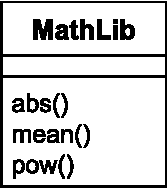
\includegraphics[width=\linewidth]{OriginalClassDiagram}
        \caption{origin}
        \label{fig:origin}
    \end{subfigure}
    \hfill
    \begin{subfigure}[t]{0.2\linewidth}
        \centering
        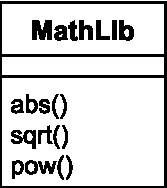
\includegraphics[width=\linewidth]{LeftClassDiagram}
        \caption{left}
        \label{fig:left}
    \end{subfigure}
    \hfill
    \begin{subfigure}[t]{0.2\linewidth}
        \centering
        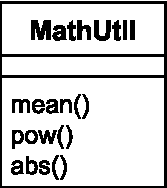
\includegraphics[width=\linewidth]{RightClassDiagram}
        \caption{right}
        \label{fig:right}
    \end{subfigure}
    \hfill
    \label{fig:versions}
    \caption{Different versions of a model.}
\end{figure}

\begin{lstlisting}[style=eol,caption={The pseudo-formatted CBP of the model in Fig. \ref{fig:origin}.},label=lst:origincbp]
create x type Class
set x.name to "Math" 
create a type Operation
set a.name to "abs" 
create b type Operation
set b.name to "mean" 
create c type Operation
set c.name to "pow" 
add a to x.operations at 0
add b to x.operations at 1
add c to x.operations at 2
\end{lstlisting}

\vspace{-5pt}
\section{State-based Model Differencing}
\label{sec:model_differencing}

\vspace{-5pt}
In a collaborative modelling setting, a model can have different versions.
%\dk{Mutliple versions can exist even if a model is developed by a single developer}.
Consider the case where an initial version of a model exists in a Version Control System (VCS) server (Fig. \ref{fig:vcs}).
Two modellers, Bob and Alice, check out the original model (steps 1 and 2) to their local machines and modify it (steps 3 and 4).
Alice then commits her work (original + Alice's changes) to the VCS.
Since there is no newer commit on the VCS, the commit process is straightforward (step 5).
Bob then decides to also commit his work (original + Bob's changes) to the VCS.
However, he needs to merge his work with the current updated version at the VCS since his last checkout.
His machine downloads the latest version from the server (step 6), i.e. Alice's version.
To merge his and Alice's changes, Bob needs to perform model comparison to check their differences, resolve possible conflicts between the models, and then merge them (step 7).
After that, he can push it back to the VCS server.

\begin{figure}[ht]
    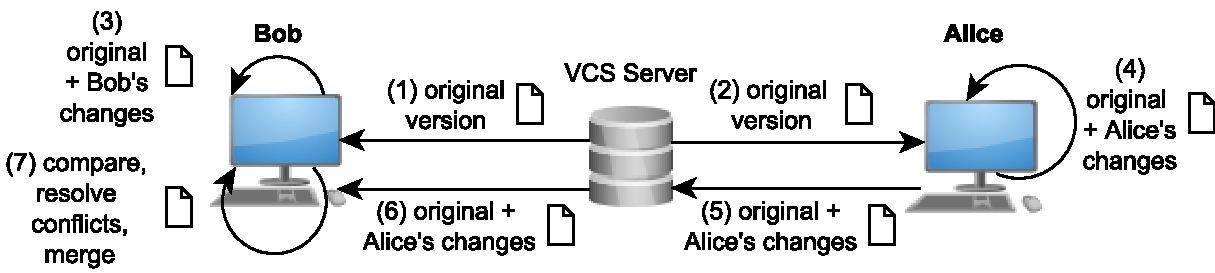
\includegraphics[width=\linewidth]{VCS}
    \caption{A usecase of CBP in a collaborative modelling.}
    \label{fig:vcs}
\end{figure}


In a SBP setting, Bob produces the model in Fig. \ref{fig:left} (the left model), and Alice the model in Fig. \ref{fig:right} (the right model) producing XMI files as shown in List. \ref{lst:leftxmi} and List. \ref{lst:rightxmi} respectively.
Before Bob can merge, he must compare the right model with the left model.
In state-based comparison, comparing models commonly consists of two steps: \emph{matching} and \emph{diffing}.
The matching process establishes matches between the elements of both models, to determine the elements in the left model that correspond to elements in the right model.
Generally, the matching process iterates through all the elements of the models being compared and matches them by their identifiers or through a similarity mechanism  \cite{DBLP:conf/sfm/BroschKLSWW12,emfcompare2018developer}.
%Note that for new and deleted elements the result of the match can be that there is no match.

The diffing process identifies differences between the matched elements \cite{DBLP:conf/sfm/BroschKLSWW12,emfcompare2018developer}.
Differences between the matched elements and all their features is usually done using a Longest Common Subsequence (LCS) algorithm, e.g. \cite{DBLP:journals/algorithmica/Meyers86}.

\vspace{-10pt}
\begin{lstlisting}[style=eol,caption={The simplified XMI of the left model in Fig. \ref{fig:left}.},label=lst:leftxmi]
<uml:Class id="x" name="MathLib">
<operation id="a" name="abs/>
<operation id="d" name="sqrt"/>
<operation id="c" name="pow"/>
</uml:Class>
\end{lstlisting}

\begin{lstlisting}[style=eol,caption={The simplified XMI of the right model in Fig. \ref{fig:right}.},label=lst:rightxmi]
<uml:Class id="x" name="MathUtil">
<operation id="b" name="mean"/>
<operation id="c" name="pow"/>
<operation id="a" name="abs"/>
</uml:Class>
\end{lstlisting}

In our example, the matching process in state-based comparison -- as performed by EMF Compare \cite{emfcompare2018developer} -- iterates through all the elements of both models and matches them using their identifiers. The matching process yields 3 matches: $m_1$ = (\textsf{x}, \textsf{x}), $m_2$ = (\textsf{a}, \textsf{a}), and $m_3$ = (\textsf{c}, \textsf{c}), and 2 unmatched elements, $um_1$ = (\textsf{d}, -) and $um_2$ = (-, \textsf{b}). The diffing process then iterates through all the matches and unmatched elements and uses an LCS algorithm to identify their differences. In the first match, it identifies that the elements \textsf{x} are different in their \textsf{name} and \textsf{operations} features. 

The left \textsf{x}'s \textsf{name} is ``MathLib'' while the other \textsf{x}'s \textsf{name} is ``MathUtil'' (diff $ds_1$). The \textsf{operations} features are different in their contents -- the left \textsf{operations} feature does not contain element \textsf{b} (diff $ds_2$), the left \textsf{operations} feature contains element \textsf{d} 
that does not exist in the right \textsf{operations} (diff $ds_3$), and the indexes of element \textsf{c} are different in both features (diff $ds_4$).

Differences are commonly expressed as a list of changes that must be applied to a target model so that it is made equal to a reference model.
%\dk{We should probably consider different terminology here as the terms ``source'' and ``reference'' are very similar}.
This paper treats the left model as a reference model and the right model as the target model.
This means that differences are expressed as changes applied to the right model so that it equals the left model.
To express differences, we use the following terms: \textsf{LeftContainer}, \textsf{RightContainer}, \textsf{LeftFeature}, \textsf{RightFeature} \textsf{LeftIndex}, \textsf{RightIndex}, \textsf{LeftValue}, \textsf{RightValue}, and \textsf{Kind}. The \textsf{*Container}, \textsf{*Feature}, and \textsf{*Value} are the target element, feature, and value involved in a difference (\textsf{*} symbol can be replaced with \textsf{Left} and \textsf{Right}). \textsf{*Index} is the index of a value in a feature. \textsf{Kind} is the type of difference. It can be one of these types: \textsf{CHANGE}, \textsf{ADD}, \textsf{DELETE}, and \textsf{MOVE}. \textsf{CHANGE} means a pair of single-valued features 
%features -- single-valued attributes or non-containment references \dk{Why is containment important?} -- 
have different values. \textsf{ADD} indicates that a value does not exist in the right model thus it requires the addition of the value. \textsf{DELETE} is the opposite
%\dk{``opposite''?} 
of \textsf{ADD}. \textsf{MOVE} indicates that matched elements differ in terms of their containers, containing features, or indexes.
A Container is an element that contains a value. A containing feature is a feature owned by a container in which a value is contained. An index is the position of a value in a containing feature.

Based on these definitions, we can express the result of the diffing process as a tuple:
\begin{equation} \label{eq:diff_definition}
\begin{split}
ds_{n} = &[LeftContainer_n, RightContainer_n,\\
&LeftFeature_n, RightFeature_n,\\
&LeftIndex_n, RightIndex_n,\\
&LeftValue_n, RightValue_n, Kind_n]
\end{split}
\end{equation}

Thus, $ds_{1}$ =  [\textsf{x}, \textsf{x}, \textsf{name}, \textsf{name}, 0, 0, ``MathLib'', ``Mathutil'', \textsf{CHANGE}], $ds_{2}$ = [\textsf{x}, \textsf{x}, \textsf{operations}, \textsf{operations}, null, 0, null, \textsf{b}, \textsf{DELETE}], $ds_{3}$ = [\textsf{x}, \textsf{x}, \textsf{operations}, \textsf{operations}, 1, null, \textsf{d}, null, \textsf{ADD}], and $ds_{4}$ = [\textsf{x}, \textsf{x}, \textsf{operations}, \textsf{operations}, 2, 1, \textsf{c}, \textsf{c}, \textsf{MOVE}]. We can use these information to represent the differences visually as depicted in Fig. \ref{fig:xmi_comparison}. Applying these differences as changes to the right model will transform it into the left model.  

\begin{figure}
    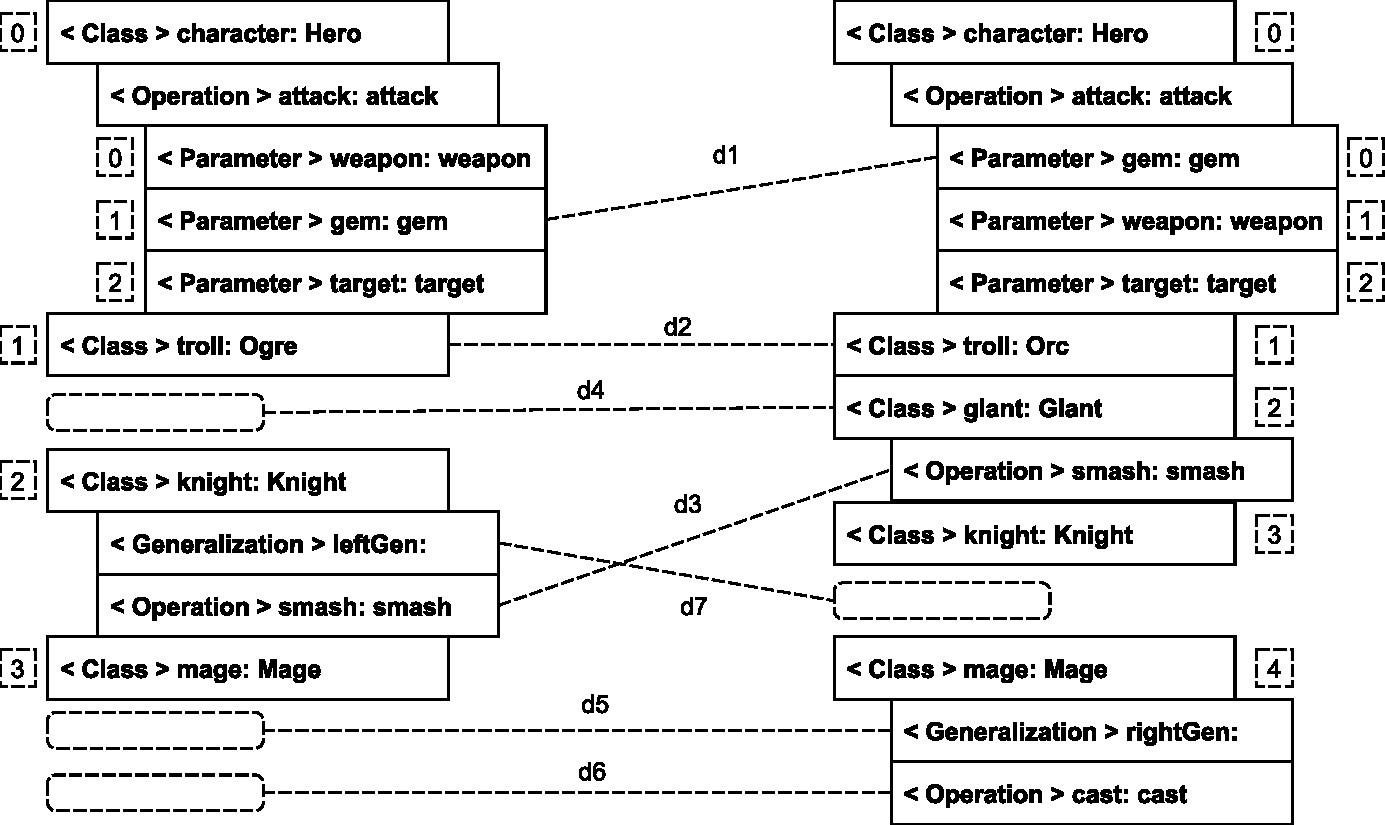
\includegraphics[width=\linewidth]{XmiComparison}
    \caption{A model comparison of the left and right models in Listings \ref{lst:leftxmi} and \ref{lst:rightxmi}.}
    \label{fig:xmi_comparison}
\end{figure}

\begin{figure*}[t]
    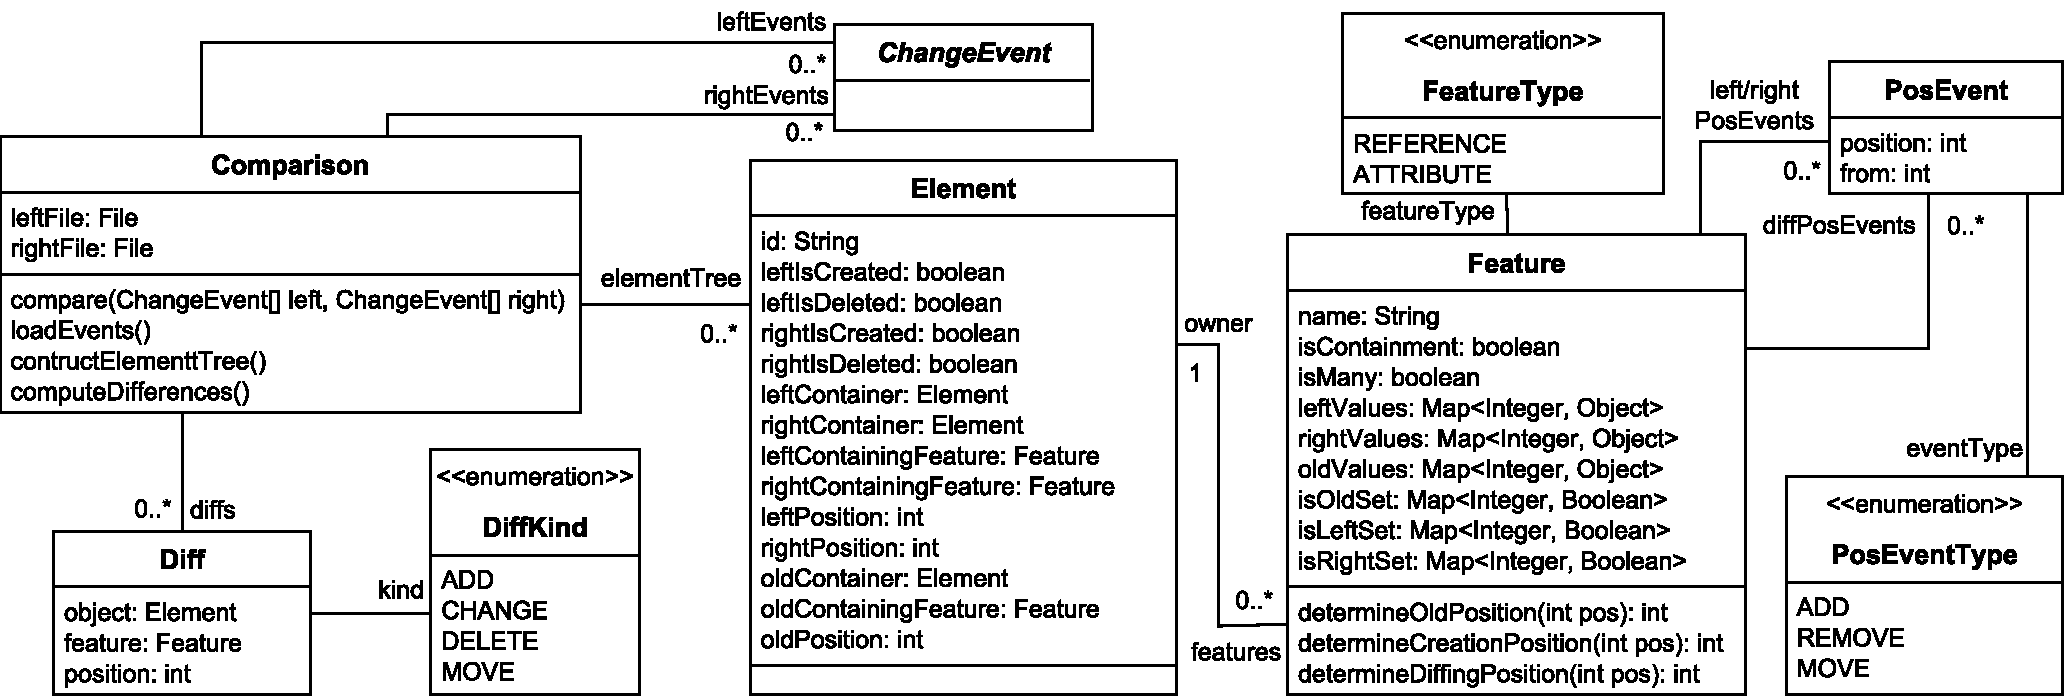
\includegraphics[width=\linewidth]{TreeClassDiagram}
    \caption{A class diagram showing the core components of the change-based approach to speed up model comparison.}
    \label{fig:approach_class_diagram}
\end{figure*}

\section{Change-based Approach for Comparing Models}
\label{sec:change_based_approach_for_comparing_models}

Now lets consider the same example in a CBP setting.
The changes made by Bob and Alice are appended to the their local original CBP producing two different CBP representations as displayed in Listings \ref{lst:leftcbp} and \ref{lst:rightcbp}\footnote{Both CBPs only present the changes after the last line of the original version (start from line 12).} -- capturing different courses of modification made by the two modellers.
Then the example is the same with Alice committing her changes and Bob wanting to merge Alice's work with his. 

\vspace{-10pt}
\begin{lstlisting}[firstnumber=12,style=eol,caption={The appended changes made by Bob to produce the model in Fig. \ref{fig:left} (left version).},label=lst:leftcbp]
set x.name from "Math" to "MathLib"
create d type Operation
set d.name to "sqrt"
add d to x.operations at 1
remove b in x.operations at 2
delete b
\end{lstlisting}

\vspace{-15pt}
\begin{lstlisting}[firstnumber=12,style=eol,caption={The appended changes made by Alice to produce the model in Fig. \ref{fig:right} (right version).},label=lst:rightcbp]
move a in x.operations from 0 to 2
set x.name from "Math" to "MathUtil"
\end{lstlisting}

%Since both modellers work using CBP, we can exploit the representation to improve the previous model comparison.
%For example, we do not need to visit, match, and differentiate both \textsf{c} elements in the running example as they are not affected by the recent changes in both CBPs; only the affected features by the recent changes to be compared -- not all features. 
In CBP, comparison has three phases: event loading, element tree construction, and diff computation.
Further, comparison is not performed over all the elements of the model; instead, we only need to compare the last set of changes from the source and reference model.
The last set of changes can be easily identified by finding their last common change.
A simplified class diagram of our approach's implementation\footnote{The source can be found at \url{https://github.com/epsilonlabs/emf-cbp}.} is depicted in Fig. \ref{fig:approach_class_diagram}. 
Next, we describe the three phases in detail.

\subsection{Event Loading}
\label{sec:event_loading}
In the event loading phase, our implementation loads change events recorded in two CBP files into memory.
The most important aspect of this phase is the partial loading as only lines starting from the position where the two files are different are loaded.
Thus, not the whole model needs to be traversed and loaded.
In this case, lines 1-11 in List. \ref{lst:origincbp} are skipped.

Only lines starting from line 12 in Listings \ref{lst:leftcbp} and \ref{lst:rightcbp} are loaded, yielding two partial -- left and right -- change-event models. 

\subsection{Element Tree}
\label{sec:tree_construction}
An element tree is a representation of the changes of model elements in the source and reference models.
It contains detailed information about elements and their properties.

It contains similar information to that captured in change lists in SBP, but also provides more information about the changes.
For example, the element tree can keep track of a feature's old value and element/value's indexes inside multi-valued properties. 
%The latter reduces false-positives when detecting MOVE changes. 
%These specific features are useful to determine differences in the diff computation phase (Section \ref{sec:diff_computation}).
The element tree only contains the partial states of affected elements of the original, left, and right models as depicted in Figures \ref{fig:left_element_tree_diagram} and \ref{fig:right_element_tree_diagram}.

To better understand the construction of an element tree from change events, we use the following running example using both change events in the Listings \ref{lst:leftcbp} and \ref{lst:rightcbp}. We start from the left change events. 

\begin{figure}
    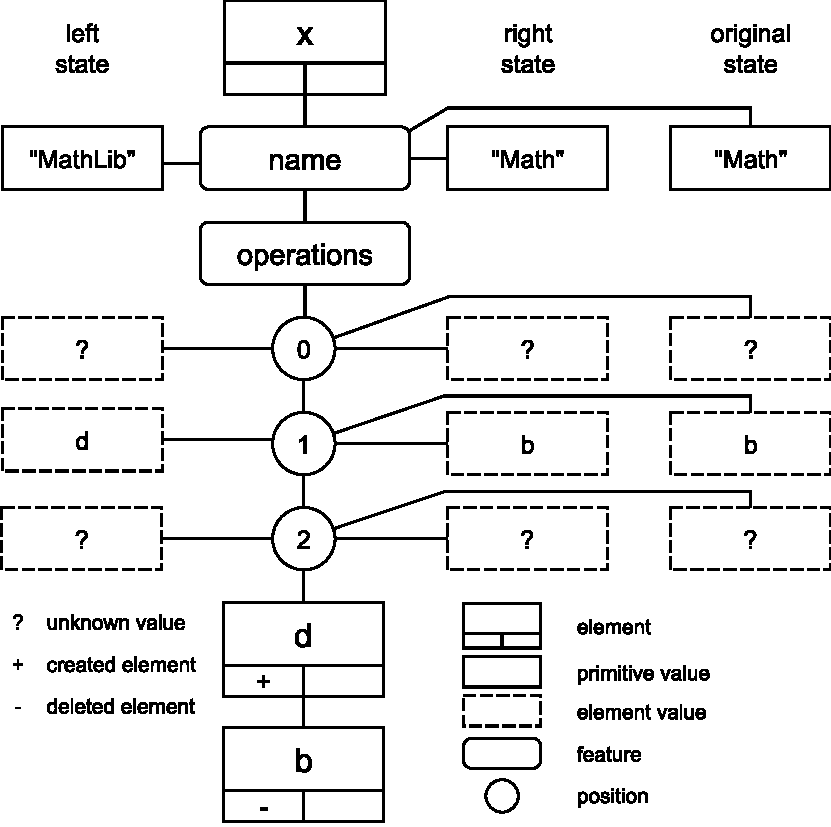
\includegraphics[width=\linewidth]{LeftElementTreeDiagram}
    \caption{The \textsf{elementTree} after processing all left change events.}
    \label{fig:left_element_tree_diagram}
\end{figure}

\begin{figure}
    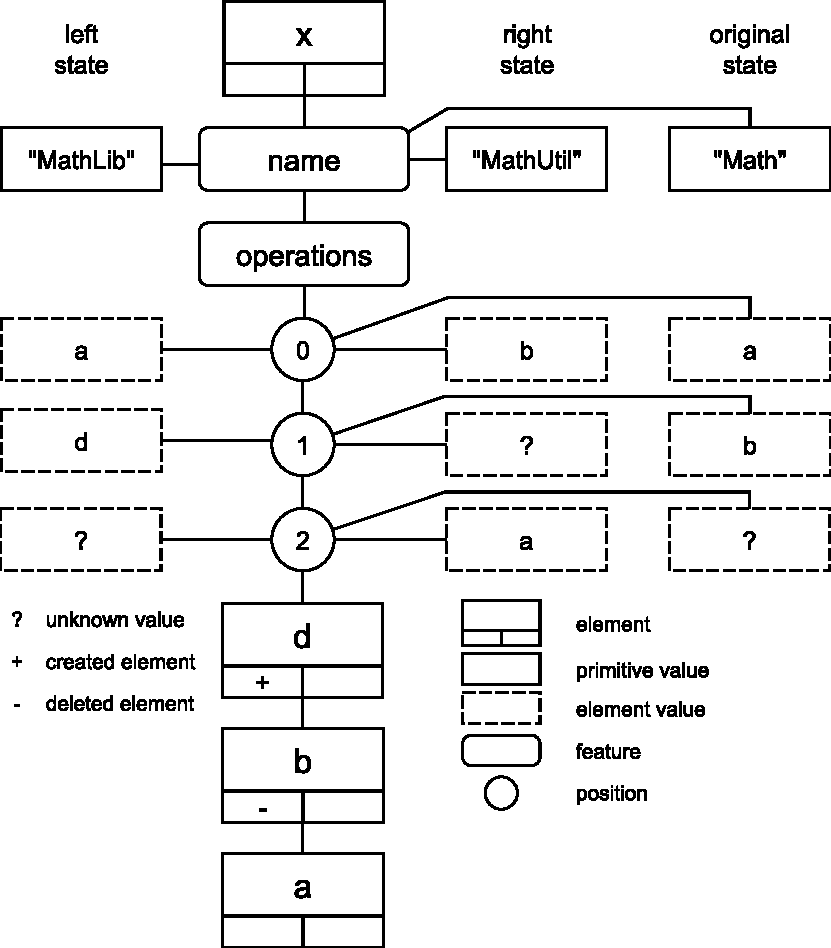
\includegraphics[width=\linewidth]{RightElementTreeDiagram}
    \caption{The \textsf{elementTree} after processing all left and right change events.}
    \label{fig:right_element_tree_diagram}
\end{figure}

\subsubsection{Left Side}\label{sec:left_side}
%In List. \ref{lst:leftcbp}, 

From the first event at line 12, [\texttt{\small \textbf{set} x.name \textbf{from} "Math" \textbf{to} "MathLib"}], we can identify that an element with id \textsf{x} has existed from the original model. 
%\dk{Incomplete sentence?}
It has a feature \textsf{name} with a value ``Math'' in the original model that has been changed to ``MathLib'' in the left model. Since the element \textsf{x} does not already exist in the \textsf{elementTree}, we create its instance of \textsf{Element} and also its feature \textsf{name}. We set the value of the feature \textsf{name} to ``MathLib'' and also set it to ``Math'' in the partial state of the original model -- it has not been set before. As this feature on the right side also has not been set, we set it to ``Math'' as well. 
%Once a feature in the original state has been set, it cannot be overridden -- using the flag \textsf{isOldSet} in class \textsf{Feature} in Fig. \ref{fig:approach_class_diagram}. 

At line 13, in the event [\texttt{\small \textbf{create} d \textbf{type} Operation}], we can identify that an element with id \textsf{d} has been created. We also update the \textsf{elementTree} to include this element and set the element's flag \textsf{leftIsCreated} to \textsf{true}. In the event [\texttt{\small \textbf{set} d.name \textbf{to} "sqrt"}] at line 14, we can identify that element \textsf{d}'s feature \textsf{name} has been set to ``sqrt''. Thus, we update \textsf{d}'s feature \textsf{name} in the \textsf{elementTree}. From the event [\texttt{\small \textbf{add} d \textbf{to} x.operations \textbf{at} 1}] at line 15, we can deduce that element \textsf{d} is added to index 1 in the element \textsf{x}'s feature \textsf{operations}. Thus, we assign \textsf{d} to element \textsf{x}'s feature \textsf{operations} at index 1 in the \textsf{elementTree}. As \textsf{d} is a new element that only exists in the left model, we do not update changes of this element to the original and right models. 

From the event [\texttt{\small \textbf{remove} b \textbf{in} x.operations \textbf{at} 2}] at line 16, we can identify that there is element \textsf{b} in the original model, but it is deleted in the left model. The index of element \textsf{b} in the original model can be calculated back through the previous change events that have been applied to its feature. Since the previous event is adding element \textsf{d} to index 1 and the index of \textsf{b} is at 2 at the time it is removed, we can deduce that before element \textsf{d} is added, the index of element \textsf{b} is at 1 and is shifted to 2 because of the addition of element \textsf{d}.  Therefore, we can conclude that the original index of element \textsf{b} is at 1. Thus, we update the original state of the \textsf{elementTree} by adding element \textsf{b} into the element \textsf{x}'s feature \textsf{operations} at index 1.  

We perform the same procedure to also add element \textsf{b} to the right state of the \textsf{elementTree}. However, since no change event has been applied to the right side of element \textsf{x}'s feature \textsf{operations}, the calculation of element \textsf{b}'s index should return the same value as in the original state (line 13, Alg. \ref{alg:element_tree}), and thus element \textsf{b} has the same index as in the original state. It is important to notice, in this step, the flag \textsf{isRightSet} (class \textsf{Feature}, Fig. \ref{fig:approach_class_diagram}) is not set to \textsf{true} since we want the value to be able to be overridden during processing of the right change events. The last event [\texttt{\small \textbf{delete} b}], removes the element \textsf{b} from the left model. Hence, we set the flag \textsf{leftIsDeleted} of element \textsf{a} to \textsf{true}.

Fig. \ref{fig:left_element_tree_diagram} illustrates the state of the \textsf{elementTree} after all left change events have been processed. As can be seen, the \textsf{elementTree} exhibits the partial states of the original, left, and right models at once. 

\subsubsection{Right Side}\label{sec:right_side}  From the first event at line 12, [\texttt{\small \textbf{move} a \textbf{in} x.operations \textbf{from} 0 \textbf{to} 2}], we can infer that in the right model there is an element with id \textsf{a} positioned at index 2 in the element \textsf{x}'s feature \textsf{operations}. Thus, element \textsf{a} -- an instance of class \textsf{Element} in \ref{fig:approach_class_diagram} -- is added to the \textsf{elementTree} and positioned at index 2 of the element \textsf{x}'s feature \textsf{operations}. Since the event is a \textsf{move} type and the new index is larger than its previous index, elements that are between its previous and new indexes are shifted one place down. As element \textsf{b} has already existed in the same feature (the element was added during the process of the left change events) and its index is between element \textsf{a}'s movement, the index of element \textsf{b} is shifted down from 1 to 0. 

Also since the event's type is \textsf{move} and its previous index is 0 and it is the first event that changes the index of element \textsf{a}, these conditions imply that element \textsf{a} in the original model is positioned at index 0 in the element \textsf{x}'s feature \textsf{operations}. Therefore, we add the element \textsf{a} to element \textsf{x}'s feature \textsf{operations} in the original state of the \textsf{elementTree}. Since the index 0 in the element \textsf{x}'s feature \textsf{operations} has not been set, we also add element \textsf{a} to that index in the right state of the \textsf{elementTree}. From the last event [\texttt{\small \textbf{set} a.name \textbf{from} "Math" \textbf{to} "MathUtil"}] at line 13, we can infer that in the right model, the value of element \textsf{a}'s feature \textsf{name} is ``MathUtil''. Hence, we set the feature \textsf{name} to ``MathUtil'' in the right state. 
We do not apply this operation to the original and left states as they have been set before.
Fig. \ref{fig:right_element_tree_diagram} exhibits the state of the \textsf{elementTree} after both sides' change events have been processed.

\begin{figure}
    \centering
    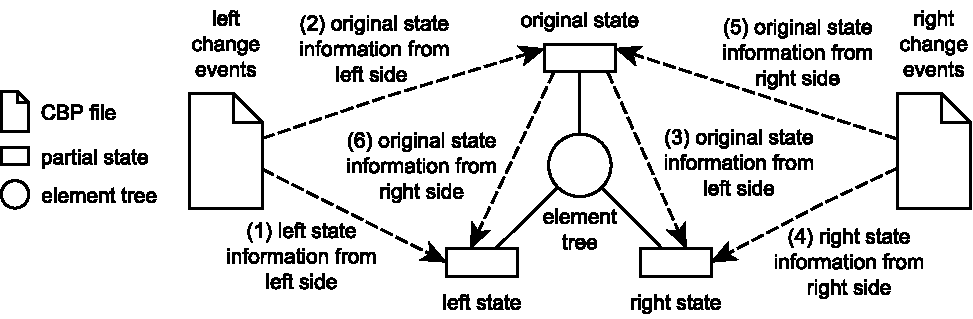
\includegraphics[width=\linewidth]{TreeConstruction}
    \caption{Steps in Element Tree construction.}
    \label{fig:tree_construction}
\end{figure} 

The construction of the \textsf{elementTree} that we have just explained follows the steps shown in Fig. \ref{fig:tree_construction}. First, the partial
%left \dk{Delete ``left''?} 
state $S_{L}$ of the left model in the \textsf{elementTree} is constructed based on the information retrieved from the left change events (step 1). We denote this information as $I_{LL}$. We can also construct the partial 
%original \dk{Delete ``original''?} 
state $S_{O}$ of the original model using the information related to the original state contained in the left change events $I_{OL}$ (step 2). The information $I_{OL}$ allows us to construct the initial partial 
%right \dk{Delete ``right''?} 
state $S_{R}$ of the right model 
%before updated \dk{This doesn't read well} by the right change events 
(step 3). Similarly, using the information from the right change events $I_{RR}$, we update the partial right state $S_{R}$ that has been initialised before using the information $I_{OL}$ (step 4), implying that $I_{OL} \cup I_{RR} \rightarrow S_{R}$. Also, information related to the state of the original model from the right change events $I_{OR}$ is used to update the original state  (step 5). Thus, we have a partial state of the original model constructed using information from both left and right sides, $I_{OL} \cup I_{OR} \rightarrow S_{O}$. Finally, we also use the information $I_{OR}$ to update 
%the left state to have a more representative\dk{Not sure what ``more representative'' means in this context} 
the partial state of the left model (step 6), implying that $I_{LL} \cup I_{OR} \rightarrow S_{L}$.  


\IncMargin{1.5em}
\begin{algorithm}
    \begin{footnotesize}
        \SetKwInOut{Input}{input} 
        \SetKwInOut{Output}{output}
        \Input{a list of ChangeEvent $events$}
        \Input{an enumeration of Side $side$}
        \Input{an instance of ElementTree $elementTree$}
        \Output{an instance of ElementTree $elementTree$}
        \SetKwBlock{Beginn}{beginn}{ende}
        \Begin{
            \ForEach{$event$ in $events$}{
                $targetElement$ $\leftarrow$ getOrCreateNewTargetElement($event$, $elementTree$)\;
                $feature$ $\leftarrow$ getOrCreateNewFeature($event$, $targetElement$)\;
                $value$ $\leftarrow$ getValue($event$)\;
                $previousValue$ $\leftarrow$ getPreviousValue($event$)\;
                $index$ $\leftarrow$ getIndex($event$)\;
                $previousIndex$ $\leftarrow$ getPreviousIndex($event$)\;
                $featureEventList$ $\leftarrow$ getFeatureEventList($feature$, $side$)\;
                
                \BlankLine
                \tcp{put all values to their proper indexes}
                updateTree($targetElement$, $feature$, $value$, $index$, $side$)\;
                $oldIndexes$ $\leftarrow$ calculateOldIndex($featureEventList$, $previousIndex$, $side$)\;
                \If{\Not isCreated($value$, $side$) \AndA \Not isOldValueSet($feature$, $previousValue$, $previousIndex$, $side$)} {
                    setOldValue($feature$, $previousValue$, $oldIndex$, $side$)\;
                    $oppFeaEventList$ $\leftarrow$ getOppFeaEventList($feature$, $side$)\;
                    $oppositeIndex$ $\leftarrow$ calculateOppositeIndex($oppFeaEventList$, $oldIndex$, $side$)\;
                    \If{\Not isDeleted($value$, $side$) \AndA \Not isOppositeSideValueSet($feature$, $value$, $oppositeIndex$, $side$)} {
                        setOppositeSideValue($feature$, $value$, $oppositeIndex$, $side$)\;
                    }
                }   
                
                addEventToFeatureEventList($event$, $featureEventList$)\;
                
            }
            \Return{$elementTree$}\;
        }
    \end{footnotesize}
    \caption{Algorithm to construct an element tree from events.}
    \label{alg:element_tree}
\end{algorithm}
\DecMargin{1.5em}

Alg. \ref{alg:element_tree} describes the steps presented in Fig. \ref{fig:tree_construction} in an generic fashion. It iterates through all a model's change events and uses the information contained in them to construct the relevant partial state. The selection of side, left or right change events, that is executed first depends on the \textsf{Side} enumeration value -- \textsf{left} or \textsf{right} -- passed through the parameter \textsf{side} (the second input parameter). In our implementation, we process the left side first by default. The algorithm also receives an input of the change events \textsf{events} that are to be iterated and the element tree \textsf{elementTree} that has been instantiated before, and then returns the \textsf{elementTree} as output after updating it.

For each \textsf{event} in the \textsf{events}, we collect information needed to build up the \textsf{elementTree}  (lines 3-9), such as \textsf{targetElement}, \textsf{feature}, \textsf{value}, \textsf{previousValue}, \textsf{index}, and \textsf{previousIndex}. The \textsf{targetElement} is the element modified by a change event (e.g. \textsf{x} and \textsf{d} in List. \ref{lst:leftcbp}). This \textsf{targetElement} -- an instance of class Element in Fig. \ref{fig:approach_class_diagram} -- is retrieved from the \textsf{elementTree} if it already exists. Otherwise, a new element is created and added to the \textsf{elementTree} (line 3). In this step we also set the flags \textsf{*IsCreated} and \textsf{*IsDeleted} of the element in Fig. \ref{fig:approach_class_diagram}. For example, if the type of the event is \textsf{create} then \textsf{*IsCreated} is set to \textsf{true}. The \textsf{feature} -- an instance of class Feature in Fig. \ref{fig:approach_class_diagram} -- represents the target element's feature (e.g. \textsf{name} and \textsf{operations} in List. \ref{lst:leftcbp}) modified by a change event. It is  retrieved from the \textsf{targetElement}'s feature list, and a new one is created and added to the \textsf{targetElement}'s feature list if it has not existed yet (line 5). 

The \textsf{value} is the value assigned to the feature in a change event (line 5, Alg. \ref{alg:element_tree}). The \textsf{value} can be the type of \textsf{Element} (e.g. elements \textsf{b} and  \textsf{d}, lines 17-18, List. \ref{lst:leftcbp}) or primitive (e.g. the string ``MathLib'' at line 14 in the List. \ref{lst:leftcbp}). The \textsf{previousValue} represents the previous value of the modified feature (line 6, Alg. \ref{alg:element_tree}). The \textsf{previousValue} is not defined if no previous value has been assigned. For \textsf{value} and \textsf{previousValue} with type \textsf{Element}, the elements that they represent are retrieved from the \textsf{elementTree}, and if they do not exist, new instances are created. If the type is primitive, the value is treated as it is. Not every change event has a \textsf{value}, particularly event with type \textsf{create} 
%\dk{Should this be ``create'' instead?} 
or \textsf{delete} which only modify a target element not the element's feature.

The \textsf{index} is the index assigned by a change event to a value in a feature, while \textsf{previousIndex} is the previous index of the value (lines 7-8, Alg. \ref{alg:element_tree}). In one change event, we can get both \textsf{index} and \textsf{previousIndex} or only one of them depending on the type of the change event. For example, we can only obtain that the \textsf{index} of \textsf{d} is 1 (line 17 in List. \ref{lst:leftcbp}) as the change event type is \textsf{add}. In a \textsf{remove} change event, we can only get the \textsf{previousIndex} of \textsf{b}, that is 2 (line 17 in List. \ref{lst:leftcbp}), as the element does not exist anymore in the left model. We can obtain both of them only in a \textsf{move} change event as an element is moved from a previous index to a new one (line 14 in List. \ref{lst:rightcbp}). For a single-valued feature, the \textsf{index} and \textsf{previousIndex} are always 0 as the feature can only contain a single value. 

At line 9, we retrieve the \textsf{featureEventList} from the \textsf{feature} to be added later with the current \textsf{event} (line 19). The \textsf{featureEventList} is a list -- a history -- of change events that have been processed that are specific to the \textsf{feature} on the selected \textsf{side}. Using the obtained \textsf{targetElement}, \textsf{feature}, \textsf{value}, and \textsf{index}, the process then updates the state of the \textsf{elementTree} on the selected \textsf{side} (line 10). After that, it calculates back the original index of a value using the \textsf{featureEventList} and \textsf{previousIndex} (line 11). If the value at \textsf{oldIndex} in the \textsf{feature} has not been set, then the algorithm sets the \textsf{feature} with the \textsf{previousValue} at the \textsf{oldIndex} in the partial state of the original model (lines 12-13). At lines 14-18, the algorithm also does the same thing to the opposite side -- if the current \textsf{side} is \textsf{left} then it is \textsf{right}.  

\subsection{Diff Computation}
\label{sec:diff_computation}

Using the \textsf{elementTree} presented in Fig. \ref{fig:right_element_tree_diagram}, we can determine the difference between the left and right models without having to compare all their elements and features. After the \textsf{elementTree} has been constructed, we iterate through elements and features of the \textsf{elementTree} and use the flags, containers, containing features, and indexes on both sides of each element and value to identify differences between both left and right models. We follow the steps in Alg. \ref{alg:diff_calculation}. The algorithm visits each element and every index of each feature (lines 3-5). At every index, it retrieves the \textsf{leftValue} and \textsf{rightValue} (lines 5-7), passing these, together with the \textsf{element}, \textsf{feature}, and \textsf{index} to a function \textsf{identifyDiffUsingRules} (line 8). The function identifies differences using a set of pre-defined rules which determines differences \textsf{diffs} based on the states of flags of an element, flags and attributes of the element's feature, values of the feature, and indexes of the values. The obtained \textsf{diffs} are then added to the overall list of differences \textsf{diffList} which is output (line 8-9, 13). 

\IncMargin{1.5em}
\begin{algorithm}
    \begin{footnotesize}
        \SetKwInOut{Input}{input}
        \SetKwInOut{Output}{output}
        \Input{an instance of ElementTree $elementTree$}
        \Begin{
            $diffList$ $\leftarrow$  DiffList()\;
            \ForEach{$element$ \In $elementTree$}{
                \ForEach{$feature$ \In getFeatures($element$)}{
                    \ForEach{$index$ \In getIndexes($feature$)}{
                        $leftValue$ $\leftarrow$ getLeftValue($feature$, $index$)\;
                        $rightValue$ $\leftarrow$ getRightValue($feature$, $index$)\;
                        \BlankLine
                        \tcp{rules starts from here}
                        $diffs$ $\leftarrow$ identifyDiffUsingRules($element$, $feature$, $leftValue$, $rightValue$, $index$)\;
                        addToDiffList($diffs$,$diffList$)\;
                    }
                }
            }
            \Return{$diffList$}\;
        }
    \end{footnotesize}
    \caption{Algorithm to determine differences.}
    \label{alg:diff_calculation}
\end{algorithm}
\DecMargin{1.5em}

The first rule (Rule 1) in Alg. \ref{alg:diff_rules} is to identify changes in single-valued attributes. A feature has to be of type \textsf{attribute}, both side values have to be different, and the element should have not been created or deleted in both models. The second rule (Rule 2) identifies whether an element is in a different location in both models. The element must not have been deleted and must exist from the previous version -- the original model. Also, its containers, containing features, or indexes of the element have to be different on both sides.

We illustrate the principles and use of rules by discussing the rules used to identify differences in the running example, which can be found in Alg. \ref{alg:diff_rules}. The algorithm is the breakdown of the function \textsf{identifyDiffUsingRules} in Alg. \ref{alg:diff_calculation}. As previously stated, it is important to remember that we use the left model as a reference which means the differences are presented as changes that transform the right model to become equal to the left model. 

\IncMargin{1.5em}
\begin{algorithm*}
    \begin{footnotesize}
        \SetKwInOut{Input}{input}
        \SetKwInOut{Output}{output}
        \Input{an Element $element$, a Feature $feature$, a variable $leftValue$, a variable $rightValue$, an Integer $index$}
        \Output{a List of Diff $diffs$}
        $diffs$ $\leftarrow$ createDiffList()\;
        \tcp{...}
        \tcp{Rule 1: a rule to determine a change of a single-valued attribute}
        \If{getType($feature$) \Is Attribute \AndA isSingleValued($feature$) \AndA leftValue <> rightValue \AndA \Not leftIsCreated($element$) \AndA \Not leftIsDeleted($element$) \AndA \Not  rightIsCreated($element$) \AndA \Not rightIsDeleted($element$)}{
            $diff$ $\leftarrow$ createNewDiff($element$, $element$, $feature$, $feature$, $index$, $index$, $leftValue$, $rightValue$, DifferenceType.CHANGE)\;
            addDiffToDiffList($diff$, $diffs$)\;
        } 
        \tcp{Rule 2: one of rules to determine movement of an element}
        \If{getType($feature$) \Is Containment \AndA \Not leftIsCreated($leftValue$) \AndA \Not leftIsDeleted($leftValue$) \AndA \Not rightIsCreated($leftValue$) \AndA \Not rightIsDeleted($leftValue$) \AndA (getLeftContainer($leftValue$) <> getRightContainer($leftValue$) \Or getLeftFeature($leftValue$) <> getRightFeature($leftValue$) \Or getLeftIndex($leftValue$) <> getRightIndex($leftValue$))}{
            $diff$ $\leftarrow$ createNewDiff(getLeftContainer($leftValue$), getRightContainer($leftValue$), getLeftFeature($leftValue$), getRightFeature($leftValue$), getLeftIndex($leftValue$), getRightIndex($leftValue$), leftValue, leftValue, DifferenceType.MOVE)\;
            addDiffToDiffList($diff$, $diffs$)\;
        }
        \tcp{Rule 3: one of rules to determine deletion of an element}
        \If{getType($feature$) \Is Containment \AndA \Not leftIsCreated($rightValue$) \AndA leftIsDeleted($rightValue$) \AndA \Not rightIsCreated($rightValue$) \AndA \Not rightIsDeleted($rightValue$) }{
            createNewDiff(getLeftContainer($rightValue$), getRightContainer($rightValue$), getLeftFeature($rightValue$), getRightFeature($rightValue$), getLeftIndex($rightValue$), getRightIndex(), rightValue, null, DifferenceType.DELETE)\;
            addDiffToDiffList($diff$, $diffs$)\;
        }
        \tcp{Rule 4: one of rules to determine addition of an element}
        \If{getType($feature$) \Is Containment \AndA leftIsCreated($leftValue$)  \AndA \Not leftIsDeleted($leftValue$) \AndA \Not rightIsCreated($leftValue$) \AndA \Not rightIsDeleted($leftValue$)}{
            $diff$ $\leftarrow$ createNewDiff(getLeftContainer($leftValue$), getRightContainer($leftValue$), getLeftFeature($leftValue$), getRightFeature($leftValue$), getLeftIndex($leftValue$), getRightIndex($leftValue$), null, rightValue, DifferenceType.ADD)\;
            addDiffToDiffList($diff$, $diffs$)\;
        }
        \tcp{...}
        \Return{$diffs$}
    \end{footnotesize}
    \caption{Some rules to determine differences.}
    \label{alg:diff_rules}
\end{algorithm*}
\DecMargin{1.5em}

The third rule (Rule 3) identifies the deletion of an element. If an element in the left model is not created but exists in the model, it means that the element has been there from the previous version -- the original model. This also means that the element also exists in the right model, unless it has been deleted. Thus, in order to make the right model equals to the left model, the element has to be deleted also in the right model. The fourth rule (Rule 4) identifies the need for an addition of an element. If an element is created in the left model and has not been deleted, it means that the element should be added also to the right model to make both models equal.

In the running example, when the iteration of the \textsf{elementTree} (Fig. \ref{fig:right_element_tree_diagram}) returns feature \textsf{name}, the type of the feature is a single-valued attribute and both sides of the feature are different in their values, this means that the condition of the first rule is met. Thus, we can conclude that in order to make the left value of the feature equal to the right value, we must override the value ``MathUtil'' with ``MathLib''; the type of this difference is \textsf{CHANGE}. When the iteration is at index 0 in the element \textsf{x}'s feature \textsf{operations}, we have two values: the \textsf{leftValue} is element \textsf{a}, and the \textsf{rightValue} is element \textsf{b}. As \textsf{a} exists
%As \textsf{a} exists \dk{Change to ``As a exists''?} 
on both sides -- all \textsf{*Created} and \textsf{*Deleted} flags are false, and it also has a different index, at 0 in the left state and 2 in the right state. This meets the condition of the second rule. Thus, we can conclude that in order to make the index of element \textsf{a} in the right model equals its index in the left model, element \textsf{a} should be moved from index 2 to 0. Thus, the type of this difference is \textsf{MOVE}. 

Element \textsf{b} used to exist but has been deleted from the left model (flags \textsf{leftIsCreated} = false, \textsf{leftIsDeleted} = true); it still exists in the right state (flags \textsf{rightIsCreated} = false, \textsf{rightIsDeleted} = false). This condition satisfies the third rule. Therefore, the element \textsf{b} should be deleted from the right model; the type of this difference is \textsf{DELETE}. We can get only one value when the iteration is at index 1 in the element \textsf{x}'s feature \textsf{operations}; the \textsf{leftValue} is element \textsf{d}, but the \textsf{rightValue} is unidentified. Thus we only process the \textsf{leftValue}. Element \textsf{d} is only created in the left model (flags \textsf{leftIsCreated} = true, \textsf{leftIsDeleted} = false, \textsf{rightIsCreated} = false, \textsf{rightIsDeleted} = false). This meets the condition of the fourth rule. Thus, to make element \textsf{d} also exist in the right state, we must add it into element \textsf{x}'s feature \textsf{operations} at index 1. Therefore, the type of this difference is \textsf{ADD}. At index 2, the element \textsf{a} is skipped because it has been processed already. 

Similar to the state-based approach in Section \ref{sec:model_differencing}, we express identified differences as $dc_{n}$ = [ $LeftContainer_n$ , $RightContainer_n$ , $LeftFeature_n$ , $RightFeature_n$ , $LeftIndex_n$ , $RightIndex_n$, $LeftValue_n$, $RightValue_n$, $Kind_n$]. Thus, $dc_{1}$ =  [\textsf{x}, \textsf{x}, \textsf{name}, \textsf{name}, 0, 0, ``MathLib'', ``Mathutil'', \textsf{CHANGE}], $dc_{2}$ = [\textsf{x}, \textsf{x}, \textsf{operations}, \textsf{operations}, ?, 0, ?, \textsf{b}, \textsf{DELETE}], $dc_{3}$ = [\textsf{x}, \textsf{x}, \textsf{operations}, \textsf{operations}, 1, ?, \textsf{d}, ?, \textsf{ADD}], and $dc_{4}$ = [\textsf{x}, \textsf{x}, \textsf{operations}, \textsf{operations}, 0, 2, \textsf{a}, \textsf{a}, \textsf{MOVE}]. This change-based approach might produce differences that are different from differences that the state-based approach produces. This can be seen between by comparing $ds_{4}$ and $dc_{4}$ ($ds_{4}$ $\neq$ $dc_{4}$, [\textsf{x}, \textsf{x}, \textsf{operations}, \textsf{operations}, 2, 1, \textsf{c}, \textsf{c}, \textsf{MOVE}] $\neq$ [\textsf{x}, \textsf{x}, \textsf{operations}, \textsf{operations}, 0, 2, \textsf{a}, \textsf{a}, \textsf{MOVE}]). In the state-based approach, element \textsf{c} has a \textsf{MOVE} difference -- it has different index ($ds_{4}$), while in the change-based approach, this difference is attributed to element \textsf{a} ($dc_{4}$). However, in both approaches, if we resolve their differences by performing all-left-to-right merging  -- making the right model equal to the left model, both approaches produce two models that are equivalent. In this way, we can check the correctness of the identified differences produced by the change-based approach.

\begin{figure*}
    \begin{tabular}{l|c|r}
        \begin{subfigure}[t]{0.31\linewidth}
            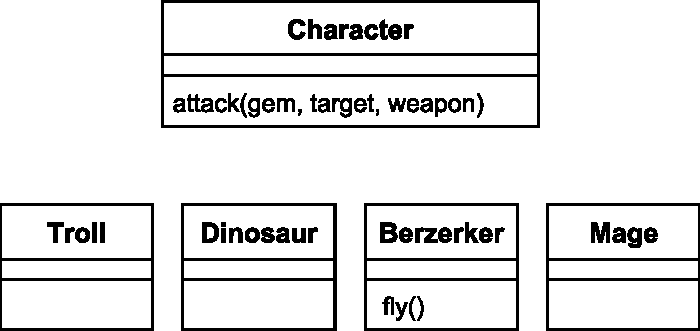
\includegraphics[width=\linewidth]{class_diagram_origin}
            \caption{original version (Jane's version)}
            \label{fig:class_diagram_origin}
        \end{subfigure}
        &
        \begin{subfigure}[t]{0.31\linewidth}
            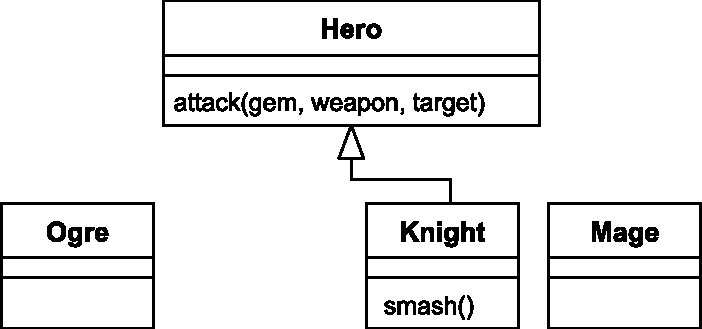
\includegraphics[width=\linewidth]{class_diagram_left}
            \caption{left version (Bob's version)}
            \label{fig:class_diagram_left}
        \end{subfigure}
        &
        \begin{subfigure}[t]{0.31\linewidth}
            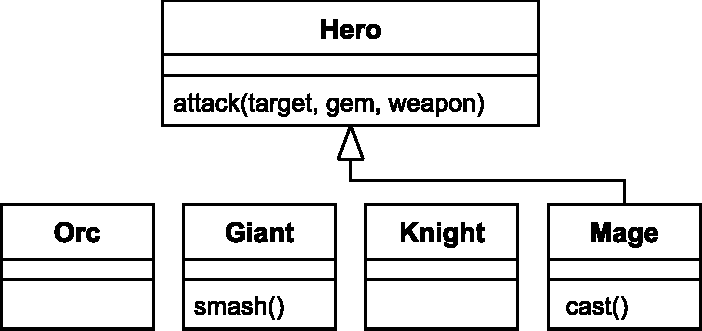
\includegraphics[width=\linewidth]{class_diagram_right}
            \caption{right version (Alice's version)}
            \label{fig:class_diagram_right}
        \end{subfigure}
    \end{tabular}
    \caption{Three class diagrams of a Role Playing Game.}
    \label{fig:class_diagram_rpg}
\end{figure*}

\section{Another Running Example}
\label{sec:another_running_example}
In this section, we introduce another running example to explain how to detect conflicts using the element tree. We use this example to construct a new element tree and to explain how conflict detection is performed in EMF Compare, EMF Store, and our change-based conflict detection. Let's say that there is a project to develop a Role Playing Game (RPG). Jane, as the technical leader, set up the initial model. The records of events during setting up the initial is recorded in the CBP in List. \ref{fig:class_diagram_origin}. From the List., we know that she created a class \textsf{Character} that contains an operation \textsf{attack} with three parameters: \textsf{gem}, \textsf{target}, and \textsf{weapon} (lines 1-14). She also created four other classes; \textsf{Troll} (lines 15-16), \textsf{Giant} (lines 17-21), \textsf{Knight} (lines 22-26), and \textsf{Mage} (lines 27-28). She then pushed her work to a change-based version control system. If her work is visualised in state-based format, the model looks like in Fig. \ref{fig:class_diagram_origin}.

\vspace{-15pt}
\begin{lstlisting}[firstnumber=1,style=eol,caption={The recorded events to produce the original model in Fig. \ref{fig:class_diagram_origin} (original version).},label=lst:cbp_origin]
create character type Class
set character.name to "Character" 
create attack type Operation
set attack.name to "attack" 
add attack to character.operations at 0
create gem type Parameter
set gem.name to "gem" 
add gem to attack.parameters at 0
create target type Parameter
set target.name to "target" 
add target to attack.parameters at 1
create weapon type Parameter
set weapon.name to "weapon" 
add weapon to attack.parameters at 2
create troll type Class
set troll.name to "Troll" 
create giant type class
set giant.name to "Giant"
create cast type Operation
set cast.name to "smash"
add cast to giant.operations at 0
create knight type Class
set knight.name to "Knight"
create smash type Operation
set smash.name to "smash"
add smash to knight.operations at 0
create mage type Class
set mage.name to "Mage" 
\end{lstlisting}

She then assigned this work to Bob and Alice. Both of them checked out this project to their own machine. Alice then started to continue the model. She then moved parameter \textsf{target} to the first place in operation \textsf{attack}'s parameters, because she thought it was more intuitive for programmers to think about the \textsf{target} first than the rest parameters (List. \ref{lst:cbp_right}, line 29). She also moved operations \textsf{smash} from class \textsf{Knight} to class \textsf{Giant} and \textsf{cast} from class \textsf{Giant} to class \textsf{Mage} as thy are more reasonable to belong to their new classes (lines 30-33). Alice also created a generalisation relationship with id \textsf{rightGen} from class \textsf{Troll} to class \textsf{Character} (34-36). Bob also did the same thing except that his generalisation came with id \textsf{leftGen} (List. \ref{lst:cbp_left}, line 29-31). 

Later on, Jane then informed them that she wanted all good characters should be derived from a general, hero-like class, and the enemy should be the Orcs not Trolls. She also instructed that Bob should focus on developing class \textsf{Knight} and Alice on class \textsf{Mage}. In consequence, Alice then changed the name of class \textsf{Character} from ``Character'' to ``Hero'' (the id of class \textsf{Hero} is still \textsf{character}) (line 37). Again, Bob did the same thing. He also changed the name of class \textsf{Character} from ``Character'' to ``Hero'' (line 32). Instead of creating a new generalisation relationship, both of them preferred to move the generalisation relationships that they had created to their assigned classes. Alice moved generalisation \textsf{rightGen} from class \textsf{Troll} to class \textsf{Mage} (lines 38-39), and Bob move generalisation \textsf{leftGen} from class \textsf{Troll} to class \textsf{Knight} (lines 33-34). Bob also moved parameter \textsf{target} in operation \textsf{attack} to the last index as he thought setting target as the last parameter was intuitive (line 35), and deleted the class {Giant}, and unfortunately, he deleted class \text{Giant} accidentally (lines 36-40). The class diagrams of Bob and Alice's models are visualised in Figures \ref{fig:class_diagram_left} and \ref{fig:class_diagram_right} respectively. Lastly, Alice changed the \textsf{name} of class \textsf{Troll} to ``Orc'' (line 40) while Bob changed it to ``Ogre'' (line 41).  

\vspace{-15pt}
\begin{lstlisting}[firstnumber=29,style=eol,caption={The appended events made by Alice to produce the right model in Fig. \ref{fig:class_diagram_right} (right version).},label=lst:cbp_right]
move target in attack.parameters from 1 to 0
remove smash from knight.operations at 0 composite l1
add smash to giant.operations at 0 composite l1
remove cast from giant.operations at 1 composite l2
add cast to mage.operations at 0 composite l2
create rightGen type Generalization
set rightGen.general to character
set troll.generalization to rightGen
set character.name from "Character" to "Hero"
remove rightGen from troll.generalization composite l3
set mage.generalization to rightGen composite l3
set troll.name from "Troll" to "Orc"
\end{lstlisting}

\vspace{-15pt}
\begin{lstlisting}[firstnumber=29,style=eol,caption={The appended events made by Bob to produce the left model in Fig. \ref{fig:class_diagram_left} (left version).},label=lst:cbp_left]
create leftGen type Generalization
set leftGen.general to character
set troll.generalization to leftGen
set character.name from "Character" to "Hero"
remove leftGen from troll.generalization composite r1
set knight.generalization to leftGen composite r1
move target in attack.parameters from 1 to 2
unset cast.name from "cast" to null composite r2
remove cast from giant.operations at 0 composite r2
delete cast composite r2
unset giant.name from "Giant" to null composite r2
delete giant comp r2
set troll.name from "Troll" to "Ogre"
\end{lstlisting}

In Listings \ref{lst:cbp_right} and \ref{lst:cbp_left}, we also introduce composite events -- lines with keyword \textsf{composite} -- that represent composite operations. Composite operations are operations that should be treated as one composition -- identified with the same composite id. For example, moving an element from a container to another container is composite event since it consists of two operations: removing/unsetting the element from its source container and adding/setting it to its target container (lines 36-37 Listing \ref{lst:cbp_right}). Using the information contained in CBPs in Listings in CBPs in Listings \ref{lst:cbp_right} and \ref{lst:cbp_left}, we can construct an element tree as depicted in Fig. \ref{fig:element_tree_game} using the element tree construction method presented in Section \ref{sec:tree_construction}.

\begin{figure*}
    \centering
    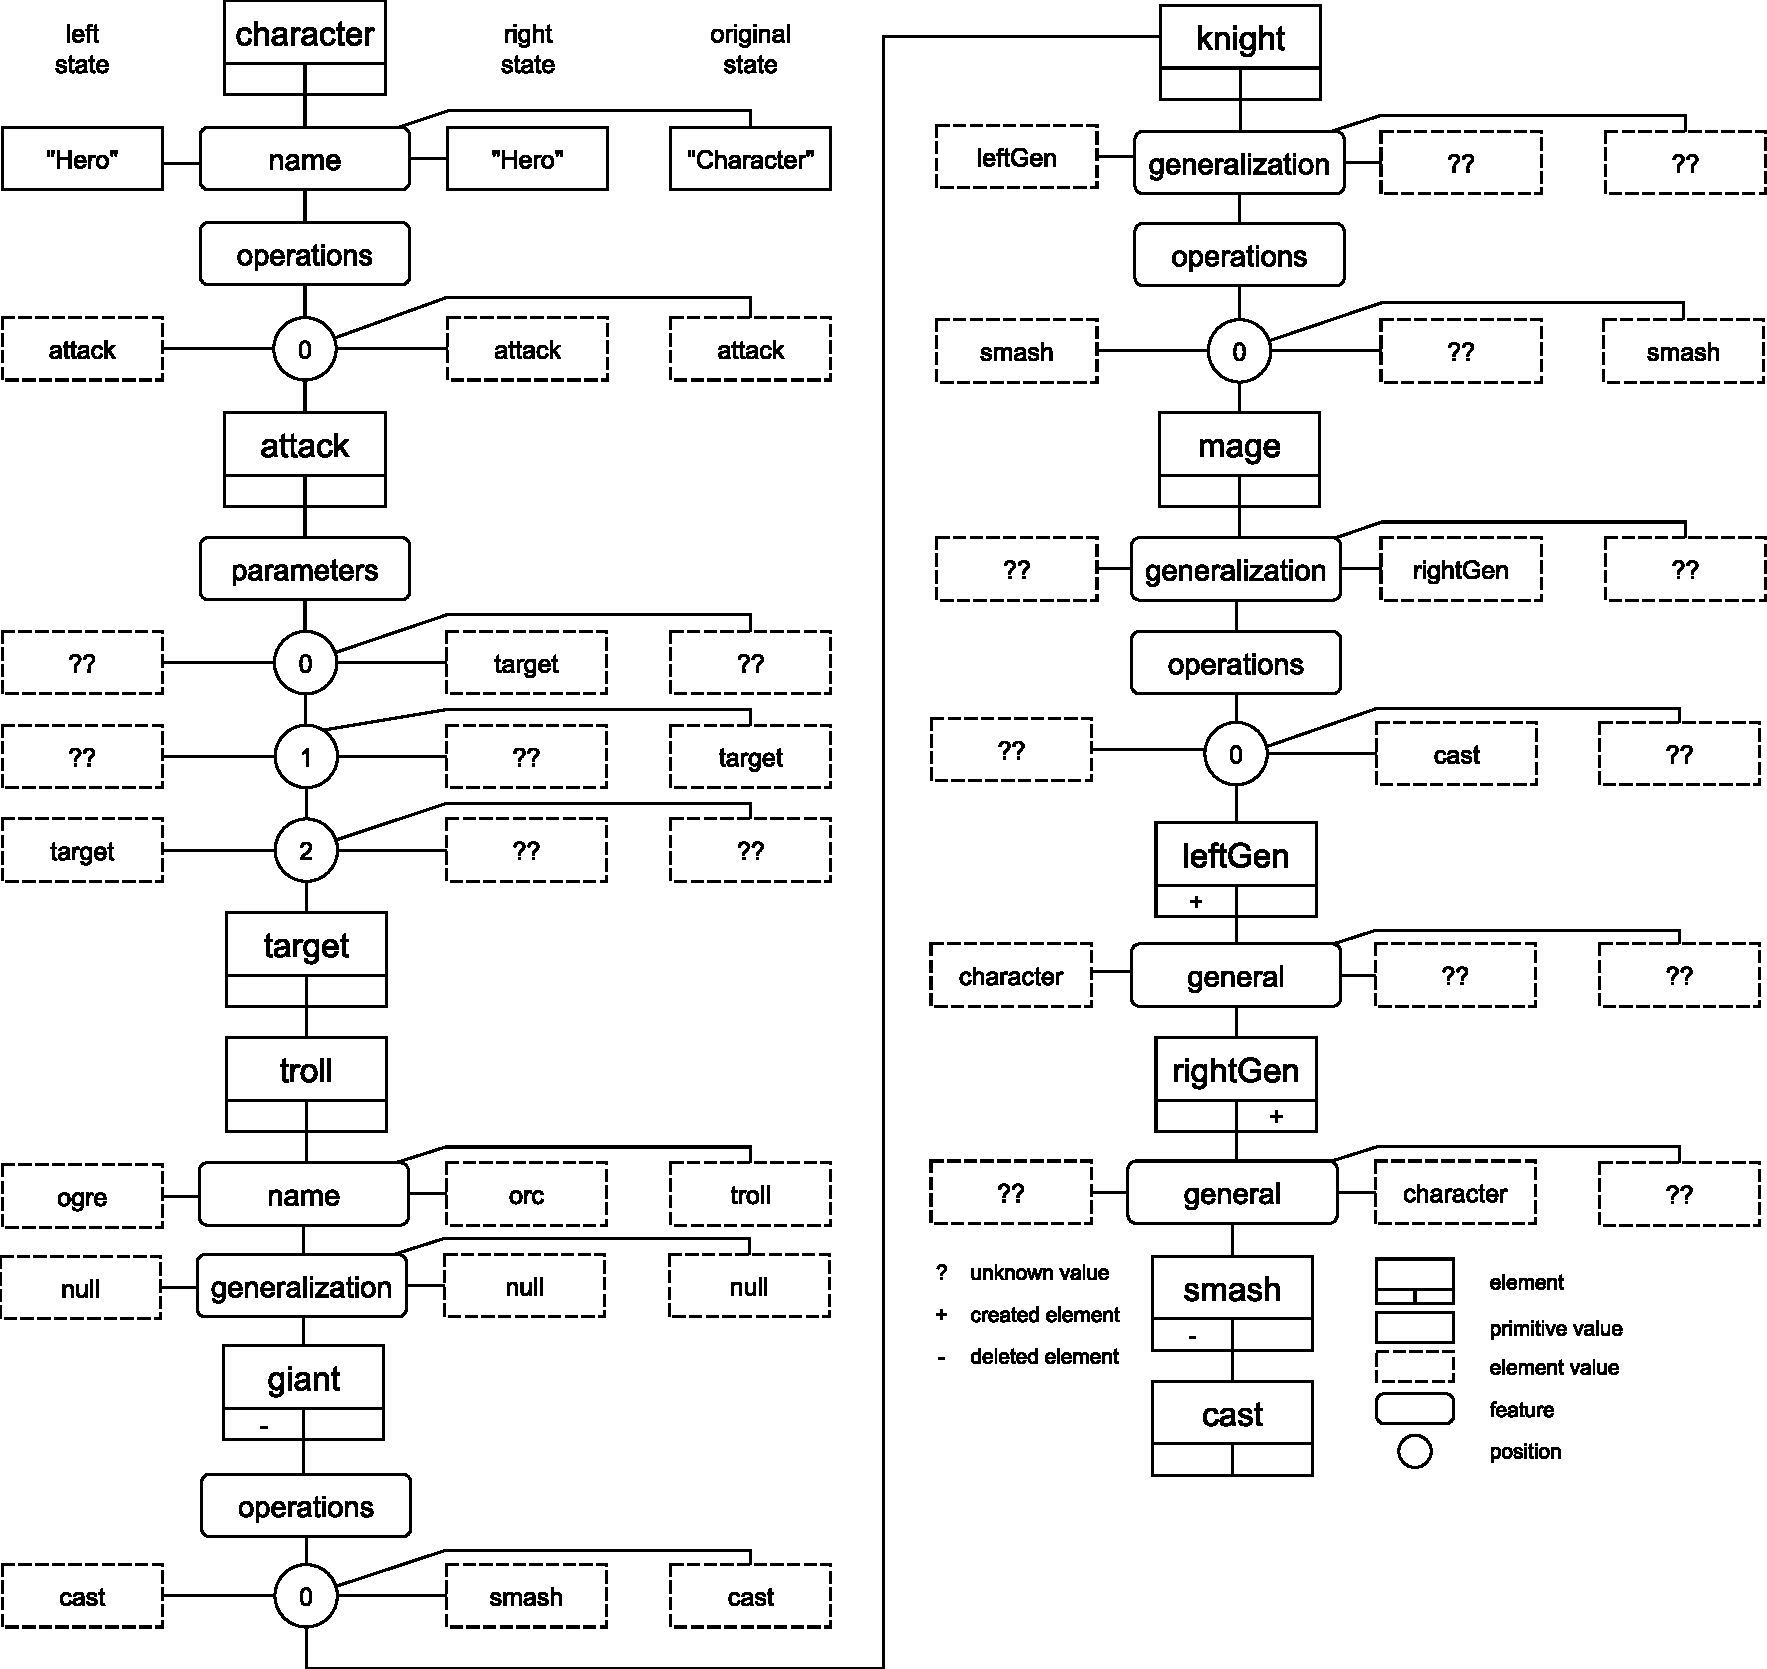
\includegraphics[width=\linewidth]{element_tree_game}
    \caption{An element tree constructed using information contained in CBPs in Listings \ref{lst:cbp_right} and \ref{lst:cbp_left}.}
    \label{fig:element_tree_game}
\end{figure*} 

\section{Conflict Detection}
\label{sec:conflict_detection}
In state-based model comparison, a conflict detection usually requires two different versions of a model and one shared ancestor -- the original version. In change-based model comparison, the original version is not required since it is implicitly contained in the other two versions' change-based persistence. A conflict occurs when an element is identified changed in both versions in reference to its original version. A conflict also occurs when a change from a version is applied first causes another change from the other version cannot be applied due to dependency violation. 

Let's say that we have three versions of a model: $m_{o}$ is the original version, $m_{l}$ is the left version, and $m_{r}$ is the right version, where $m_{o}$, $m_{l}$, $m_{r}$ $\in$ $M$. 
Every model consists of elements. Thus, $E_{O}$, $E_{L}$ , and $E_{R}$ are sets of elements of models $M_{O}$, $M_{L}$, and $E_{R}$ respectively, where $E_{O}=\{e_{o1}, e_{o2}, ..., e_{oa}\}$, $E_{L}=\{e_{l1}, e_{l2}, ..., e_{lb}\}$, and $E_{R}=\{e_{r1}, e_{r2}, ..., e_{rc}\}$. We also have two sets of operations $O_{L}$ and $O_{R}$ that changes model $m_{m}$ to models $m_{l}$ and $m_{r}$ respectively, where $O_{L}=\{o_{l1}, o_{l2}, ..., o_{ld}\}$ and $O_{R}=\{o_{r1}, o_{r2}, ..., o_{rf}\}$. 

\subsection{State-based Conflict Detection: EMF Compare}
\label{sec:state_based_conflict_detection_emf_compare}
In state-based model comparison, the two sets of operations $O_{L}$ and $O_{R}$ are not readily available. They have to be derived trough model differencing. Both sets can be obtained by differencing $M_{L}$ to $M_{O}$ and $M_{R}$ to $M_{O}$ using an LCS algorithm as explained in Section \ref{sec:model_differencing}. These two differencing processes produce two sets of differences, $D_{OL}$ and $D_{OR}$, where $D_{OL}$ = $\{d_{ol1}$, $d_{ol2}$, ..., $d_{olg}\}$, $D_{OR}$ = $\{d_{or1}$, $d_{or2}$, ..., $d_{orh}\}$, and each difference $d$ is expressed as in (\ref{eq:diff_definition}). These differences can be treated as operations since if we apply these differences as operations to a target model, they transform it to become equivalent to a reference model. For example, applying a set of differences $D_{OL}$ to a model $M_{O}$ will transform it to model $M_{L}$. Therefore, we can say that these differences are equivalent to operations. Thus, we can have two sets of operations, $O_{L}$ and $O_{R}$, which $O_{L} \equiv D_{OL}$ and $O_{R} \equiv D_{OR}$. These operations can then be used to detect conflicts using (\ref{eq:conflict_1.8}), (\ref{eq:conflict_1.9}), and (\ref{eq:conflict_1.10}).  

If we use EMF Compare to derive $O_{L}$ from Bob's and Jane's versions in Fig. \ref{fig:class_diagram_rpg} and present it in the format of change events, we obtain the following list. 
\begin{lstlisting}[firstnumber=1,style=eol,caption={The derived change events (operations) made by Bob to produce the right model in Fig. \ref{fig:class_diagram_left} (right version).},label=lst:cbp_left_state]
move target in attack.parameters from 1 to 2
set character.name from "Character" to "Hero"
set troll.name from "Troll" to "Ogre"
create leftGen type Generalization
set leftGen.general to character
set knight.generalization to leftGen
delete cast
delete giant
\end{lstlisting}

And following list is the derived change events for $O_{R}$ that are obtained from Bob's and Jane's versions in Fig. \ref{fig:class_diagram_rpg}. 
\begin{lstlisting}[firstnumber=1,style=eol,caption={The derived change events (operations) made by Alice to produce the right model in Fig. \ref{fig:class_diagram_right} (right version).},label=lst:cbp_right_state]
move gem in attack.parameters from 0 to 1
set character.name from "Character" to "Hero"
set troll.name from "Troll" to "Orc"
remove smash from knight.operations at 0
add smash to giant.operations at 0
create rightGen type Generalization
set rightGen.general to character
set mage.generalization to rightGen
remove cast from giant.operations at 1
add cast to mage.operations at 0
\end{lstlisting}

\textbf{Real Conflict}. In EMF Compare, a conflict occurs between two different operations, $o_{l}$ and $o_{r}$, if each is applied to a same element produce two different eventual states, where $!$ is the operator for expressing that two operations are in conflict. This conflict is classified \textsf{REAL} by EMF Compare.
\begin{equation} \label{eq:conflict_1.8}
e_{o} + o_{l} \not\equiv e_{o} + o_{r} \Rightarrow o_{l}\;!\;o_{r}
\end{equation} 
\textbf{Pseudo Conflict}. A conflict is classified as \textsf{PSEUDO} if the eventual states produced are equivalent. 
\begin{equation} \label{eq:conflict_1.9}
e_{o} + o_{l} \equiv e_{o} + o_{r} \Rightarrow o_{l}\;!_{p}\;o_{r}
\end{equation} 
\textbf{Non-applicability}. A conflict also occurs when applying operation $o_{l}$ to element $e_{o}$ makes $o_{r}$ inapplicable to element $e_{o}$. Therefore, operations $o_{l}$ and $o_{r}$ are in conflict. 
%For instance, Alice moved operation \textsf{smash} from class \textsf{Knight} to class \textsf{Giant} but this class was deleted by Bob. Deleting class \textsf{Giant} makes the move inapplicable. This conflict is classified \textsf{REAL} by EMF Compare.
\begin{equation} \label{eq:conflict_1.10}
(e_{o} + o_{r} \not\equiv e_{o}) \wedge (e_{o} + o_{l} + o_{r} \equiv e_{o} + o_{l}) \Rightarrow o_{l}\;!\;o_{r}
\end{equation}

\begin{table*}[]
    \centering
    \caption{Conflicting change events identified using EMF Compare based on the case in Fig. \ref{fig:class_diagram_rpg}.}
    \label{table:conflicts_emfc}
    % Please add the following required packages to your document preamble:
    % \usepackage[table,xcdraw]{xcolor}
    % If you use beamer only pass "xcolor=table" option, i.e. \documentclass[xcolor=table]{beamer}
    \begin{tabular}{|l|l|l|l|}
        \hline
        \multicolumn{1}{|c|}{{\color[HTML]{000000} \textbf{ID}}} & \multicolumn{1}{c|}{{\color[HTML]{000000} \textbf{Left Change Events (Bob)}}} & \multicolumn{1}{c|}{{\color[HTML]{000000} \textbf{Right Change Events (Alice)}}}                                      & \multicolumn{1}{c|}{{\color[HTML]{000000} \textbf{Type}}}           \\ \hline
        EC1                                                      & set character.name from "Character" to "Hero"                                 & set character.name from "Character" to "Hero"                                                                         & \begin{tabular}[c]{@{}l@{}}pseudo\\dual-state\end{tabular} \\ \hline
        EC2                                                      & set troll.name from "Troll" to "Ogre"                                         & set troll.name from "Troll" to "Orc"                                                                                  & \begin{tabular}[c]{@{}l@{}}dual-state\end{tabular}        \\ \hline
        EC3                                                      & delete cast                                                                   & \begin{tabular}[c]{@{}l@{}}remove smash from knight.operations at 0\\ add smash to giant.operations at 0\end{tabular} & \begin{tabular}[c]{@{}l@{}}non-\\ applicability\end{tabular}        \\ \hline
        EC4                                                      & delete giant                                                                  & \begin{tabular}[c]{@{}l@{}}remove cast from giant.operations at 1\\ add cast to mage.operations at 0\end{tabular}     & \begin{tabular}[c]{@{}l@{}}non-\\ applicability\end{tabular}        \\ \hline
    \end{tabular}
\end{table*}

Using (\ref{eq:conflict_1.8}), (\ref{eq:conflict_1.9}), and (\ref{eq:conflict_1.10}) and information in Listings \ref{lst:cbp_right_state} and \ref{lst:cbp_left_state}, we can identify four conflicts -- presented in Table \ref{table:conflicts_emfc} along with their conflicting change events. Conflict \textsf{EC1} is a pseudo duality conflict since both modify the same class \textsf{character}'s feature \textsf{name} resulting the same end states, ``Hero'' or ``Hero''. Conflict \textsf{EC2} is a duality conflict. Applying changing \textsf{troll}'s \textsf{name} to ``Ogre'' and \textsf{troll}'s \textsf{name} to ``Orc'' produces two different states -- ``Ogre'' and ``Orc''. Conflicts \textsf{EC3} and \textsf{EC4} are non-applicability conflicts since if we delete operation \textsf{cast} first then it cannot be added to class \textsf{giant}'s operations, and if we delete class \textsf{giant} first then operation \textsf{cast} cannot be added to that class' operations.

Conflict detection in state-based comparison might not be accurate since the derived differences/operations might not reflect the real historical changes of a model.
For example, EMF Compare does not detect that Alice and Bob modified the same element -- parameter \textsf{target} -- as indicated by line 29 in List. \ref{lst:cbp_right} and line 35 in List. \ref{lst:cbp_left} . Using an LCS algorithm, the derived operations related to the feature \textsf{parameters} of element \textsf{attack}, which if presented as change events, are expressed as [\texttt{\small \textbf{move} target \textbf{in} attack.parameters \textbf{from} 1 \textbf{to} 2}] for Bob's version and [\texttt{\small \textbf{move} gem \textbf{in} attack. parameters \textbf{from} 1 \textbf{to} 2}] for Alice's version. Using (\ref{eq:conflict_1.3}), both operations are not in conflict since both operations modify two different elements, \textsf{target} and \textsf{gem}. The result is different if we employ change-based approach to detect conflicts using the change event records in Listings \ref{lst:cbp_right} and \ref{lst:cbp_left}. We explain this in the next section, Section \ref{sec:change_based_conflict_detection_emf_store}.

%\begin{enumerate}
%    \item Operations/differences are determined using an LCS algorithm which might not reflect the real historical changes.
%    \item Two operations that modify a same element are perceived in conflict even though the end states after applying each operation are the same. 
%    \item When two operations on an element are in conflict. If one of the operation is selected as the applied operation, the other operation is only cancelled but the state of the element is not reversed back to its original state. This can cause an element does not exist after conflict resolution and merging.
%\end{enumerate}

%Drawbacks of EMF Store Conflict Detection and Resolution:
%\begin{enumerate} 
%    \item Two operations that modify a same element are perceived in conflict even though the end states after applying each operation are the same. This can lead to premature model after conflict resolution and merging since one of the two operation have to be reversed back even though there is no conflict.
%\end{enumerate}
%
%\begin{enumerate}
%    \item When two operations on an element are in conflict. If one of the operation is selected as the applied operation, the other operation is only cancelled but the state of the element is not reversed back to its original state. This can cause an element does not exist after conflict resolution and merging.
%    \item Operations/differences are determined using an LCS algorithm which might not reflect the real historical changes.
%    \item Two operations that modify an element are perceived in conflict even though the end states after applying each operation are the same. 
%\end{enumerate}

\subsection{Change-based Conflict Detection: EMF Store}
\label{sec:change_based_conflict_detection_emf_store}

\textbf{Non-commutability}. In EMF Store \cite{koegel2010emfstore} , operations $o_{l}$ and $o_{r}$ are in conflict if applying them in different order to a same element, in this case element $e_{o}$, produces two different eventual states.
\begin{equation} \label{eq:conflict_1.3}
e_{o} + o_{l} + o_{r} \not\equiv e_{o} + o_{l} + o_{r} \Rightarrow o_{l}\;!\;o_{r}
\end{equation} 
%For example, Alice changed the \textsf{name} of class \textsf{Troll} to ``Orc''while Bob renamed it to ``Ogre'' (Figure \ref{fig:class_diagram_rpg}). Applying Alice's change first to Bob's change results in the class' \textsf{name} equals to ``Ogre'', or ``Orc'' if the order is reversed. 
\textbf{Pseudo non-commutability}. However, after examining the implementation \footnote{\url{https://git.eclipse.org/c/emf-store}}, even though the eventual states are equivalent, both operations are still treated  in conflict. 
\begin{equation} \label{eq:conflict_1.5}
e_{o} + o_{l} + o_{r} \equiv e_{o} + o_{l} + o_{r} \Rightarrow o_{l}\;!_{p}\;o_{r}
\end{equation} 
\textbf{Non-applicability}. This non-applicability rule is the same with the non-applicability rule in the state-based conflict detection. We present the rule again here. 
\begin{equation} \label{eq:conflict_1.6}
(e_{o} + o_{r} \not\equiv e_{o}) \wedge (e_{o} + o_{l} + o_{r} \equiv e_{o} + o_{l}) \Rightarrow o_{l}\;!\;o_{r}
\end{equation}
\textbf{Composite}. If operation $o_{l}$ is in conflict with operation $o_{r}$ where $o_{r}$ is a member of composite operation $co_{r}$ then operation $o_{l}$ is also in conflict with each operation $o_{n}$ in composite operation $co_{r}$.
%For example, deleting class \textsf{Giant} (List. \ref{lst:cbp_left} line 40) is not only in conflict with adding operation \textsf{smash} to class \textsf{Giant}'s operations (List. \ref{lst:cbp_right} line 31), but also with the removal of operation \textsf{smash} from class \text{Knight}'s operations (List. \ref{lst:cbp_right} line 31).
\begin{equation} \label{eq:conflict_1.7}
o_{l}\;!\;o_{r} \wedge o_{r} \in co_{r} \Rightarrow o_{l}\;!\; \forall o_{n} | o_{n} \in co_{r}
\end{equation}

\begin{table*}[]
    \centering
    \caption{Conflicting change events identified using EMF Store in Listings \ref{lst:cbp_right} and \ref{lst:cbp_left}.}
    \label{table:conflicts_emfs}
    \begin{tabular}{|l|l|l|l|}
        \hline
        \multicolumn{1}{|c|}{{\color[HTML]{000000} \textbf{ID}}} & \multicolumn{1}{c|}{{\color[HTML]{000000} \textbf{Left Change Events (Bob)}}}                                                                                                                                              & \multicolumn{1}{c|}{{\color[HTML]{000000} \textbf{Right Change Events (Alice)}}}                                                          & \multicolumn{1}{c|}{{\color[HTML]{000000} \textbf{Type}}}                                    \\ \hline
        \multirow{2}{*}{ES1} & set troll.generalization from null to leftGen                                                                                                                                                                              & \begin{tabular}[c]{@{}l@{}}unset troll.generalization from rightGen to null\\set mage.generalization from null to rightGen\end{tabular} & \multirow{2}{*}{\begin{tabular}[c]{@{}l@{}}non-\\ commutability, \\ composite\end{tabular}}                                                                                             \\ \cline{2-3}
                                            & \begin{tabular}[c]{@{}l@{}}unset troll.generalization from leftGen to null\\ set knight.generalization from null to leftGen\end{tabular}                                                                                   & set troll.generalization from null to rightGen                                                                                             &  \\ \hline
        ES2                                                      & set character.name from "Character" to"Hero"                                                                                                                                                                               & set character.name from "Character" to "Hero"                                                                                             & \begin{tabular}[c]{@{}l@{}}pseudo non-\\ commutability\end{tabular}                          \\ \hline
        ES3                                                      & move target in attack.parameters from 1 to 2                                                                                                                                                                               & move target in attack.parameters from 1 to 0                                                                                              & \begin{tabular}[c]{@{}l@{}}non-\\ applicability\end{tabular}                                 \\ \hline
        \multirow{2}{*}{ES4} & \multirow{2}{*}{\begin{tabular}[c]{@{}l@{}}unset cast.name from "cast" to null\\ remove cast from giant.operations at 0\\ delete cast type Operation\\ unset giant.name from "Giant" to null\\ delete giant\end{tabular}}                                                                                                                                                                                                                            & \begin{tabular}[c]{@{}l@{}}remove cast from giant.operations at 0\\ add cast to mage.operations at 0 \end{tabular}                         
        & \multirow{2}{*}{\begin{tabular}[c]{@{}l@{}}non-\\ applicability,\\ composite\end{tabular}} \\ \cline{3-3}
        &  & \begin{tabular}[c]{@{}l@{}}remove smash from knight.operations at 0\\ add smash to giant.operations at 1\\ \\ \\ \end{tabular}                     &   \\ \hline
        
        ES5                                                      & set troll.name from "Troll" to "Ogre"                                                                                                                                                                                      & set troll.name from "Troll" to "Orc"                                                                                                      & \begin{tabular}[c]{@{}l@{}}non-\\ commutability\end{tabular}                                 \\ \hline
    \end{tabular}
\end{table*}

In change-based conflict detection, all operations applied to a model are already available in change-based persistence, thus the operations do not need to be derived trough a diffing process. The availability of real historical changes can improve the accuracy of change detection since we can identify precisely elements that have been changed. In consequence, the undetected conflict in state-based conflict detection can be detected. For example, in Listing \ref{lst:cbp_right} line 29, parameter \textsf{target} has been moved from index 1 to 0, while in Listing \ref{lst:cbp_left} line 35, it was moved from index 1 to 2. Since both operations modified the same parameter \textsf{target}, using (\ref{eq:conflict_1.3}) we can identify that both operations are in conflict; parameter \textsf{target} are at different indexes if both operations are applied in different order, and \textsf{parameters}, the containing feature of \textsf{target}, is an ordered feature (Table \ref{table:conflicts_emfs} id ES1).  

The drawback of EMF Store is that it only performs comparison between operations to determine conflicts; it does no take into account the end states of models produced by the operations. In consequence, two operations are in conflict just by modifying a same element regardless of the end states that they produce to the element \cite{DBLP:conf/sfm/BroschKLSWW12}; there is no classification of conflicts to \textsf{REAL} or \textsf{PSEUDO} conflicts. For example, two operations represented by the two change events in Listing \ref{lst:cbp_right} at line 37 and Listing \ref{lst:cbp_right} at line 32, that change the same feature \textsf{name} to the same value ``Hero'', are treated in conflict (Table \ref{table:conflicts_emfs} id ES2). 

The inconsideration of eventual states also causes the assignments of generalizations \textsf{leftGen} and \textsf{rightGen} to class \textsf{troll}'s feature \textsf{generalization}, in Listings \ref{lst:cbp_right} at line 38 and \ref{lst:cbp_left} at line 33, to be in conflict with the \textsf{move} operations on the opposite sides (Table \ref{table:conflicts_emfs} id ES1). Setting feature \textsf{troll}'s \textsf{generalization} to element \textsf{leftGen} is in conflict with the \textsf{move} composite operation that moves \textsf{rightGen} from \textsf{troll}'s \textsf{generalization} to \textsf{mage}'s \textsf{generalization}. Using the non-commutability (\ref{eq:conflict_1.3}) and composite (\ref{eq:conflict_1.7}) rules, we can detect that executing these operations in different order causes \textsf{troll}'s \textsf{generalization} has two different eventual values; \textsf{troll}'s \textsf{generalization} is null if the \textsf{move} operation is executed first or \textsf{leftGen} if the \textsf{set} operation is executed first. We can use the same reasoning to explain the conflict between setting feature \textsf{troll}'s \textsf{generalization} to element \textsf{rightGen} and the \textsf{move} composite operation that moves \textsf{leftGen} from \textsf{troll}'s \textsf{generalization} to \textsf{knight}'s \textsf{generalization}.

In state-based conflict detection, the latter case (ES1) is not a conflict since the values of class \textsf{troll}'s feature \textsf{generalization} in the Jane's, Bob's, and Alice's versions are indentical -- all are null. Thus, there are no \textit{derived} operations that concurrently modify class \textsf{troll}'s feature \textsf{generalization}. Conflict ES4 is a non-applicability, composite conflict. Moving element \textsf{smash} from class \textsf{knight} to class \textsf{giant} and moving element \textsf{cast} from class \textsf{giant} to class \textsf{mage} require the deletion of class \textsf{giant} to be executed later in order to be applicable. Conflict ES5 is a non-commutability conflict. The \text{name} of class \textsf{troll} have an eventual value ``Ogre'' or ``Orc'' depending on the execution order of the conflicting operations.

\section{Change-based Conflict Detection: Epsilon CBP}
\label{change_based_conflict_detection_epsilon_cbp}

In our conflict detection, we take two strategies from both change and state-based conflict detections to improve the accuracy of our approach. We exploit change events to accurately address real historical changes -- not derived ones -- of models. We also take into account the eventual states of models being compared. Thus, two sequences of operations that produce two equivalent eventual states should not be treated in conflict. For the latter strategy, the eventual states is already calculated during the construction of the \textsf{element tree}. Since we also registered change events to every element and feature involved, we can obtain all related change events that produce the eventual state of an element or feature. Let's say that we have the original state of an element $e_{o}$. We also have a set of operations $O_{L}$ = $\{$$o_{l1}$, $o_{l2}$$\}$ that we apply to $e_{o}$ that changes its state to element $e_{l}$. 
\begin{equation} \label{eq:conflict_3.1}
e_{o} + o_{l1} + o_{l2} \rightarrow e_{l}
\end{equation} 
Moreover, we also have another set of operations $O_{R}$ = $\{$$o_{r1}$, $o_{r2}$$\}$ that we apply to $e_{o}$ that produces element $e_{r}$.
\begin{equation} \label{eq:conflict_3.2}
e_{o} + o_{r1} + o_{r2} \rightarrow e_{r}
\end{equation} 
Instead of calculating conflict between operations, we start by checking the equivalency of the states of an element on both sides. If the states on both sides are equivalent then we can argue that there is no conflict between operations that produce both equal states, $e_{l}$ and $e_{r}$. 
\begin{equation} \label{eq:conflict_3.3}
e_{l} \equiv e_{r} \Rightarrow \neg(\exists o_{l} \in O_{L} \;!\; \exists o_{r} \in O_{R})
\end{equation} 
Therefore, we can also argue that if both states, $e_{l}$ and $e_{r}$, are not equivalent and, at least, there is an operation applied to the element on each side then it can be concluded that there is, at least, one operation of operations $O_{L}$ that is in conflict with, at least, one operation of the operations $O_{R}$. 
\begin{equation} \label{eq:conflict_3.10}
\begin{split}
& e_{l} \not\equiv e_{r} \wedge |O_{L}| > 0 \wedge |O_{R}| > 0 \Rightarrow\\
& \exists o_{l} \in O_{L} \;!\; \exists o_{r} \in O_{R}
\end{split}
\end{equation} 
Such calculation is possible since in every element or feature we record all operations that affect them during the construction of the element tree. 


\IncMargin{1.5em}
\begin{algorithm*}
    \begin{footnotesize}
        \SetKwInOut{Input}{input}
        \SetKwInOut{Output}{output}
        \Input{an instance of ElementTree $elementTree$}
        \Begin{
            $conflictList$ $\leftarrow$ ConflictList()\;
            \ForEach{$element$ \In $elementTree$}{
                \If{isLeftDeleted($element$) \Or isRightDeleted($element$)}{
                    $leftEvents$ $\leftarrow$ getAllRelatedLeftEvents($element$)\;
                    $rightEvents$ $\leftarrow$ getAllRelatedRightEvents($element$)\;
                    \If{size($leftEvents$) > 0 \AndA size($rightEvents$) > 0}{
                        $conflict$ $\leftarrow$ createConflict($leftEvents$, $rightEvents$)\;
                        addConflict($conflict$, $conflictList$)\;
                    }
                }
                \If{getLeftContainer($element$) <> getRightContainer($element$) \Or getLeftContainingFeature($element$) <> getRightContainingFeature($element$)}{
                    $leftEvents$ $\leftarrow$ getAllRelatedLeftEvents($element$)\;
                    $rightEvents$ $\leftarrow$ getAllRelatedRightEvents($element$)\;
                    \If{size($leftEvents$) > 0 \AndA size($rightEvents$) > 0}{
                        $conflict$ $\leftarrow$ createConflict($leftEvents$, $rightEvents$)\;
                        addConflict($conflict$, $conflictList$)\;
                    }
                }
                \ForEach{$feature$ \In getFeatures($element$)}{
                    \uIf{isSingleValued($feature$)}{
                        $leftEvents$ $\leftarrow$ getAllRelatedLeftEvents($element$, $feature$)\;
                        $rightEvents$ $\leftarrow$ getAllRelatedRightEvents($element$, $feature$)\;
                        \If{size($leftEvents$) > 0 \AndA size($rightEvents$) > 0}{
                            $conflict$ $\leftarrow$ createConflict($leftEvents$, $rightEvents$)\;
                            addConflict($conflict$, $conflictList$)\;
                        }
                    }\ElseIf{isMultiValued($feature$)}{
                        \uIf{isOrdered($feature$)}{
                            $values$ $\leftarrow$ getUnequalLeftAndRightValues($feature$)\;
                            \ForEach{$value$ \In $values$}{
                                $leftEvents$ $\leftarrow$ getAllRelatedLeftEvents($element$, $feature$, $value$)\;
                                $rightEvents$ $\leftarrow$ getAllRelatedRightEvents($element$, $feature$, $value$)\;
                                \If{size($leftEvents$) > 0 \AndA size($rightEvents$) > 0}{
                                    $conflict$ $\leftarrow$ createConflict($leftEvents$, $rightEvents$)\;
                                    addConflict($conflict$, $conflictList$)\;
                                }       
                            }
                        }\ElseIf{\Not isOrdered($feature$)}{
                            $values$ $\leftarrow$ getXORLeftAndRightValues($feature$)\;
                            \ForEach{$value$ \In $values$}{
                                $leftEvents$ $\leftarrow$ getAllRelatedLeftEvents($element$, $feature$, $value$)\;
                                $rightEvents$ $\leftarrow$ getAllRelatedRightEvents($element$, $feature$, $value$)\;
                                \If{size($leftEvents$) > 0 \AndA size($rightEvents$) > 0}{
                                    $conflict$ $\leftarrow$ createConflict($leftEvents$, $rightEvents$)\;
                                    addConflict($conflict$, $conflictList$)\;
                                }       
                            }
                        }
                    }
                }
            }
            \Return{$conflictList$}\;
        }
    \end{footnotesize}
    \caption{Algorithm for conflict detection using element tree.}
    \label{alg:conflict_detection}
\end{algorithm*}
\DecMargin{1.5em}


\begin{table*}[]
    \centering
    \caption{Conflicting change events in Listings \ref{lst:cbp_right} and \ref{lst:cbp_left} identified using our proposed conflict detection.}
    \label{table:conflicts_cbp}
    \begin{tabular}{|l|l|l|l|}
        \hline
        \multicolumn{1}{|c|}{{\color[HTML]{000000} \textbf{ID}}} & \multicolumn{1}{c|}{{\color[HTML]{000000} \textbf{Left Change Events (Bob)}}}                                                                                                                            & \multicolumn{1}{c|}{{\color[HTML]{000000} \textbf{Right Change Events (Alice)}}}                                                                                                                  & \multicolumn{1}{c|}{{\color[HTML]{000000} \textbf{Type}}}                 \\ \hline
        CB1                                                      & set troll.name from "Troll" to "Ogre"                                                                                                                                                                    & set troll.name from "Troll" to "Orc"                                                                                                                                                              & \begin{tabular}[c]{@{}l@{}}non-\\ commutability\end{tabular}              \\ \hline
        CB2                                                      & move target in character.parameters from 1 to 2                                                                                                                                                          & move target in character.parameters from 1 to 0                                                                                                                                                   & \begin{tabular}[c]{@{}l@{}}non-\\ commutability\end{tabular}              \\ \hline
        CB3                                                      & \begin{tabular}[c]{@{}l@{}}unset cast.name from "cast" to null\\ remove cast from giant.operations at 0\\ delete cast type Operation\\ unset giant.name from "Giant" to null\\ delete giant\end{tabular} & \begin{tabular}[c]{@{}l@{}}remove cast from giant.operations at 0\\ add cast to mage.operations at 0\\ remove smash from knight.operations at 0\\ add smash to giant.operations at 1\end{tabular} & \begin{tabular}[c]{@{}l@{}}non-\\ applicability,\\ composite\end{tabular} \\ \hline
    \end{tabular}
\end{table*}

 
\section{Evaluation Method}
\label{sec:evaluation}
In this section, we present the method that we employed to evaluate our change-based comparison approach and discuss the results. We also present the limitations and threats to the validity of the evaluation.

In order to assess the performance benefits of the change-based approach in terms of model comparison -- differencing and conflict detection, we have evaluated it against a mature and widely-used state-based comparison tool (EMF Compare \cite{emfcompare2018developer,eclipse2017compare}). Since there are no manually developed, large models persisted in our change-based format yet, the dataset for our experiments was constructed from a large model reverse-engineered from the Eclipse Epsilon project \cite{eclipse2018epsilongit,eclipse2017epsilon}. This model conforms to the Java metamodel \cite{eclipse2018modiscojava} and consists of more than 1.6 million elements with a size of 224 MBs when persisted in XMI. 

We cloned the original model to produce two new (left and right) models and perform operations (\textsf{add}, \textsf{remove}, \textsf{move}, \textsf{set} with random elements, features, indexes, and values) on both models to create differences. We made 1.1 million artificial changes to each model, generating over 1.1 million events (one operation can generate more than one event, e.g. a \textsf{move} between features generates \textsf{remove} and \textsf{add} events). Events generated by the changes were persisted in our change-based format (to be used later in change-based model comparison). After every 50,000 changes, we made a measurement point. We persisted the last state of the models in state-based format (to be used later in state-based model comparison) and then performed change-based and state-based model comparison and measured their execution time and memory footprint. We created 22 measurement points to capture their trends in one experiment. 

\subsection{Model Differencing}
\label{sec:differencing_evaluation}

We conducted five experiments to evaluate the model differencing of our approach.
%batches \dk{Would it make sense to call these ``experiments'' instead? i.e. ``We conducted five experiments. In the first experiment \ldots''}. 
In the first experiment, the ratio of occurrence between \textsf{add}, \textsf{remove}, \textsf{move}, and \textsf{set} changes is set to 1:1:20:40 intuitively in assumption that in a mature model modification -- \textsf{move} and \textsf{set} events -- occurs more frequent than addition and deletion. Since we wanted the change of total elements not to affect our measurement, the number of total elements should be kept constant. For example, it is difficult to tell an increase of time in comparison is caused by an increase in the number of elements or by the number of change events. One way to do this was to exclude \textsf{add} and \textsf{remove} operations. However, excluding both operations made measurement less representative. Thus, we still included both operations but made their probabilities equal so that the number of total elements remain largely unchanged. In the rest of the experiments,
%batches \dk{Replace with ``In the remaining four experiments''? - it may not be entirely clear to the reviewers what ``to support'' means in this context}
we only performed homogeneous type operations -- isolated from other types -- per experiment (e.g. add-only, move-only operations). In the end, we obtained 5 results of the experiments: mixed, add-only, remove-only, move-only, and set-only measurement results. We did this to asses whether operations of different types have a different impact on model comparison.
%\dk{Explain that we did this to assess whether events of different types have a different impact on model comparison?}

For the change-based approach, the comparison time comprises loading change events, constructing an element tree, and identifying differences. The memory footprint is the space used to hold the change events, element tree, and differences in memory. For the state-based approach, the comparison time comprises matching elements and identifying differences, and the memory footprint is the space required to hold the matches and differences in memory. All measurements were performed on the same machine with the following specification: AMD Opteron(tm) Processor 6386 SE @ 2.8 GHz cache size 2 GBs (64 processors), 528 GBs main memory, Ubuntu 16.04.6 LTS operating system, and Java(TM) SE Runtime Environment (build 1.8.0\_201-b09) with JVM \textsf{InitialHeapSize} 2GBs and \textsf{MaxHeapSize} 32 GBs.
%\dk{Add the spec of the machine + the version of Java used + how much memory was allocated to the JVM}

Since the change-based and state-based approaches can produce a different number of syntactically equivalent differences, in order to evaluate the correctness of the change-based approach, we reconciled all the differences by performing all-left-to-right merging -- making the right model identical to the left model -- based on the identified differences. If the all-left-to-right merging of change-based approach produces a model that is identical to the model produced by the all-left-to-right merging of the state-based approach then it can be said that differences identified by the change-based approach are correct. We performed this correctness checking at every measurement point.

\subsection{Conflict Detection}
\label{sec:conflict_detection_evaluation}
In evaluating our conflict detection approach, basically we followed the similar procedures as in the model differencing evaluation, except that we add another implementation of change-based model persistence (EMF Store \cite{koegel2010emfstore}) to compare it with our approach. We did not include it in the model differencing evaluation since it works purely on operations, and it is designed to identify conflict between operations; not for finding differences between models. We imported the changes persisted in our change-based format into EMF Store by replaying the changes in the EMF Store. Thus, we could obtained the same changes but in the EMF Store format. Since in this evaluation we used two change-based persistence: our approach and EMF Store, we use the term Epsilon CBP to refer to our approach.

\begin{figure*}
    \vspace{-26pt}
    \begin{subfigure}[t]{0.33\linewidth}
    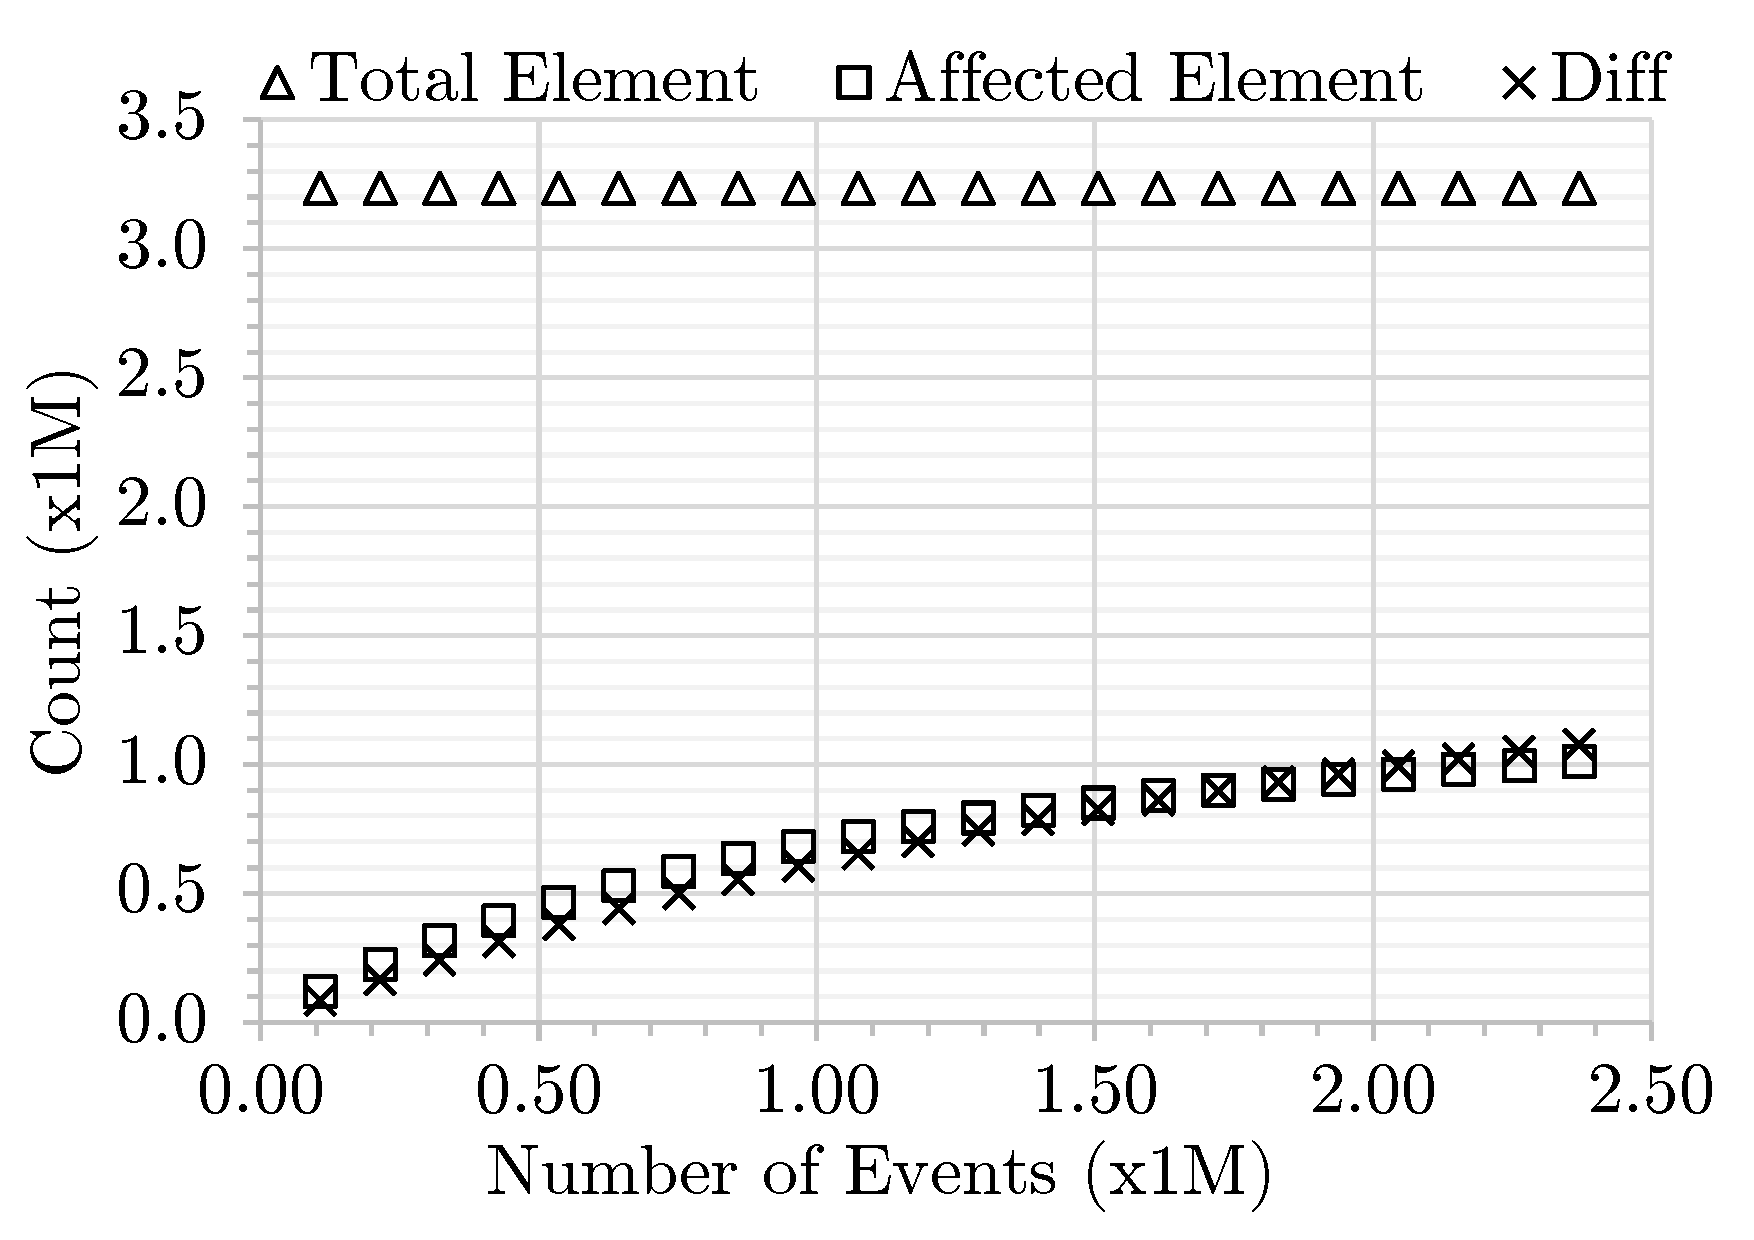
\includegraphics[width=\linewidth]{mixed-count-events}
    \caption{total elements, affected elements, and diffs}
    \label{fig:modification_course}
    \end{subfigure}
    \begin{subfigure}[t]{0.33\linewidth}
        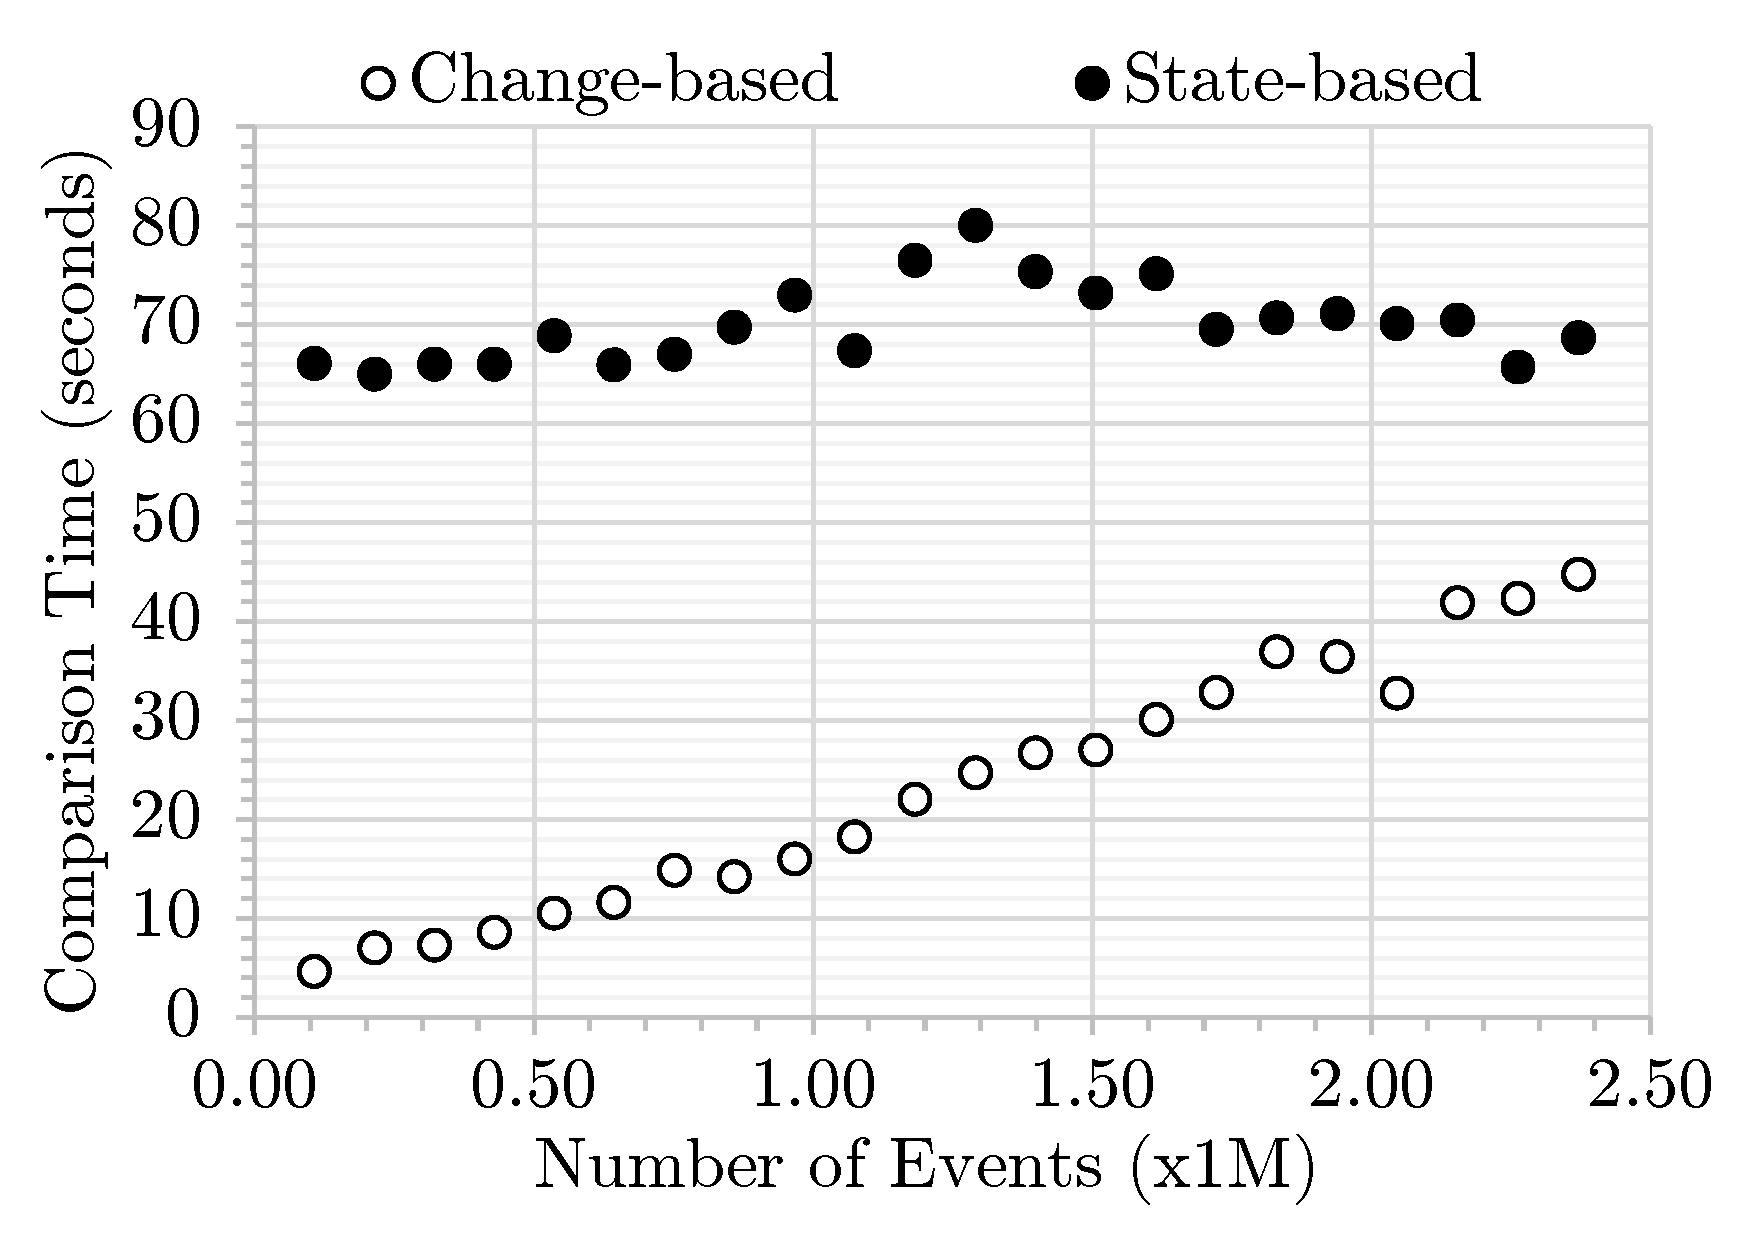
\includegraphics[width=\linewidth]{mixed-time-events}
        \caption{execution time}
        \label{fig:time_diffs}
    \end{subfigure}
    \begin{subfigure}[t]{0.33\linewidth}
        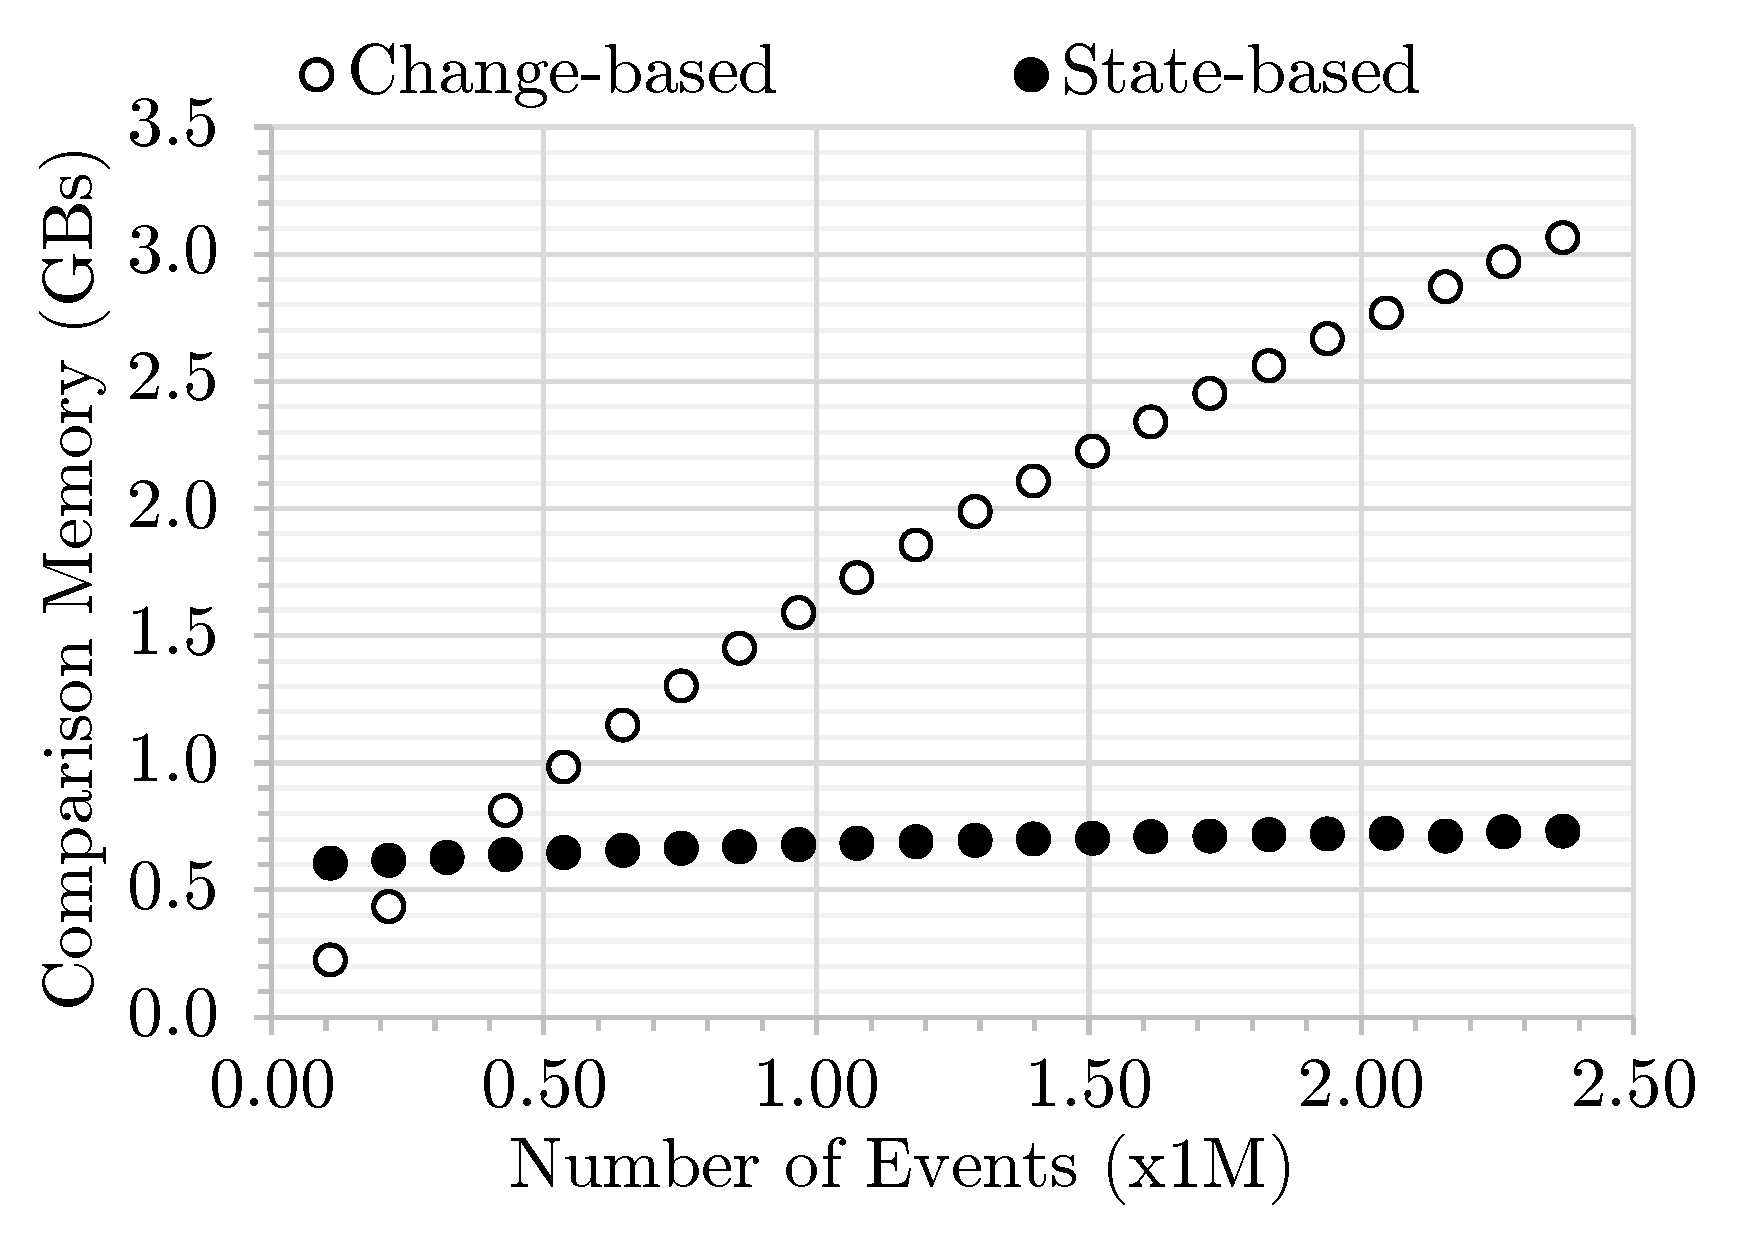
\includegraphics[width=\linewidth]{mixed-memory-events}
        \caption{memory footprint}
        \label{fig:memory_diffs}
    \end{subfigure}
    \caption{Change-based vs. state-based model comparison as change events increase.}
    \label{fig:change_vs_state}
\end{figure*}

\vspace{-5pt}
\section{Results and Discussion}
\label{sec:discussion}
In this section, we report on the obtained results in terms of comparison time and memory footprint for both model differencing and conflict detection. 


\subsection{Model Differencing}
\label{sec:differencing_results}
This section presents the results of both mixed and homogeneous operation measurements for the model differencing evaluation. 

\vspace{-5pt}
\subsubsection{Mixed Operations} \label{sec:mixed-operation}

In the mixed operation measurement, we modify two identical models differently by applying random operations. As the number of change events generated by the modification grows, the numbers of affected elements and differences also increase in a logarithmic manner. The patterns can be seen in Fig. \ref{fig:modification_course}. The growth is logarithmic since the probability that the random operations modify the same elements also increases. Thus, some change events might not contribute to the addition of new affected elements and differences. In other words, more events are required to increase the number of affected elements or differences. In Fig. \ref{fig:modification_course}, the total elements remains largely unchanged due to the equal probabilities of addition and deletion as has been set in Section \ref{sec:evaluation}. The figure gives us an insight about the characteristics of the modification caused by the random operations in the mixed operation measurement; it supports explaining the implication of the changes on execution time and memory footprints of model comparison.

After applying some random changes on both models, the modification produces 100,000 change events at the first measurement point. Using this amount of events, our change-based comparison only takes 5 seconds to identify around 90,000 differences, in contrast to the state-based comparison that takes 66 seconds (see the first measurement points in Figures \ref{fig:modification_course} and \ref{fig:time_diffs}). If the modification continues, more changes events are generated. This growing number of change events has to be loaded into memory and thus slows down the change-based comparison. Nevertheless, the change-based comparison is still faster than the state-based comparison even though the number of change events reaches 2.37 millions -- more than 1 million differences at that point; the change-based comparison outperforms the state-based comparison in execution time (Figure \ref{fig:time_diffs}). Fig. \ref{fig:time_changediff_detail} breaks down the comparison time in detail. It exhibits that the event loading time is the dominant contributor to the slowdown compared to the element tree's construction time and diffing time. 

\begin{figure*}[ht]
    \centering
    \begin{subfigure}[t]{0.245\linewidth}
        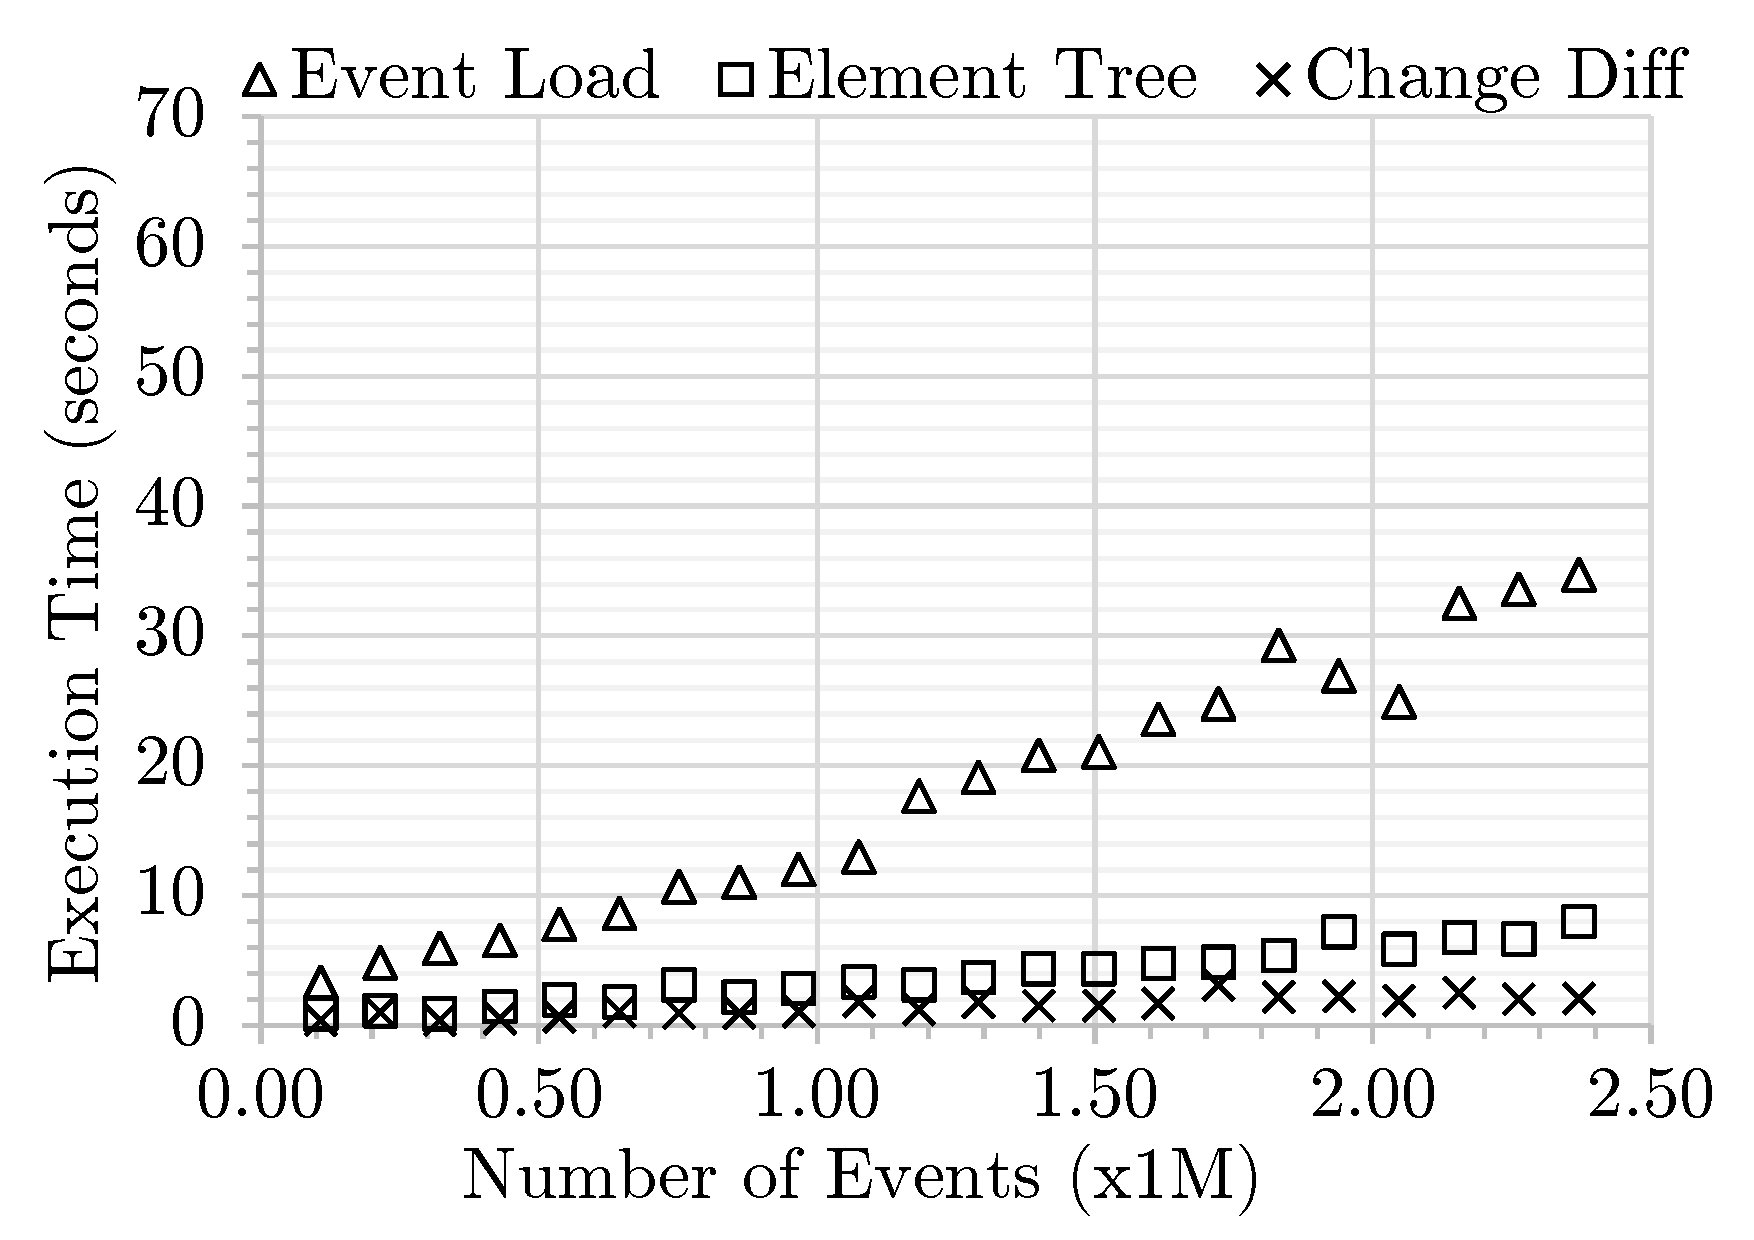
\includegraphics[width=\linewidth]{mixed-time-events-detail}
        \caption{change-based comparison time}
        \label{fig:time_changediff_detail}
    \end{subfigure}
    \hfill
    \begin{subfigure}[t]{0.245\linewidth}
        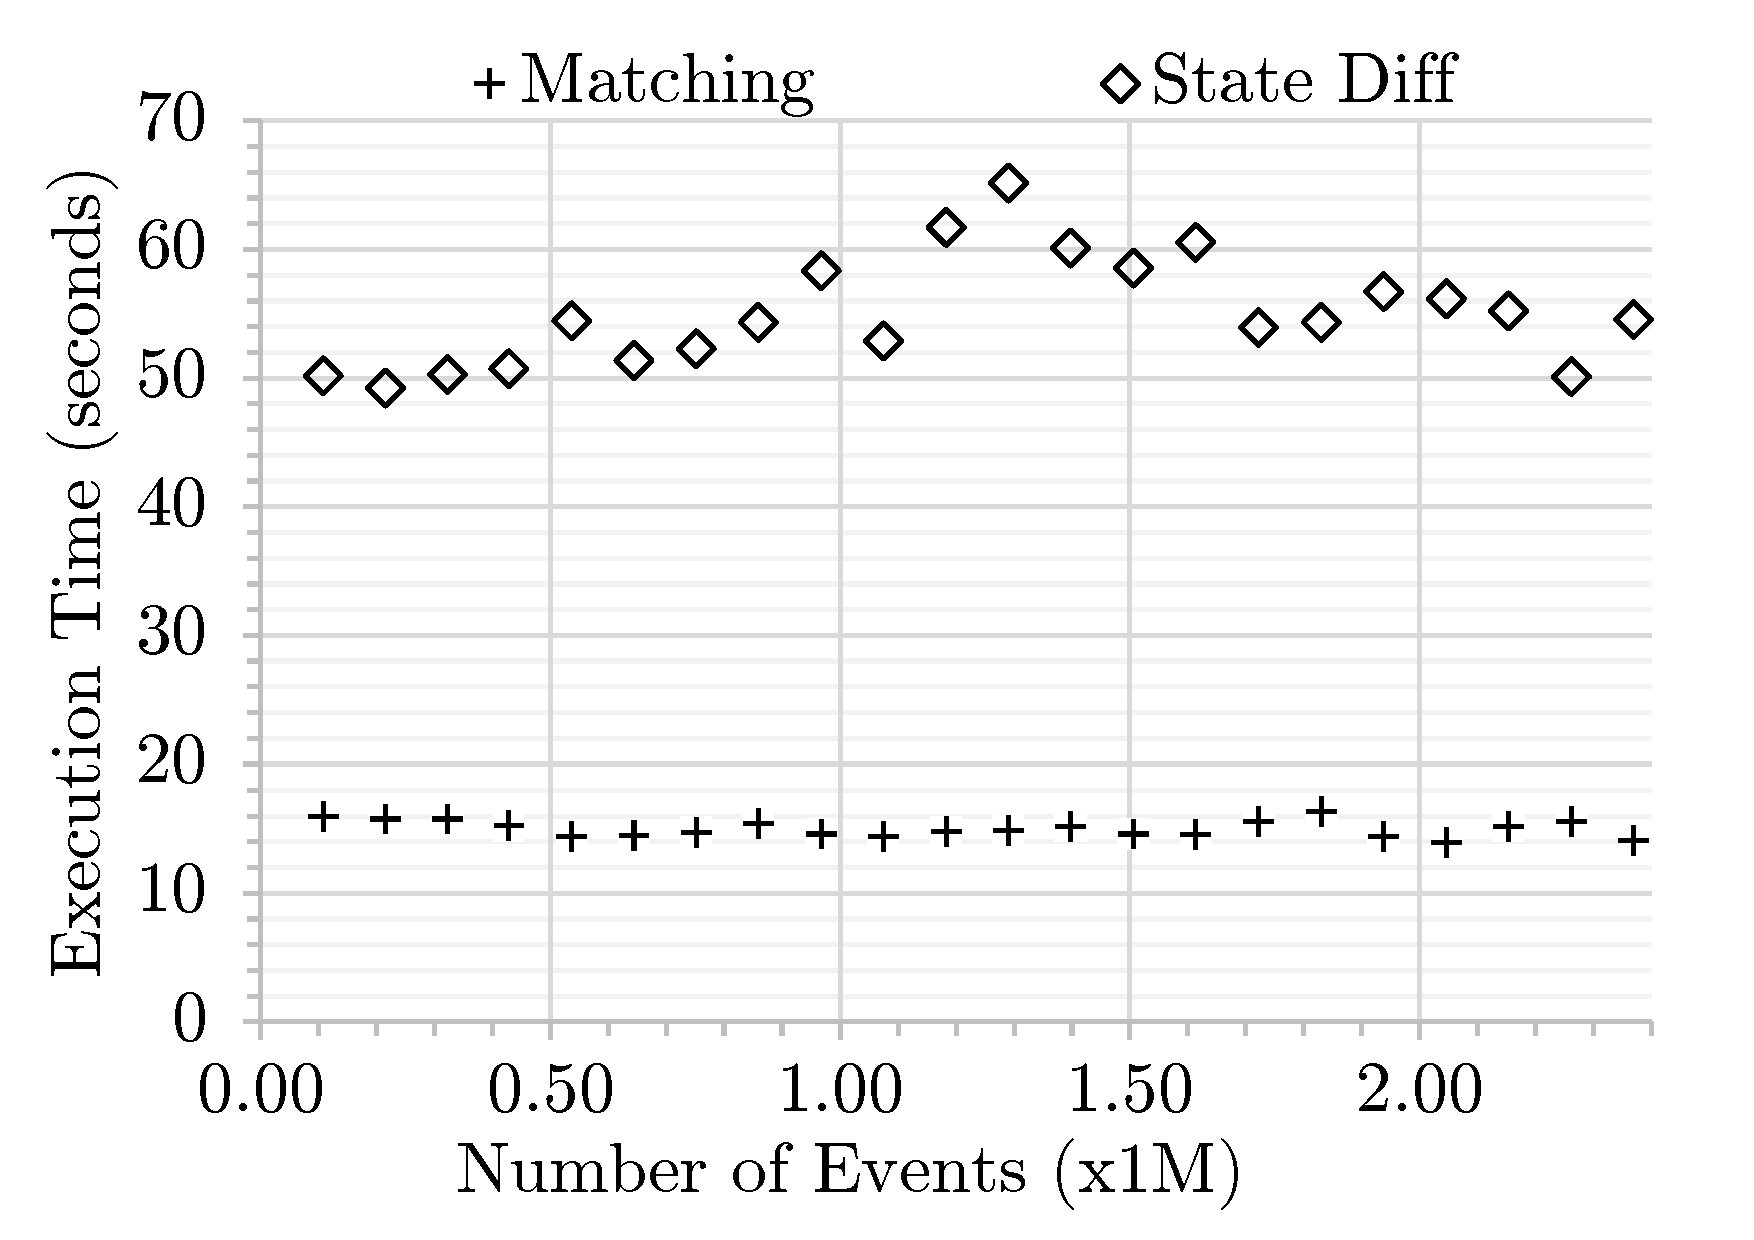
\includegraphics[width=\linewidth]{state-time-events-detail}
        \caption{state-based comparison time}
        \label{fig:time_statediff_detail}
    \end{subfigure}
    \hfill
    \begin{subfigure}[t]{0.245\linewidth}
        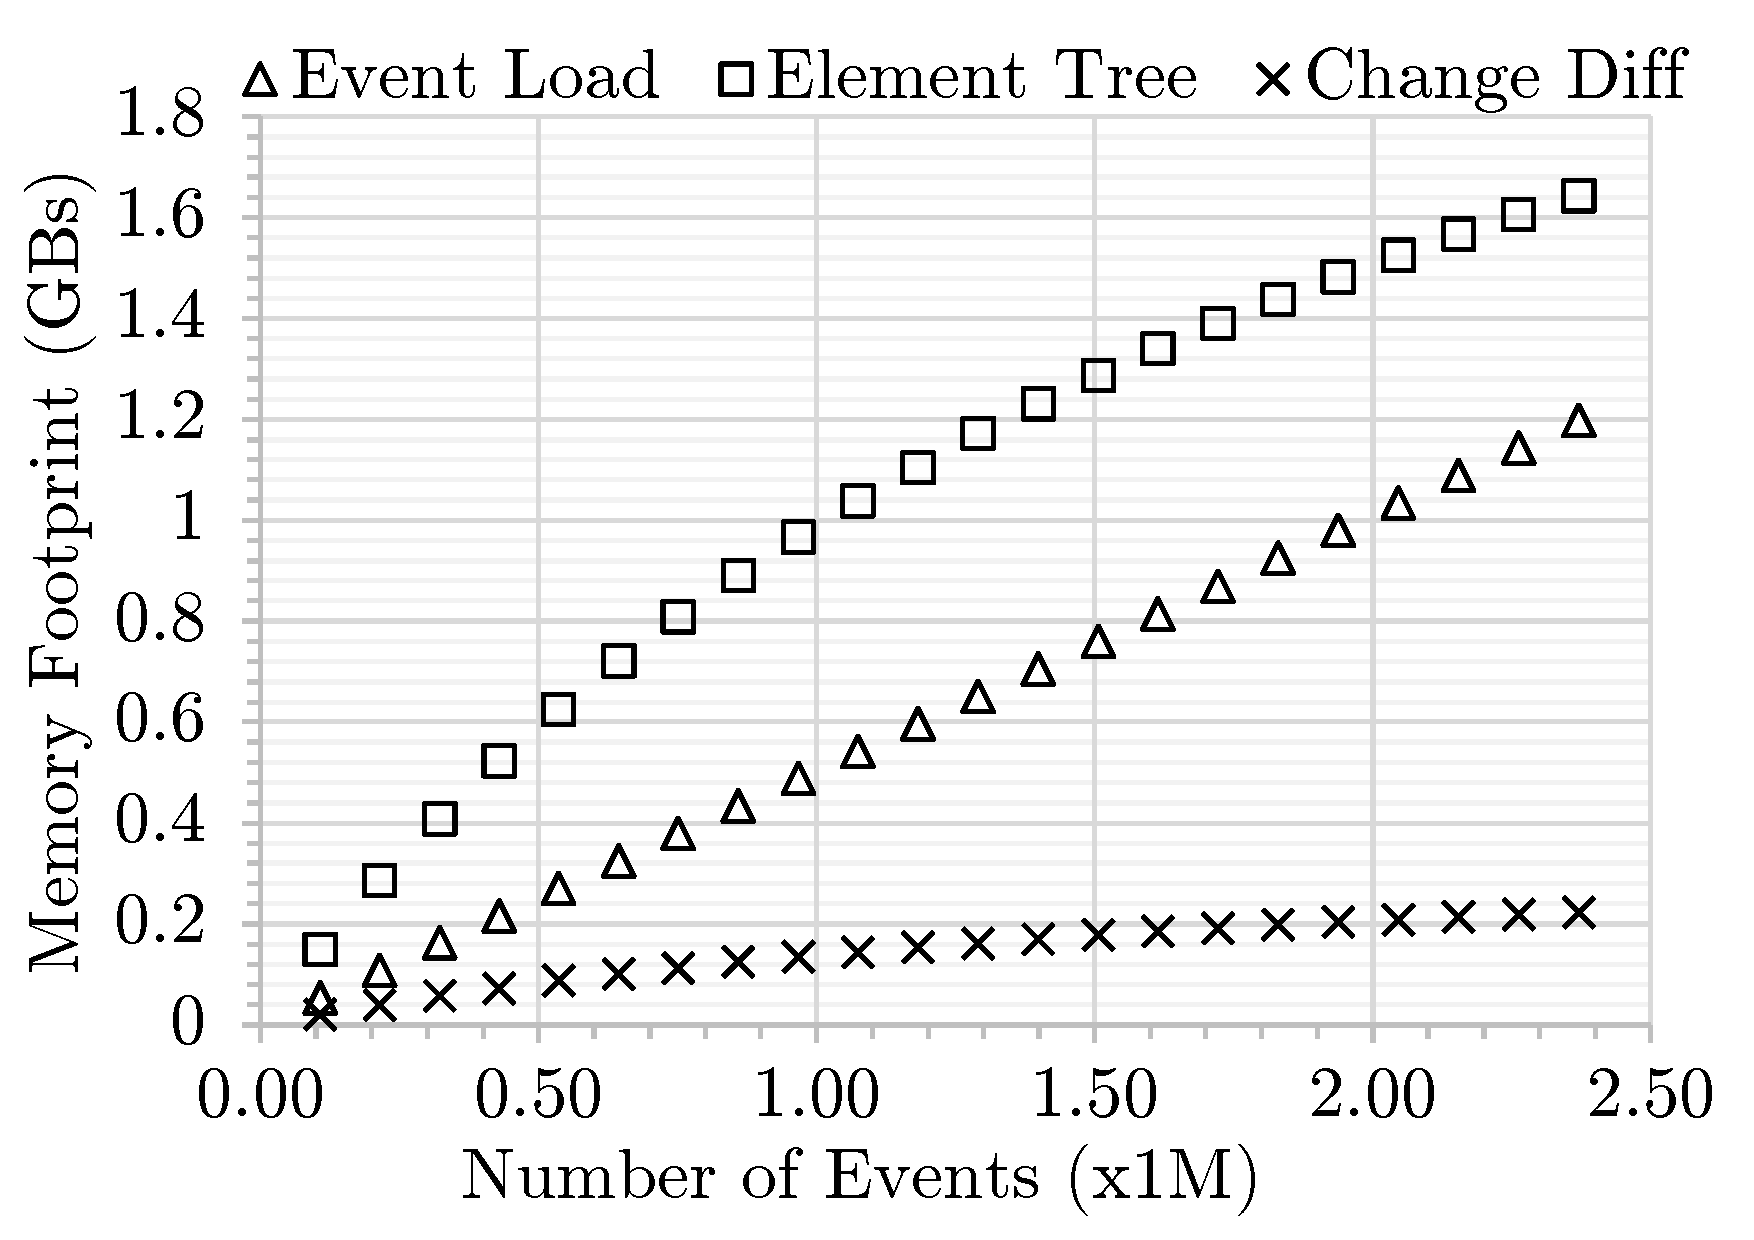
\includegraphics[width=\linewidth]{mixed-memory-events-detail}
        \caption{change-based memory footprint}
        \label{fig:memory_changediff_detail}
    \end{subfigure}
    \hfill
    \begin{subfigure}[t]{0.245\linewidth}
        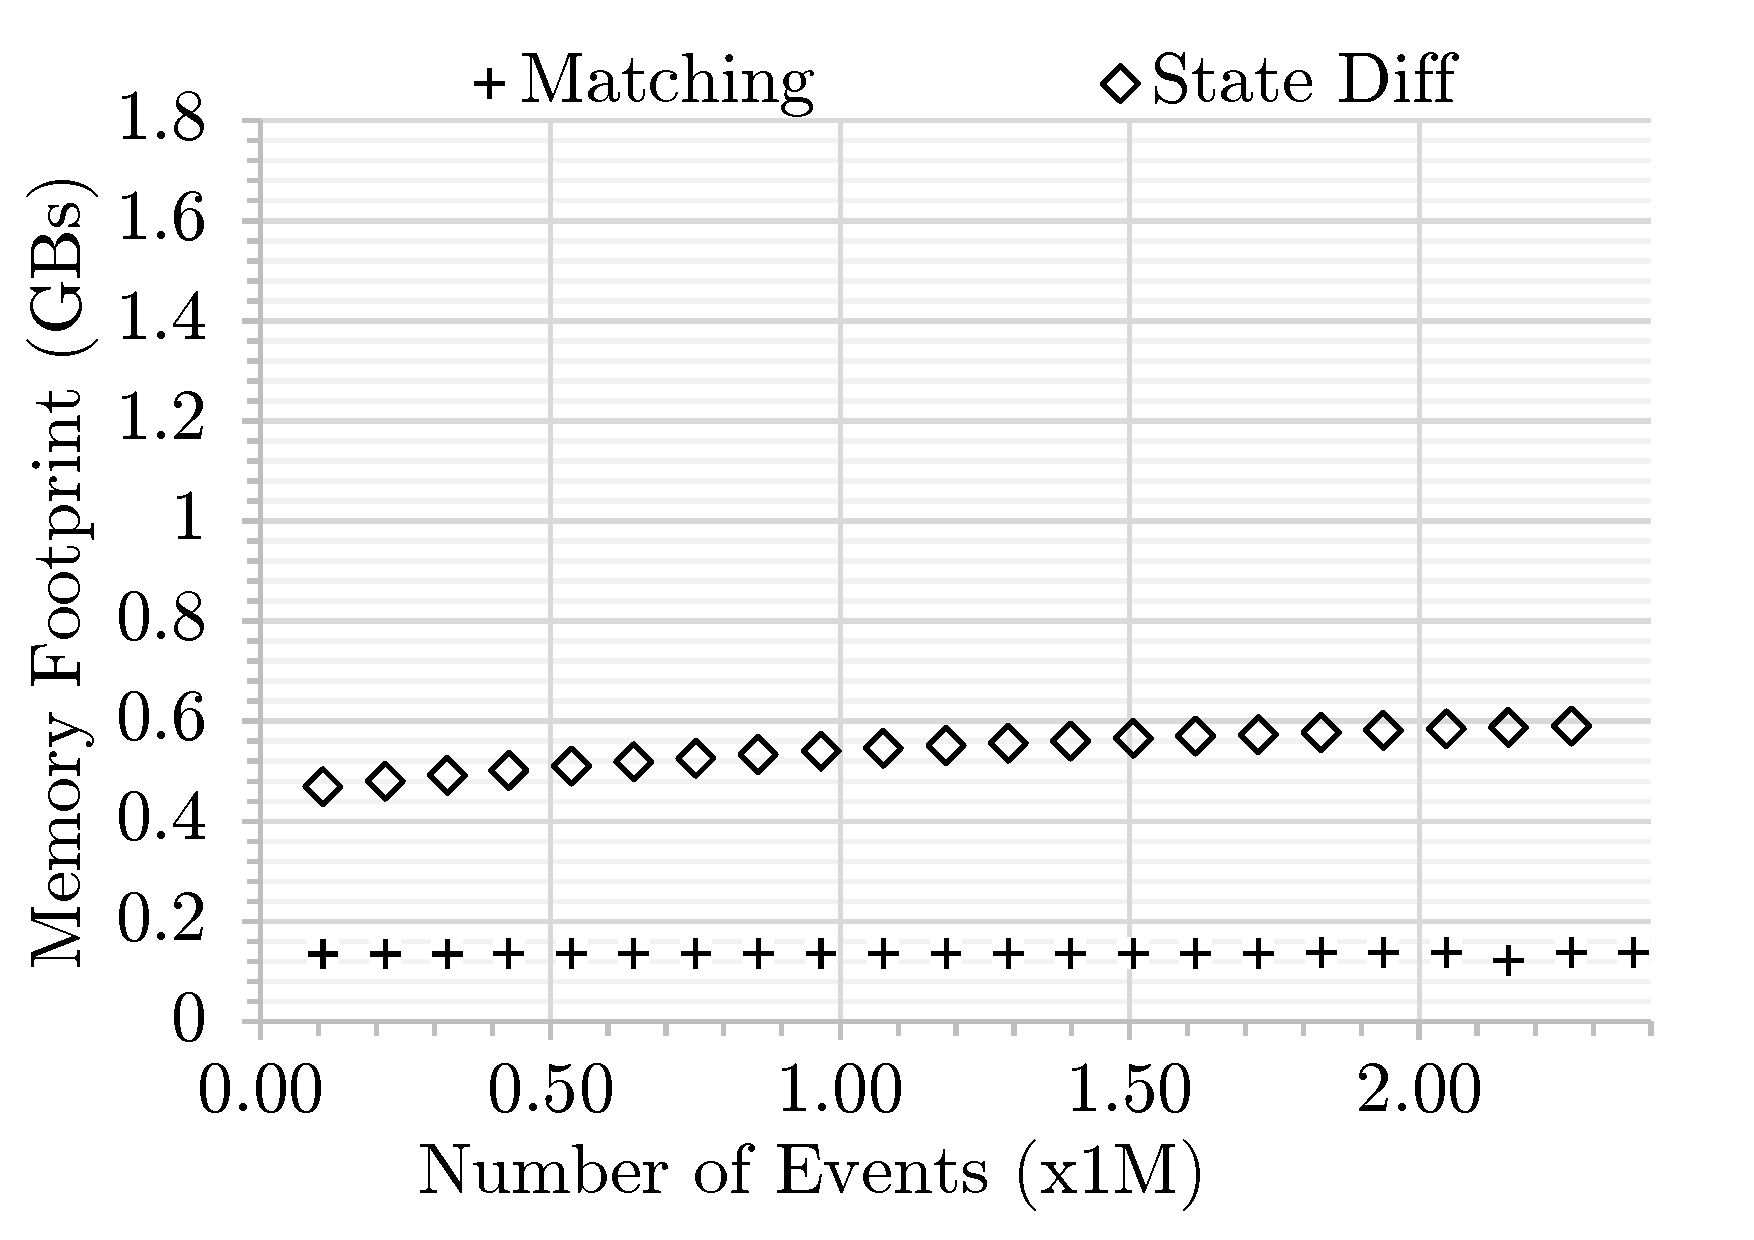
\includegraphics[width=\linewidth]{state-memory-events-detail}
        \caption{state-based memory footprint}
        \label{fig:memory_statediff_detail}
    \end{subfigure}
    \caption{Breakdown view of comparison time and memory footprint in Figure \ref{fig:change_vs_state}.}
    \label{fig:time_memory_detail}
\end{figure*}

For the state-based comparison in Fig. \ref{fig:time_statediff_detail}, the comparison time only experiences a slight increase as the number of identified differences also grows.
%\dk{Change to ``grows''?}. 
This slight increase is contributed mainly by the diffing time, while the matching time tends to be constant due to the very small increase of the total elements (Figures \ref{fig:modification_course}).

Nevertheless, change-based comparison generally consumes more memory than the state-based comparison (see Figure \ref{fig:memory_diffs}). It only consumes less memory than its state-based counterpart when the number of events is less than 0.3 millions (around less than 0.25 million identified differences at that moment). Fig. \ref{fig:memory_changediff_detail} breaks down the memory footprint of change-based comparison into three factors: the loaded change events, element tree, and diffs. As modification continues, an increasing number of events is generated. These events have to be loaded into memory since they contain the required information for the construction of an element tree. The amount of space to keep these change events in memory grows linearly with their number. 

In contrast, the memory used for the element tree grows logarithmically. As the number of events increases, the probability that events modify already affected elements also increases. Thus, no additional memory allocation is required for the element tree. We can also notice that the element tree occupies most of the memory footprint since it mirrors the partial states -- elements, features, and values -- of the models that are affected by the changes. Moreover, in our technical implementation, a feature can have many instances -- one instance for each element (As a comparison, in the EMF implementation, there is only one instance for a feature. The feature is used as a key so that different elements can have the same feature that maps to different values simultaneously). This contributes to the large memory footprint used by the element three. The identified change-based diffs, the third factor, are the smallest factor that contributes to the memory footprint of the change-based comparison. 

For the state-based comparison in Fig. \ref{fig:memory_statediff_detail}, the memory footprint only grows slightly along the increase of differences. A large part of the memory footprint is used to represent the identified differences, while the memory used for matches tends to be constant as the changes of the total elements are very small -- less new elements means less memory needs to be allocated for new matches (Figures \ref{fig:modification_course}). 

\subsubsection{Homogeneous Operations}
\label{sec:homogeneous-operation}

\begin{figure*}[ht]
    \centering
    \begin{subfigure}[t]{0.245\linewidth}
        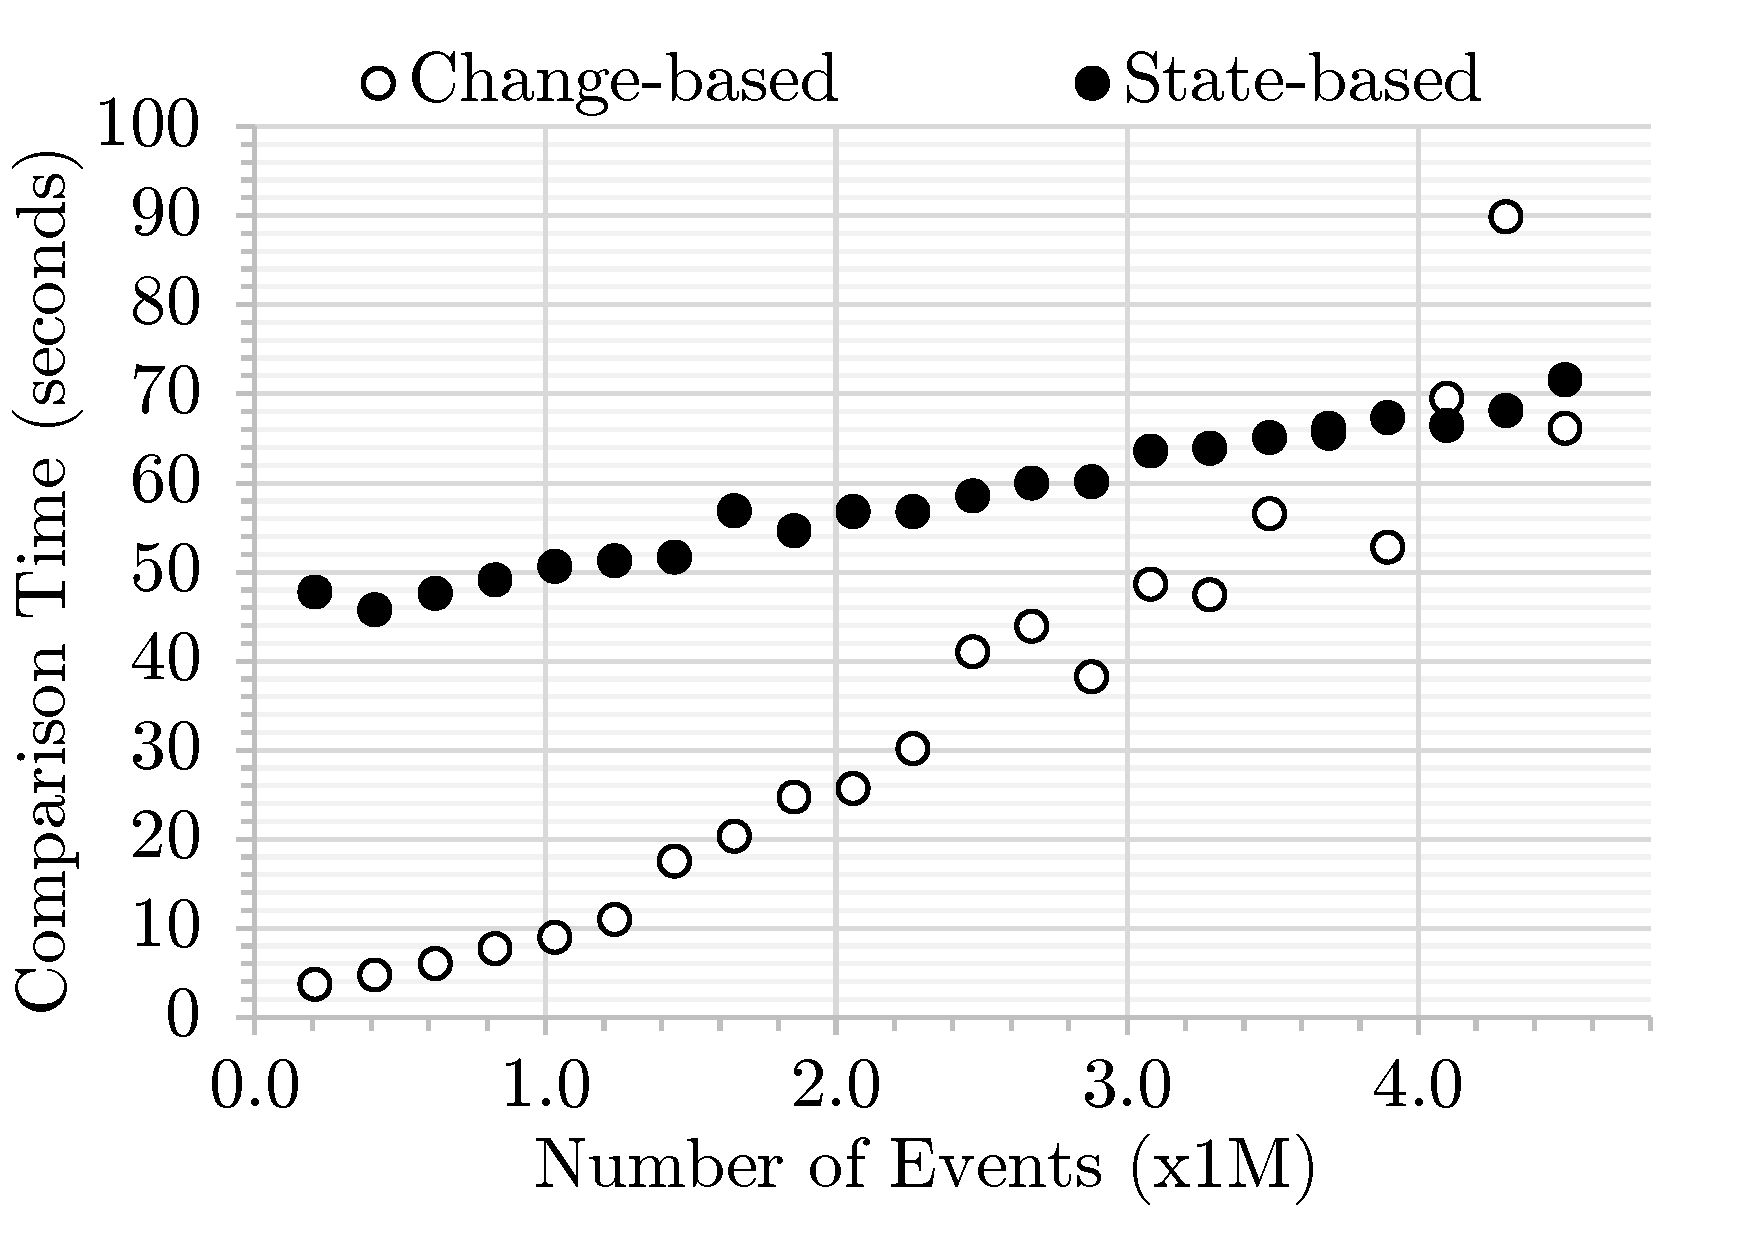
\includegraphics[width=\linewidth]{add-time-events}
        \caption{add-only}
        \label{fig:add-time-events}
    \end{subfigure}
    \hfill
    \begin{subfigure}[t]{0.245\linewidth}
        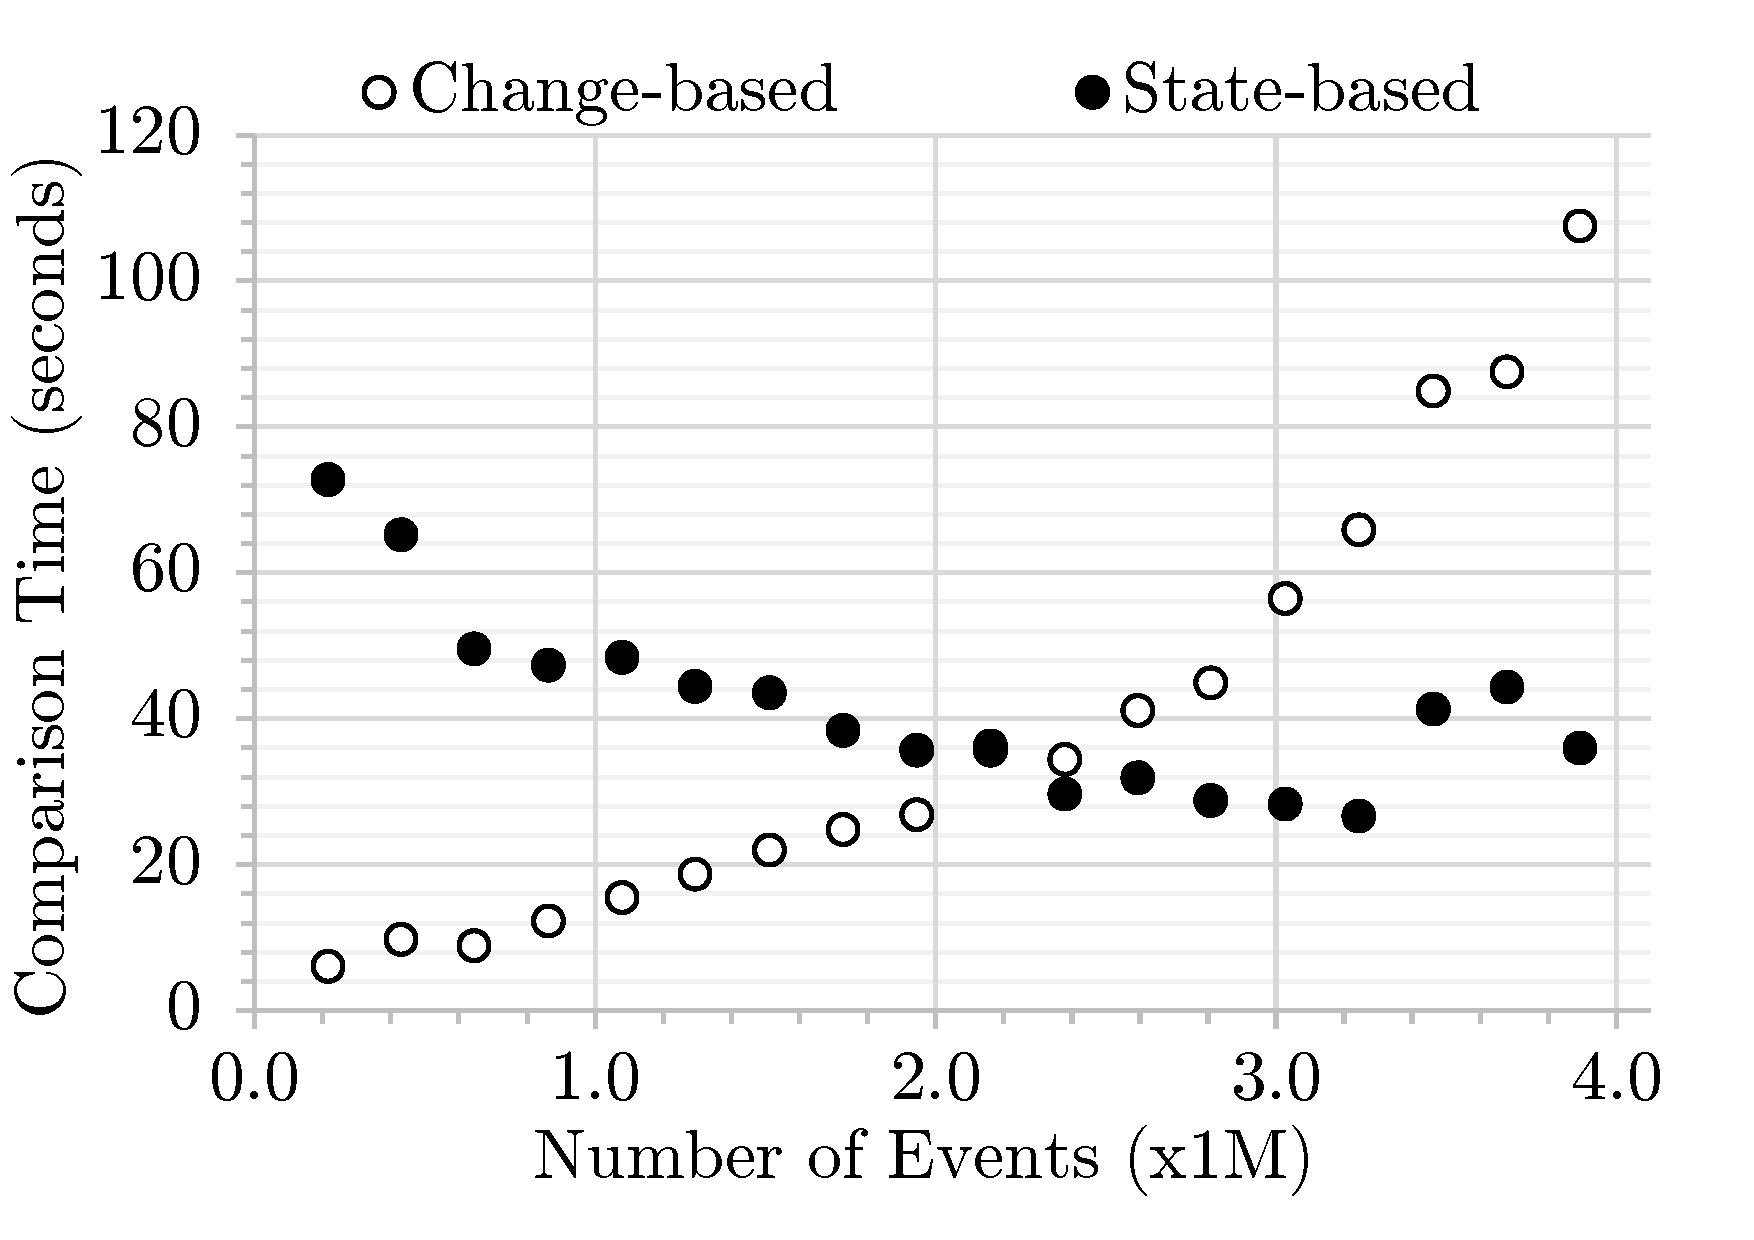
\includegraphics[width=\linewidth]{delete-time-events}
        \caption{delete-only}
        \label{fig:delete-time-events}
    \end{subfigure}
\hfill
    \begin{subfigure}[t]{0.245\linewidth}
        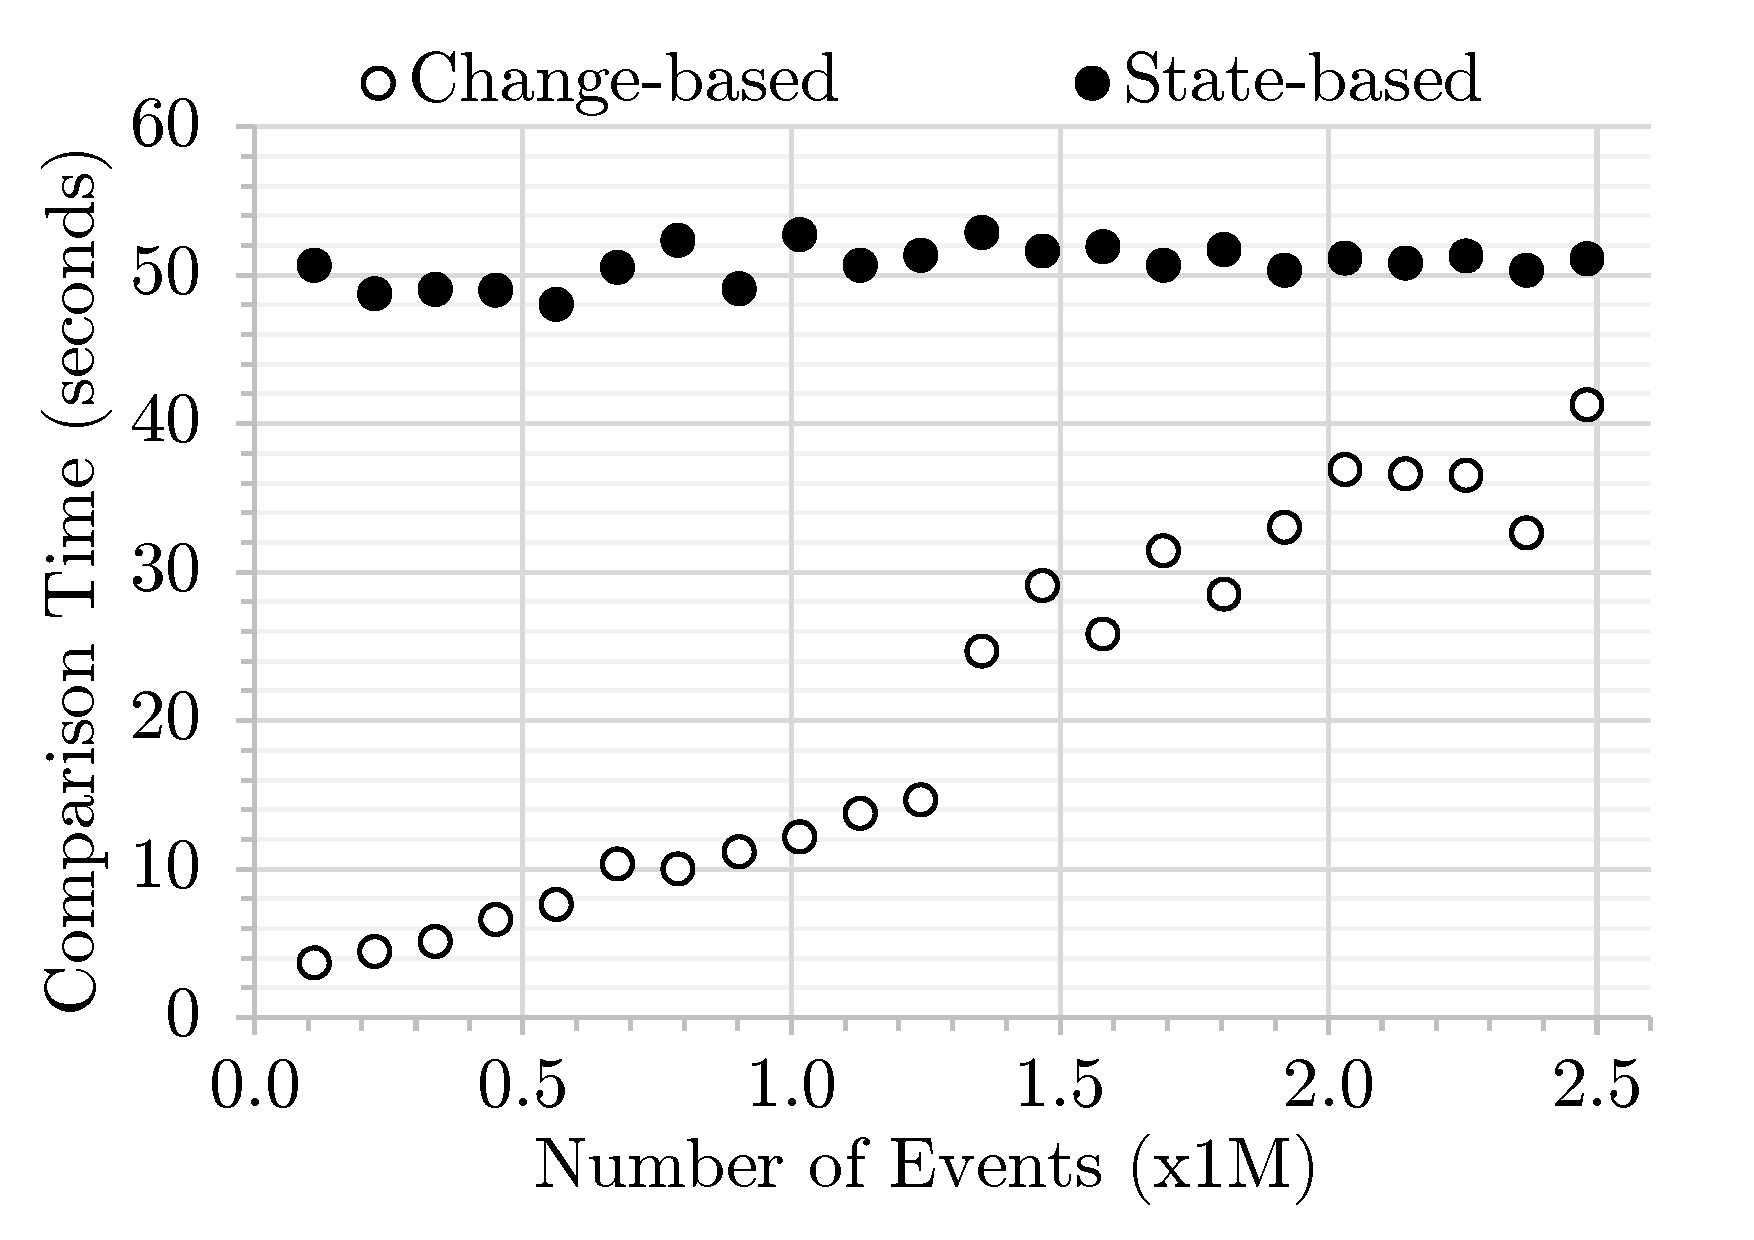
\includegraphics[width=\linewidth]{move-time-events}
        \caption{move-only}
        \label{fig:move-time-events}
    \end{subfigure}
    \hfill
    \begin{subfigure}[t]{0.245\linewidth}
        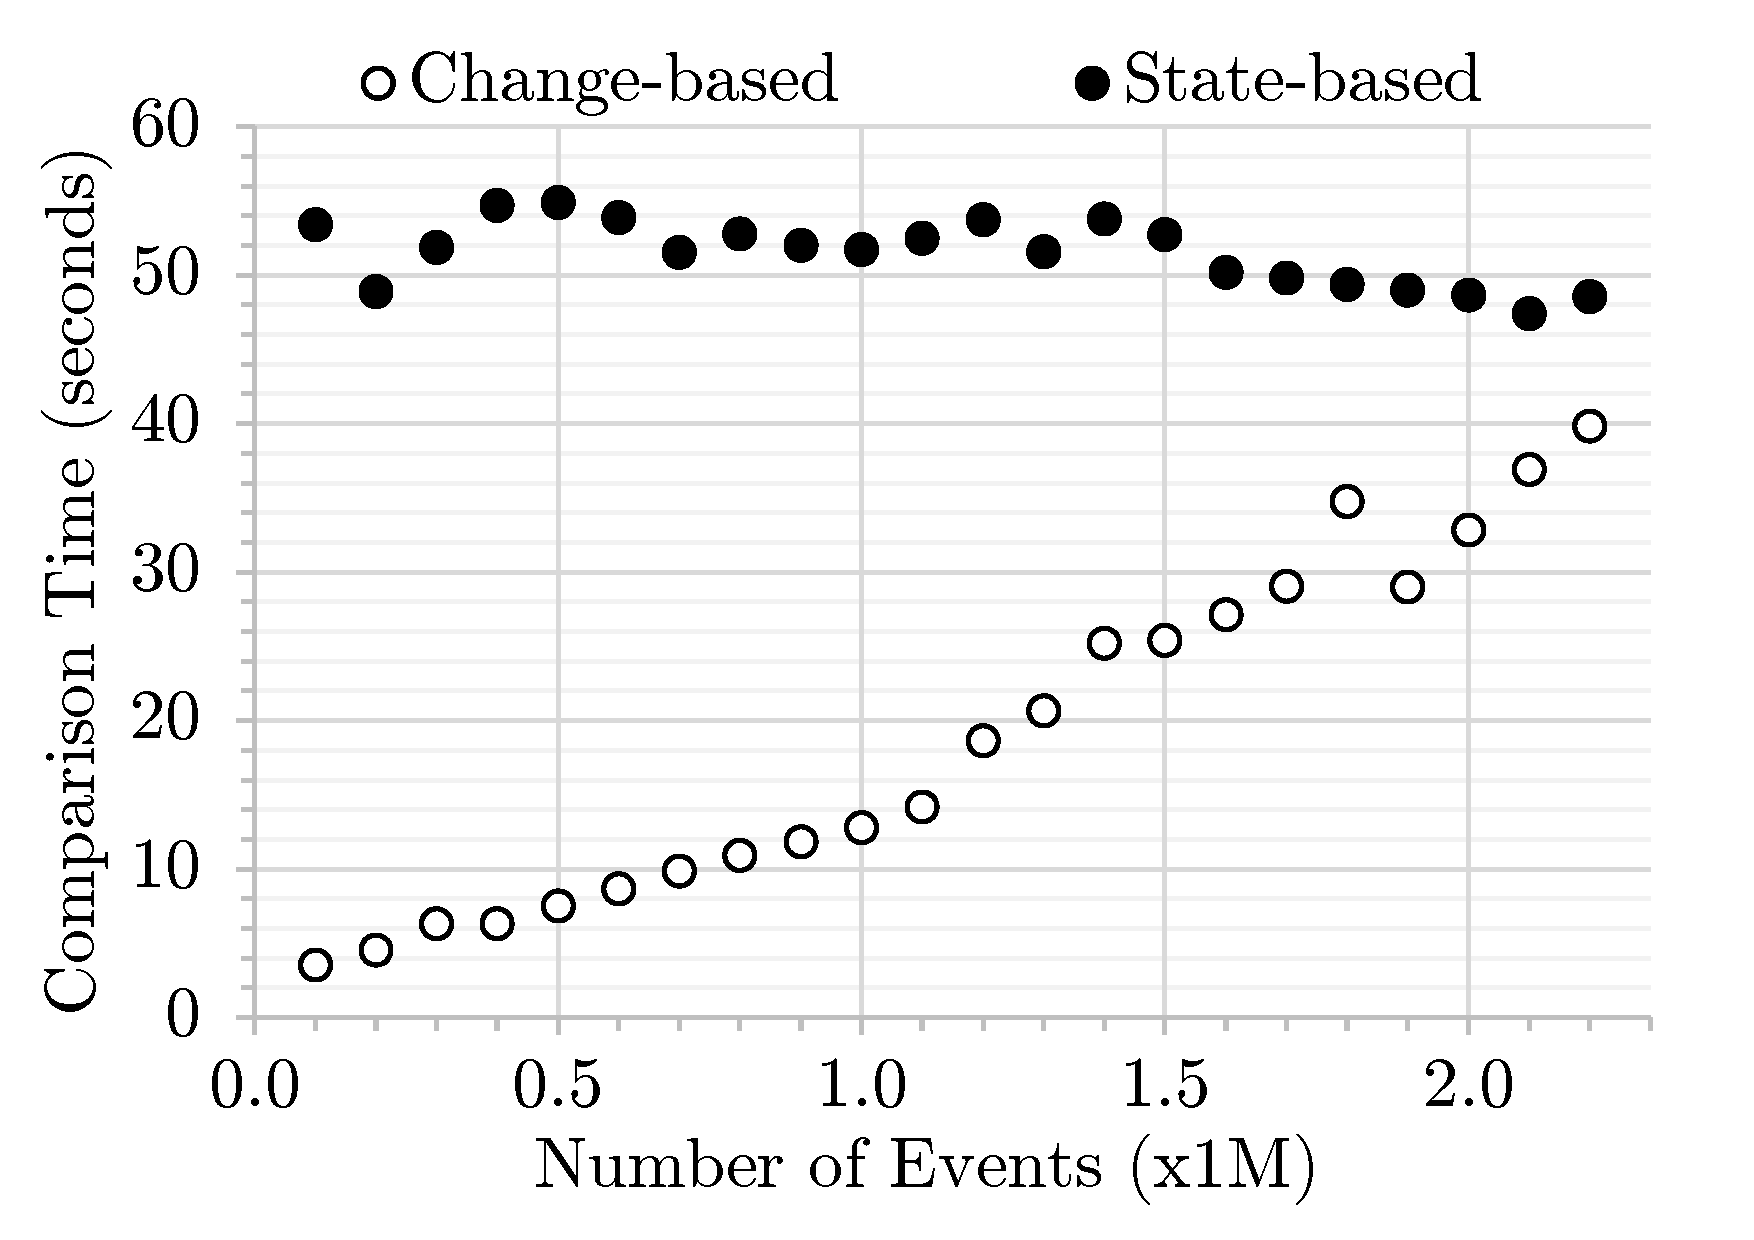
\includegraphics[width=\linewidth]{change-time-events}
        \caption{change-only}
        \label{fig:change-time-events}
    \end{subfigure}
    \caption{Comparison time for homogeneous operations.}
    \label{fig:operation_time_events}
\end{figure*}

\begin{figure*}[ht]
    \centering
    \begin{subfigure}[t]{0.245\linewidth}
        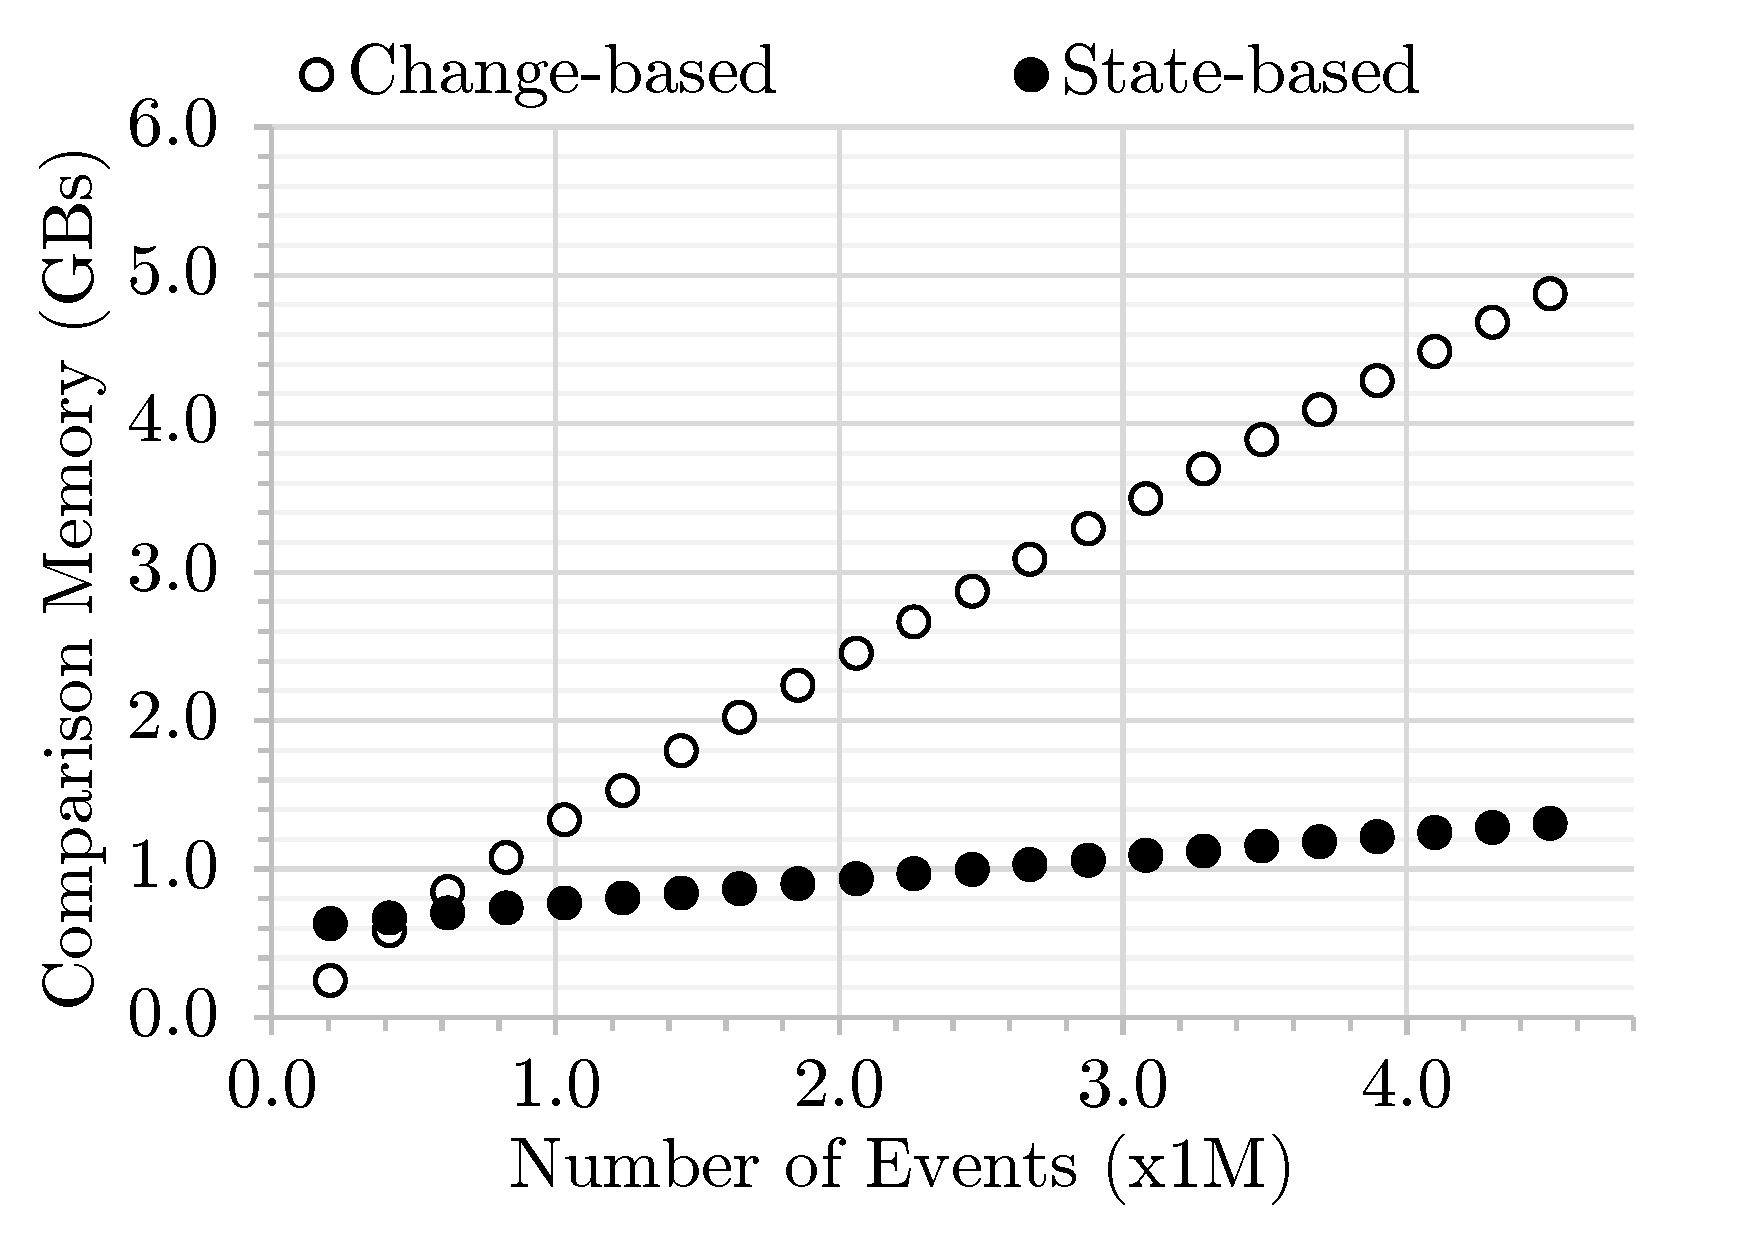
\includegraphics[width=\linewidth]{add-memory-events}
        \caption{add-only}
        \label{fig:add-memory-events}
    \end{subfigure}
    \hfill
    \begin{subfigure}[t]{0.245\linewidth}
        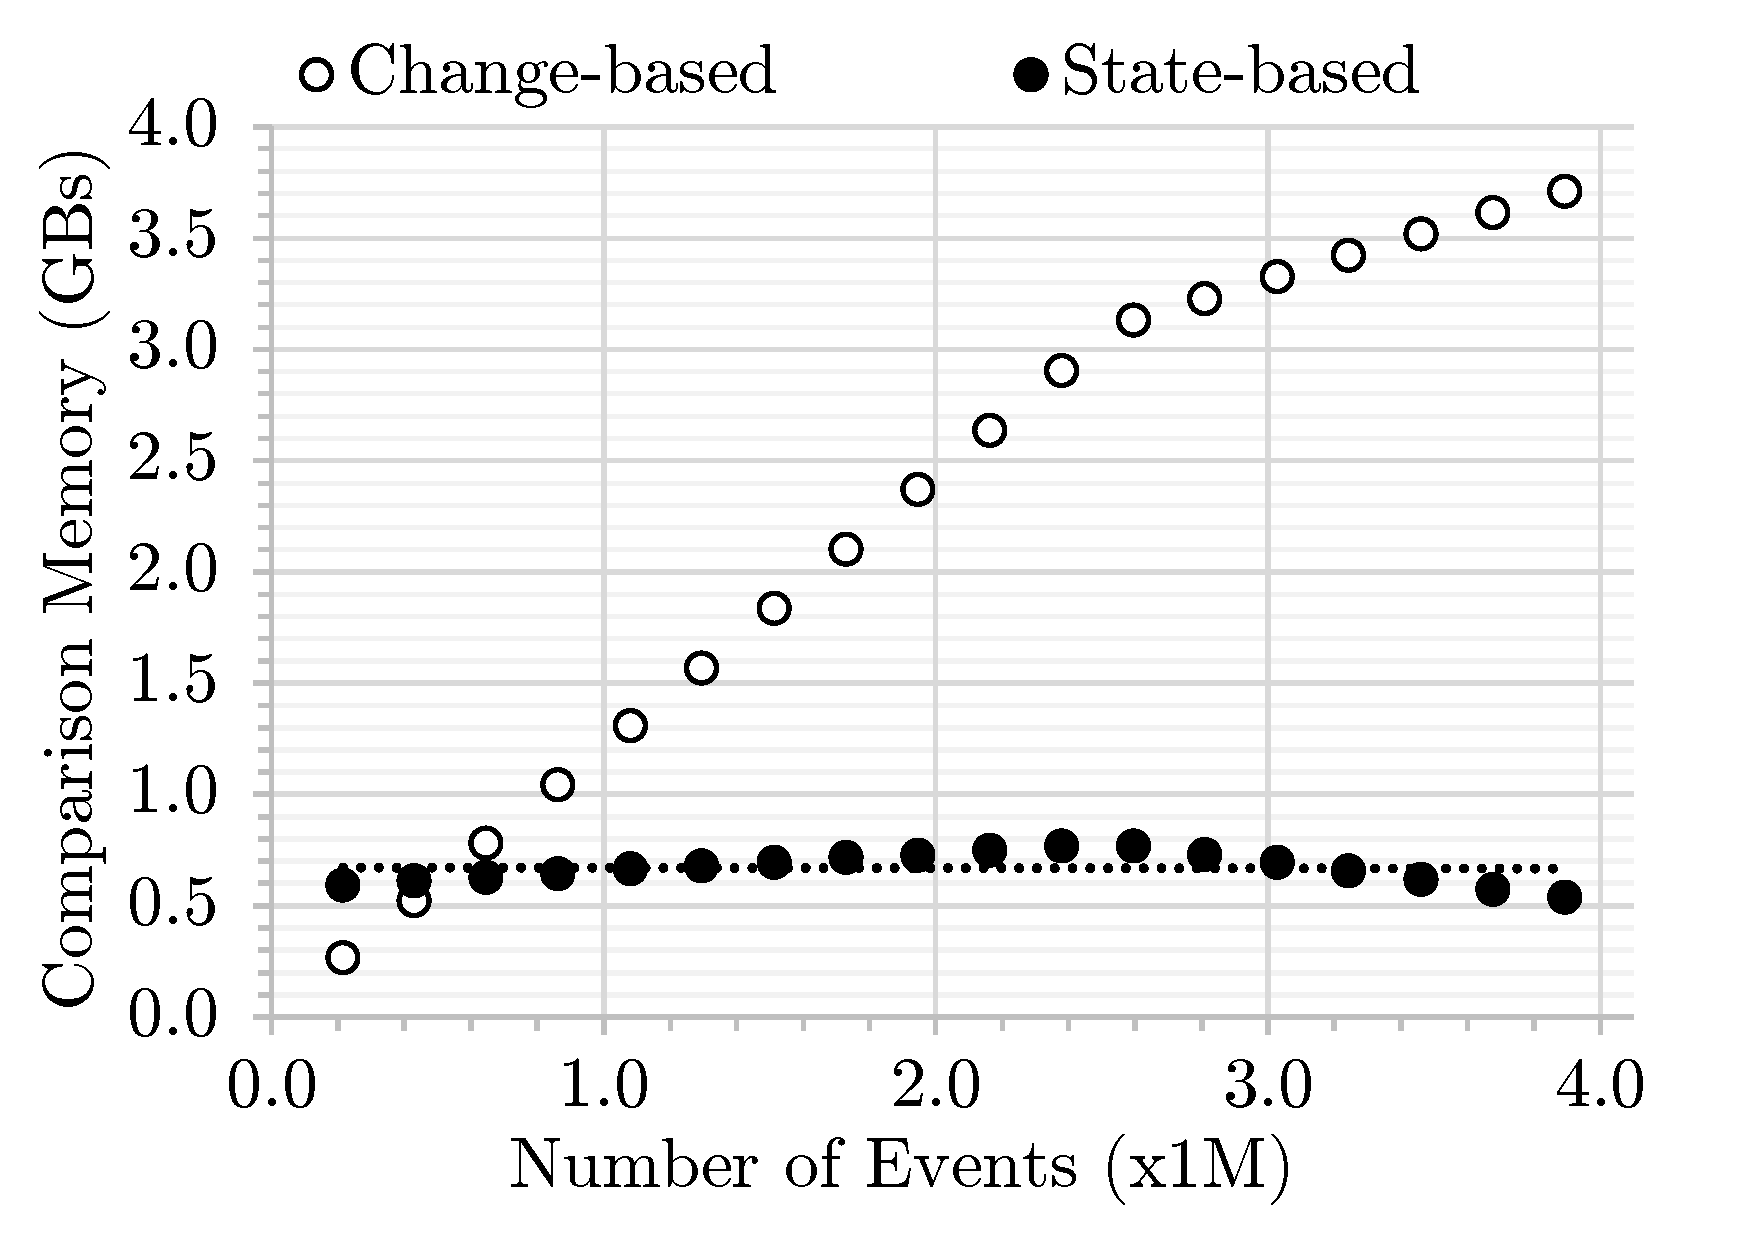
\includegraphics[width=\linewidth]{delete-memory-events}
        \caption{delete-only}
        \label{fig:delete-memory-events}
    \end{subfigure}
\hfill
    \begin{subfigure}[t]{0.245\linewidth}
        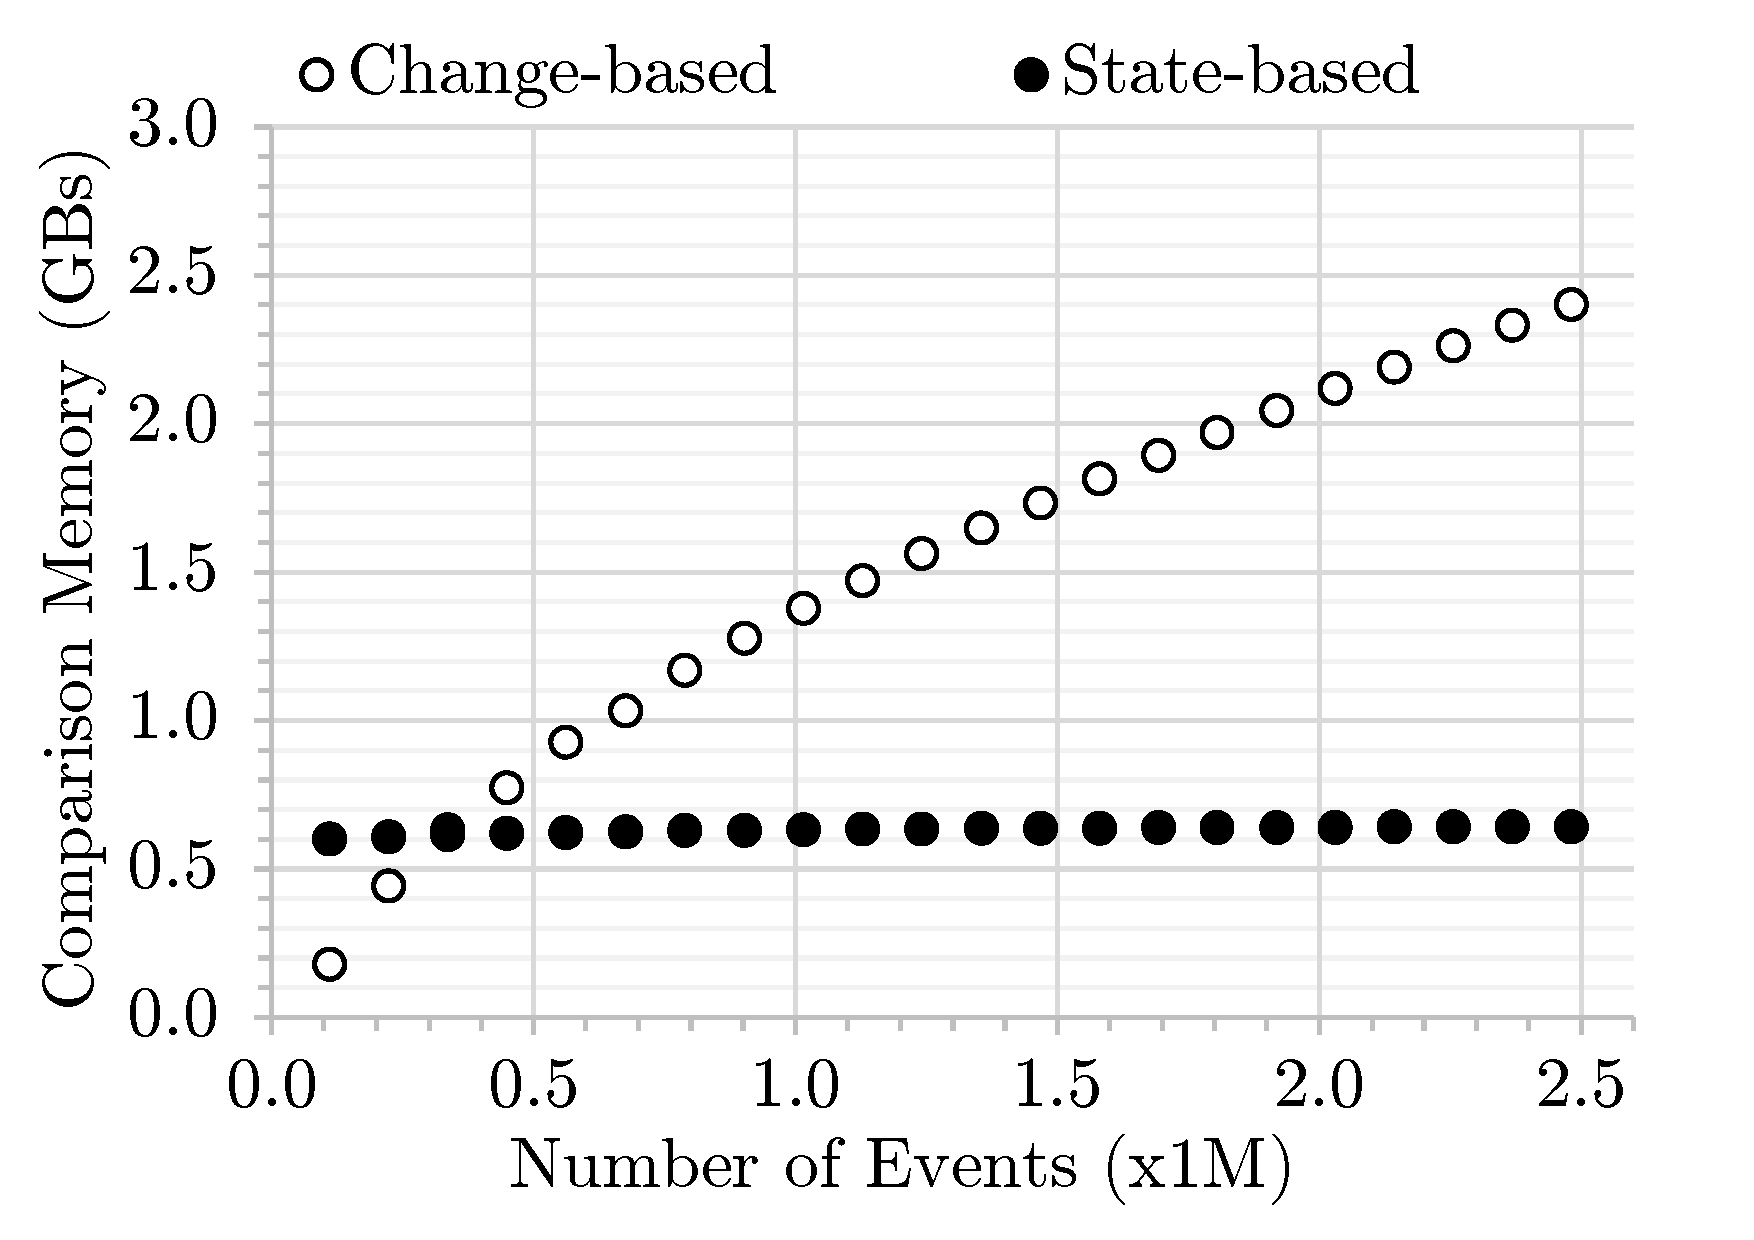
\includegraphics[width=\linewidth]{move-memory-events}
        \caption{move-only}
        \label{fig:move-memory-events}
    \end{subfigure}
    \hfill
    \begin{subfigure}[t]{0.245\linewidth}
        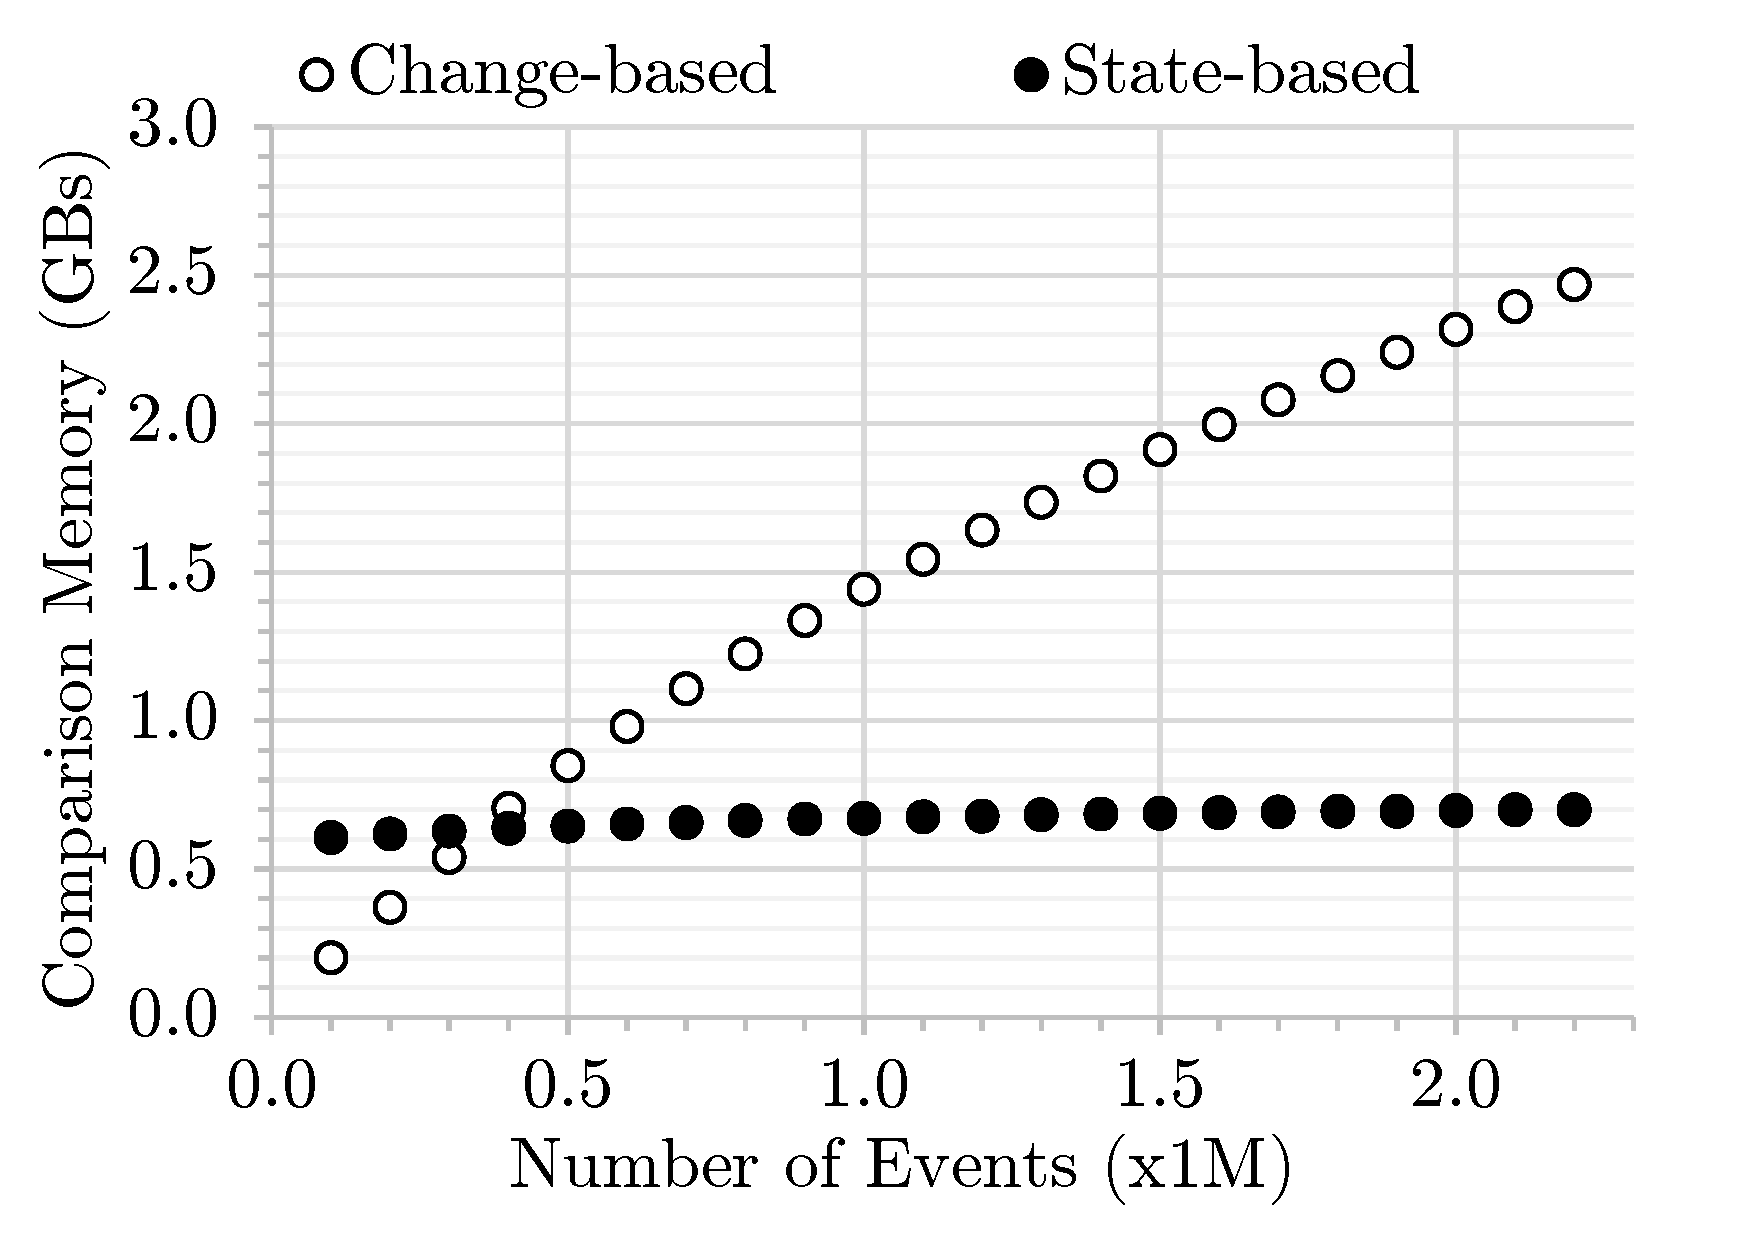
\includegraphics[width=\linewidth]{change-memory-events}
        \caption{change-only}
        \label{fig:change-memory-events}
    \end{subfigure}
    \caption{Memory footprint for homogeneous operations.}
    \label{fig:operation_memory_events}
\end{figure*}

Figures \ref{fig:operation_time_events} and \ref{fig:operation_memory_events} exhibit the comparison time and memory footprint of models that have been modified using homogeneous operations -- \textsf{add}, \textsf{remove}, \textsf{move}, or \textsf{set} only. We can notice that in all figures change-based comparison outperforms its state-based counterpart particularly when the number of change events is small relative to the size of the model. As the number of modifications grows, eventually change-based comparison becomes slower than state-based comparison. In our experiments, this happens when the number of events is greater than 4 million (Fig. \ref{fig:add-time-events}). Change-based comparison also becomes slower when the size of models shrinks (due to a large number of delete events) as depicted in Fig. \ref{fig:delete-memory-events} as the change-based comparison still needs to load these change events and construct its element tree; in contrast, deletion means less work for state-based comparison. In terms of memory footprint, change-based comparison only performs better than state-based comparison when the number of change events is less than 0.3 millions as depicted in Fig. \ref{fig:operation_memory_events}.

\subsection{Conflict Detection}
\label{sec:conflict_results}

\begin{figure*}[ht]
    \centering
    \begin{subfigure}[t]{0.245\linewidth}
        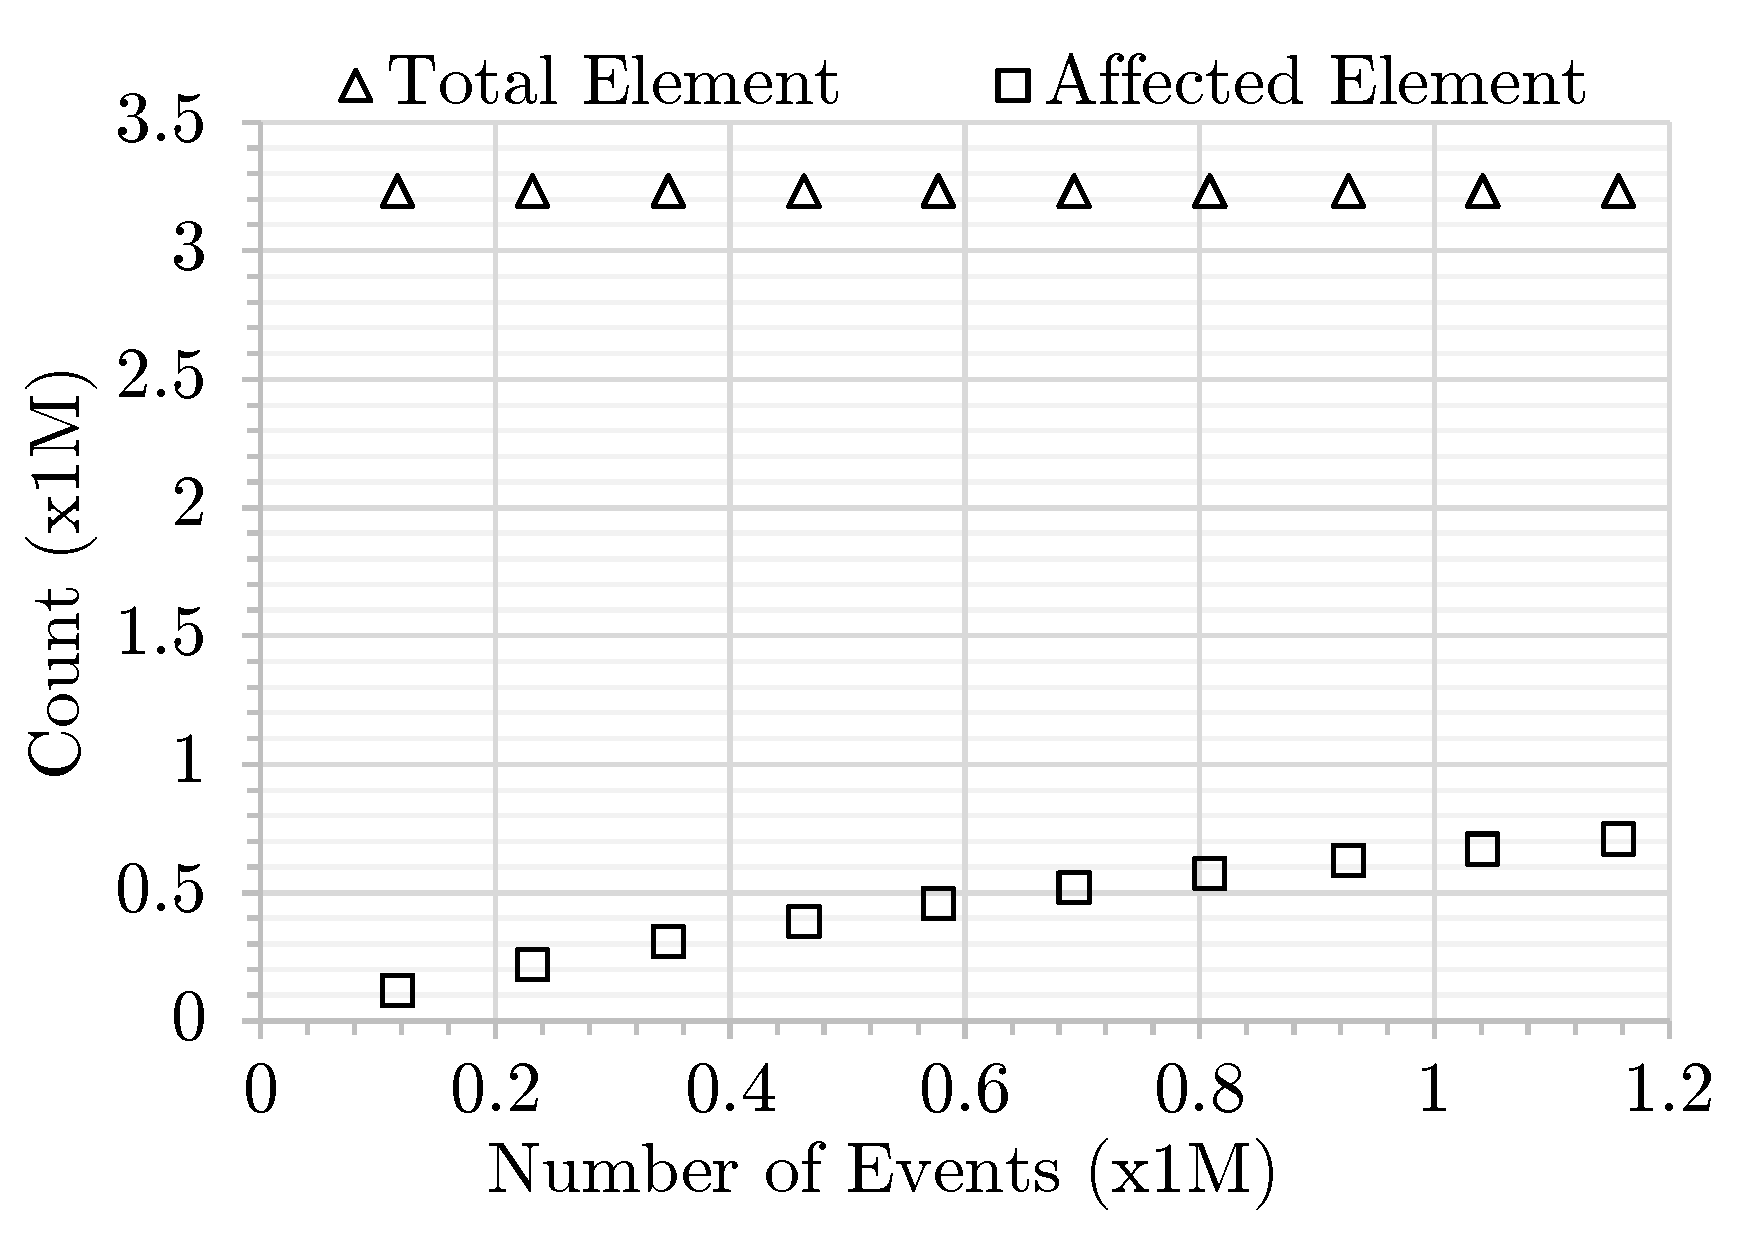
\includegraphics[width=\linewidth]{conflict-size-events}
        \caption{number of elements}
        \label{fig:conflict-size-events}
    \end{subfigure}
    \hfill
    \begin{subfigure}[t]{0.245\linewidth}
        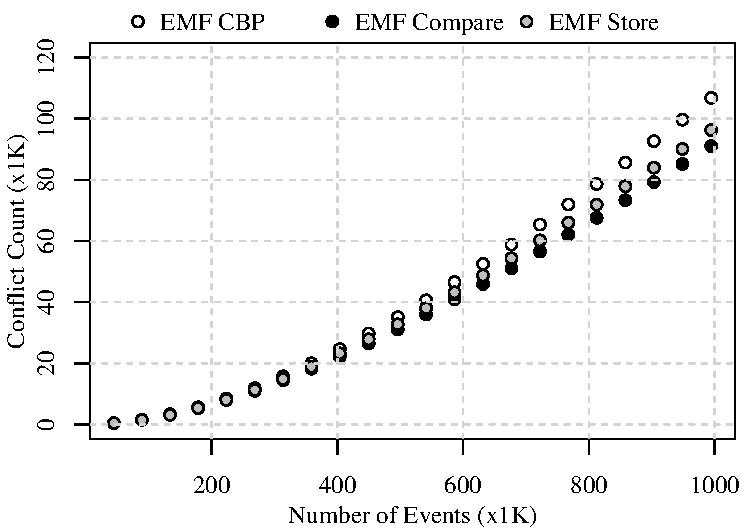
\includegraphics[width=\linewidth]{conflict-count-events}
        \caption{number of conflicts}
        \label{fig:conflict-count-events}
    \end{subfigure}
    \hfill
    \begin{subfigure}[t]{0.245\linewidth}
        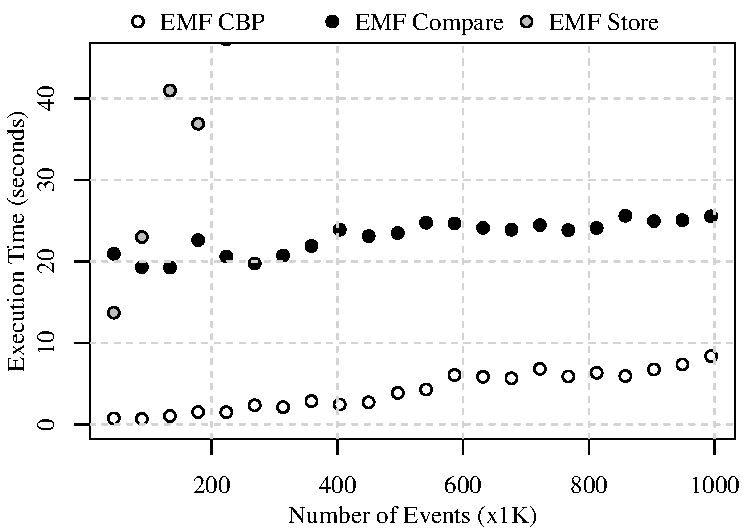
\includegraphics[width=\linewidth]{conflict-time-events}
        \caption{execution time}
        \label{fig:conflict-time-events}
    \end{subfigure}
    \hfill
    \begin{subfigure}[t]{0.245\linewidth}
        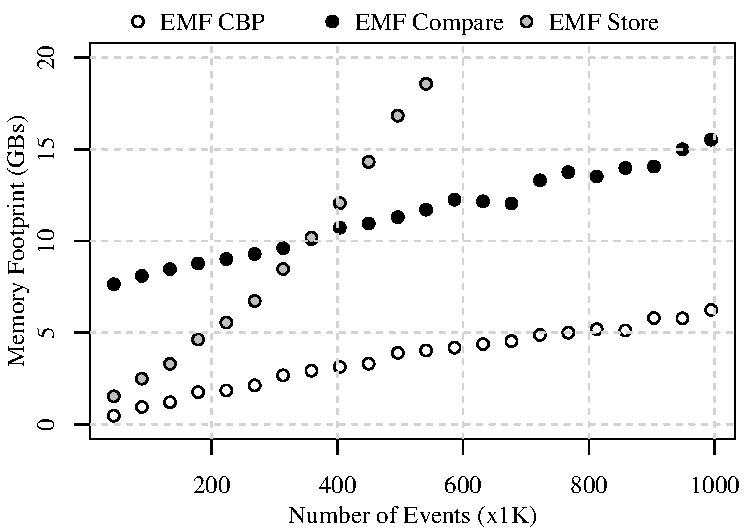
\includegraphics[width=\linewidth]{conflict-memory-events}
        \caption{memory footprint}
        \label{fig:conflict-memory-events}
    \end{subfigure}
    \caption{Epsilon CBP vs. EMF Compare vs. EMF Store comparison as change events increase.}
    \label{fig:conflict_events}
\end{figure*}

This section presents the results of the conflict detection evaluation. Similar to the results in the model differencing evaluation (Fig. \ref{fig:modification_course}), the growing number of change events in the conflict detection evaluation is also followed by the logarithmic increase of affected elements (Fig. \ref{fig:conflict-size-events}). The total number of both elements can also be kept relatively constant due to 1:1 ratio of occurrence of \textsf{add} and \textsf{delete} operations. 

These change events produce different numbers of conflicts for Epsilon CBP, EMF Compare, and EMF Store as can be seen in Fig. \ref{fig:conflict-count-events}. Epsilon CBP detects the least number of conflicts, slightly below the number of conflicts detected by EMF Store. EMF Store detects more conflicts than Epsilon CBP since EMF Store does not consider the eventual states of elements in its conflict detection; it only considers if elements have been changed or not. Moreoever, we can also notice that EMF Compare detects more conflicts than the other two implementations. It is possible since EMF Compare treats constituent conflicts of a composite conflict as separate conflicts. 

Fig. \ref{fig:conflict-time-events} exhibits Epsilon CBP outperforms EMF Compare and EMF Store in terms of execution time in detecting conflicts. In a comparison of two models that consists of around 32 million elements with 1.1 millions change events (the 10th measurement point), Epsilon CBP takes only 4.8 seconds to detect all conflicts while EMF store requires 1 minute and 55 seconds to finish the conflict detection. Both conflict detections are relatively much faster than EMF Compare that needs around 1 hour and 43 minutes to finish detecting conflicts. Fig. \ref{fig:conflict-memory-events} also shows Epsilon CBP outmatches EMF Compare in terms of memory footprint in conflict detection. At the 10th measurement point, Epsilon CBP only consumes around 2.9 GBs which is much lesser than EMF Compare and EMF Store that occupy around 13.9 and 9.8 GBs of memory footprint respectively.

Based on the findings in model differencing and conflict detection evaluation, we argue that the change-based comparison approach works at its best for large models that have been modified a moderate number of times. Models that have been excessively modified and experience significant reduction on model size could impair the performance of change-based comparison as a great number of change records have to be read and loaded into memory. 

\subsection{Limitations and Validity}
\label{sec:limitation_and_Threat_to_validity}
%The proposed change-based comparison comes with a limitation that it heavily relies on the use of identifiers to efficiently address modified elements. Applying change-based persistence to models that use URI fragments as element identifiers faces a challenge in that an element's identifier changes when it is moved to another location in a model.
%\dk{I'm not sure this is a limitation of change-based comparison. Isn't this only relevant when we ``fake'' change-based models?} 
The evaluation of the proposed change-based comparison is limited to the Java metamodel only. Thus, there is no guarantee it will perform in a consistent manner on models conforming to different metamodels. Although, we have tried to cover as much as common changes made in EMF models (e.g. performing \textsf{add}/\textsf{remove}/\textsf{set}/\textsf{move} operations on \textsf{single}/\textsf{multi}-\textsf{valued} features, \textsf{attribute}/\textsf{reference} features, or \textsf{containment}/\textsf{non}-\textsf{containment} references), the random modification made in the evaluation does not largely reflect the evolution of models in the real world. This is challenging as different domains can have their own patterns of model evolution -- different problems, metamodels, modellers, etc.

\section{Related Work}
\label{sec:related_work}
We are not aware of any other work that targets comparison and diffing of change-based models persisted as files. There are however several existing tools for state-based model comparison. Beyond EMFCompare, which we used for our comparative evaluation due to its maturity and ongoing development activity, tools such as SiDiff \cite{Treude2007SiDiff} and DSMDiff \cite{lin2009dsmdiff} also provide language-agnostic graph-based model comparison, with some room for configuration (e.g. assigning different weights to features of types in the language). Additional expressive power -- at the cost of increased complexity and configuration effort -- is offered by dedicated comparison languages such as the Epsilon Comparison Language, which can be used to compare both homogeneous and heterogeneous models \cite{kolovos2009ecl}. We refrain from a more detailed discussion on state-based comparison tools as they all require upfront loading of both versions of the model into memory, which is the main cost that we aspire to reduce with the presented change-based approach.

% SiDiff \cite{Treude2007SiDiff} and DSMDiff \cite{lin2009dsmdiff} treat models as graphs. They create matches and define differences between elements based on the similarity of their features. Both of them offer fixed and language-agnostic comparison and differencing mechanisms However, both are limited in flexibility to exploit the metamodel or particularities of a modelling language \cite{kolovos2009ecl}. EMF Compare \cite{emfcompare2018developer}, an established tool for model comparison and merging, addresses this by providing an extensible platform which users can define custom algorithms for matching, diffing, conflict detection, and merging. Flexibility is also offered by ECL (Epsilon Comparison Language) \cite{kolovos2009ecl}, a hybrid, rule-based language for model comparison, which allows users to specify algorithms to match elements of homogeneous/heterogeneous models.

Database-backed model persistence and version control solutions such as CDO \cite{eclipse2019cdo}, EMFStore \cite{koegel2010emfstore} also provide diffing capabilities between different versions of the same model without requiring models to be fully loaded into memory, however they present integration challenges with mainstream software engineering tools (e.g. continuous integration systems, backup and restore facilities) which are typically file-based, and their performance can degrade as more models/users are added to a repository, since all models are effectively stored in a single database \cite{KolovosRMPGCLRV13}.

% CDO \cite{eclipse2019cdo} is a model repository with pluggable backends. Persisting its models in state-based format limits itself to gain the potential benefits of CBP, such as precise conflict detection and resolution. AMOR \cite{DBLP:conf/sfm/BroschKLSWW12}, a model versioning platform, also compares models in state-based. However, it also uses records of changes/operations of models to improve the precision of conflict detection and resolution. For example, multiple conflicts caused by a composite operation should be resolved as one package, not as an individual conflict, to ensure consistency of resolution. EMFStore \cite{koegel2010emfstore} is a version control system (VCS) for EMF models that stores model versions as packages of operations. Since it works purely in operations without considering the states of models, every operation is treated as a new change. Thus, concurrent operations that change the same feature to the same value are treated as conflicting operations. Solutions that use database backends or dedicated versioning systems (e.g. NeoEMF \cite{daniel2016neoemf}, CDO, EMFStore) demand administrative activities and tight coupling with their backend systems. Our solution prefers text-based file model persistence as it allows users to be benefited by text-based version control systems (e.g. Git, SVN): they are widely-used, robust, and align with the majority of modelling tools that persist models in text-based files.

\vspace{-10pt}
\section{Conclusions and Future Work}
\label{sec:conclusion_and_future_work}
In this paper, we have presented a novel approach to model comparison by exploiting the nature of change-based persistence which allows us to find differences between versions of a model by only comparing the last set of changes between the source and reference model.
Our evaluation results suggest that using this approach, we can produce model comparison that is faster than traditional, state-based model comparison.
However, the change-based comparison approach needs to load change events from a change-based persistence into main memory and thus may requires more memory than for state-based comparison. In our evaluation, this occurs when the number of change events exceeds 400,000.
Arguably, diff and merge operations are usually performed on smaller deltas than our evaluation.
The next challenge for future work is to identify strategies to merge models optimally and persist the merging in the change-based way. 


\subsection{Value Conflict}
This conflict happens when two events change the value of an attribute or non-containment reference into two new different values. 

attribute \& non-containment reference, contaiment vs containment

\subsection{Dependency Conflict}
Delete-other non-create events, Remove-Move

\subsection{Order Conflict}
Ordered: add, remove, move

\subsection{Duplicate Conflict}
NonUnique: add add

%
%\subsection{Subsection title}
%\label{sec:2}
%as required. Don't forget to give each section
%and subsection a unique label (see Sect.~\ref{sec:1}).
%%
%% For one-column wide figures use
%\begin{figure}
%% Use the relevant command for your figure-insertion program
%% to insert the figure file.
%% For example, with the option graphics use
%\resizebox{0.75\textwidth}{!}{%
%  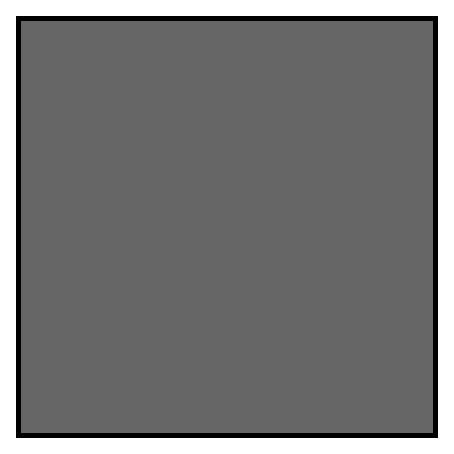
\includegraphics{example.eps}
%}
%% If not, use
%%\vspace{5cm}       % Give the correct figure height in cm
%\caption{Please write your figure caption here}
%\label{fig:1}       % Give a unique label
%\end{figure}
%%
%% For two-column wide figures use
%\begin{figure*}
%% Use the relevant command for your figure-insertion program
%% to insert the figure file. See example above.
%% If not, use
%\vspace*{5cm}       % Give the correct figure height in cm
%\caption{Please write your figure caption here}
%\label{fig:2}       % Give a unique label
%\end{figure*}
%%
%% For tables use
%\begin{table}
%\caption{Please write your table caption here}
%\label{tab:1}       % Give a unique label
%% For LaTeX tables use
%\begin{tabular}{lll}
%\hline\noalign{\smallskip}
%first & second & third  \\
%\noalign{\smallskip}\hline\noalign{\smallskip}
%number & number & number \\
%number & number & number \\
%\noalign{\smallskip}\hline
%\end{tabular}
%% Or use
%\vspace*{5cm}  % with the correct table height
%\end{table}
%%
%% BibTeX users please use
%% \bibliographystyle{}
%% \bibliography{}
%%
%% Non-BibTeX users please use
%\begin{thebibliography}{}
%%
%% and use \bibitem to create references.
%%
%\bibitem{RefJ}
%% Format for Journal Reference
%Author, Journal \textbf{Volume,} (year) page numbers.
%% Format for books
%\bibitem{RefB}
%Author, \textit{Book title} (Publisher, place year) page numbers
%% etc
%\end{thebibliography}

\bibliographystyle{IEEETran}
\bibliography{references}

\end{document}

% end of file template.tex

